
\documentclass{elsarticle}
\bibliographystyle{elsarticle-num}

% ── Package ───────────────────────────────────────────────────────────
\usepackage{amsmath,amssymb,amsfonts,amsthm,bm} % mathamatics
\usepackage{graphicx, float, caption, subcaption} % figures
\usepackage{booktabs,multirow} % tables
\usepackage{hyperref} % hyperlinks
\usepackage{lineno} % line number
\newtheorem{thm}{Theorem}
\newtheorem{rmk}{Remark}
\newtheorem{lma}{Lemma}
\newproof{pf}{Proof}
\linenumbers % turn on line number

% ── Main ──────────────────────────────────────────────────────────────
\begin{document}
%          ╭──────────────────────────────────────────────────────────╮
%          │                       Frontmatter                        │
%          ╰──────────────────────────────────────────────────────────╯
\begin{frontmatter}

% ── Title ─────────────────────────────────────────────────────────────
\title{An optimal volumetric constraint ratio with implementation using mixed FE-Meshfree formulation}
% \title{A Mixed FEM-Meshfree Formulation with Optimal Constraint Ratio for the Divergence--locking Problems}

% ── Author ────────────────────────────────────────────────────────────
\author[1]{Wu Junchao\corref{cor1}}
\ead{jcwu@hqu.edu.cn}
\author[2]{Chu Yingjie}
\author[1]{Xu Yangtao}
\author[2]{Wang Dongdong}

\affiliation[1]{
    organization={
        Key Laboratory for Intelligent Infrastructure and Monitoring of Fujian Province,
        College of Civil Engineering,
        Huaqiao University
    }, 
    city={Xiamen},
    state={Fujian}, 
    postcode={361021},
    country={China},
}

\cortext[cor1]{Corresponding author}

% ── Abstract ──────────────────────────────────────────────────────────
\begin{abstract}
% Formulations for incompressible materials often suffer from volumetric locking, leading to reduced accuracy and oscillatory displacement and pressure solutions.
% A well-chosen constraint ratio can mitigate this issue, but traditional approaches lack a theoretical foundation based on the inf-sup (or LBB) condition, which is essential for the stability of mixed formulations.
% This paper introduces a novel optimal constraint ratio derived from the inf-sup condition to address volumetric locking.
% The inf-sup test, a numerical tool for verifying the inf-sup condition, is reaffirmed as equivalent to inf--sup condition through a variational approach.
% By incorporating a complete polynomial space whose dimension matches the number of displacement degrees of freedom (DOFs),
% a new inf-sup value estimator is developed, explicitly considering the constraint ratio.
% For a given number of displacement DOFs, ensuring that the pressure DOFs remain below a stabilized number falls within the optimal constraint ratio range can satisfy the inf-sup condition.
% To implement of optimal constraint ratio, a mixed finite element and meshfree formulation is proposed,
% where displacements are discretized using traditional finite element approximations, and pressures are approximated via the reproducing kernel meshfree method.
% Leveraging the globally smooth reproducing kernel shape functions,
% the constraint ratio can be flexibly adjusted to meet the inf-sup condition without the limit of element.
% For computational efficiency and ease of implementation, pressure nodes are placed on selected displacement nodes to maintain the optimal constraint ratio.
% Inf-sup tests and a series of 2D and 3D elasticity examples validate the proposed constraint ratio, demonstrating its effectiveness in eliminating volumetric locking and enhancing the performance of mixed finite element and meshfree formulations.

Formulations for incompressible materials often suffer from volumetric locking, leading to reduced accuracy and oscillatory displacement and pressure solutions.
A well-chosen constraint ratio can mitigate this issue, but traditional approaches lack a theoretical foundation based on the inf-sup (or LBB) condition, which is essential for the stability of mixed formulations.
This paper introduces a novel optimal constraint ratio derived from the inf-sup condition to address volumetric locking.
The inf-sup test, a numerical tool for verifying the inf-sup condition, is reaffirmed as equivalent to the inf-sup condition through a variational approach.
By incorporating a complete polynomial space whose dimension matches the number of displacement degrees of freedom (DOFs), a new inf-sup value estimator is developed, explicitly considering the constraint ratio.
For a given number of displacement DOFs, ensuring that the pressure DOFs remain below a stabilized number falls within the optimal constraint ratio range can satisfy the inf-sup condition.
To implement the optimal constraint ratio, a mixed finite element and meshfree formulation is proposed, where displacements are discretized using traditional finite element approximations, and pressures are approximated via the reproducing kernel meshfree method.
Leveraging the globally smooth reproducing kernel shape functions, the constraint ratio can be flexibly adjusted to meet the inf-sup condition without the limit of element.
For computational efficiency and ease of implementation, pressure nodes are placed on selected displacement nodes to maintain the optimal constraint ratio.
Inf-sup tests and a series of 2D and 3D elasticity examples validate the proposed constraint ratio, demonstrating its effectiveness in eliminating volumetric locking and enhancing the performance of mixed finite element and meshfree formulations.
\end{abstract}

% ── Keywords ──────────────────────────────────────────────────────────
\begin{keyword}
    Optimal constraint ratio
    \sep
    Inf--sup condition estimator
    \sep
    Volumetric locking
    \sep
    Mixd formulation
    \sep
    Reproducing kernel meshfree approximation
\end{keyword}

\end{frontmatter}


\section{Introduction}

% The volumetric constraint is a necessary condition in the formulation of incompressible materials
% like rubber and hydrogel.
% Proper imposition of this constraint is crucial for obtaining better numerical solutions;
% insufficient or excessive constraints will reduce the accuracy and stability of the solution \cite{brezzi1991a}.
% The volumetric constraint ratio \cite{hughes2000}, denoted as $r$, is often used to measure the level of constraint. 
% It is defined as the total degrees of freedom (DOFs) of displacement divided by the total DOFs of pressure.
% Ideally, the optimal constraint ratio should be consistent with its governing partial differential equations.
% For example, in the two-dimensional (2D) case, the optimal constraint ratio is 2, since there are two governing equations for displacement and one for pressure.
% When the constraint ratio is less than 2, the formulation suffers from volumetric locking, while a constraint ratio greater than 2 can cause a coarse solution for pressure.
% These observations have been summarized by pioneering work \cite{hughes2000} as follows:
% \begin{equation}
% r = \frac{2n_u}{n_p}, \quad 
% \begin{cases}
% r > 2 & \text{too few constraints} \\
% r = 2 & \text{optimal} \\
% r < 2 & \text{too many constraints} \\
% r \le 1 & \text{severe locking} \\
% \end{cases}
% \end{equation}
% where $n_u$ and $n_p$ are the number of control nodes for displacement and pressure, respectively.
% Classifying the locked status via the constraint ratio is straightforward but imprecise.
% For instance, the constraint ratio can remain 2 while the pressure is discretized using continuous shape functions identical to the displacement's approximation.
% However, volumetric locking still exists in this formulation \cite{hughes2000}.

% The inf--sup condition, also known as the Ladyzhenskay--Babuška--Brezzi (LBB) condition \cite{babuska1997a,bathe1996}, is a more precise requirement for a locking--free formulation.
% This condition is based on the mixed formulation framework, and when the inf--sup condition is satisfied, both the accuracy and stability of the mixed-formulation can be ensured.
% However, verifying the inf--sup condition is non-trivial.
% An eigenvalue problem namely inf--sup test can be used to check this condition numerically \cite{malkus1981,chapelle1993,brezzi,gallistl2019}.
% Analytically, Brezzi and Fortin proposed a two-level projection framework that always satisfies the inf-sup condition,
% allowing it to be checked by identifying whether the formulation is included in this framework.
% Both analytical and numerical methods to check the inf-sup condition are complex,
% and the relationship between the constraint ratio and the inf-sup condition remains unclear.

% To address volumetric constraint issues, adjusting the constraint ratio to an appropriate level is commonly used and easily implemented.
% In traditional finite element methods (FEM), this adjustment is carried out based on elements since the DOFs are embedded in each element.
% Conventional FEM often exhibits an over--constrained status.
% Reducing the approximation order of pressure in mixed formulation can alleviate the constraint burden, such as with the well-known Q4P1 (4--node quadrilateral displacement element with 1--node piecewise constant pressure element) and Q8P3.
% Globally, using continuous shape functions to link the local pressure DOFs in each element can also reduce the total number of pressure DOFs and increase the constraint ratio, such as with T6P3 (6--node triangular displacement element with 3--node continuous linear pressure element) and Q9P4 (Taylor--Hood element) \cite{hood1974}.
% These schemes belong to the mixed formulation framework and can also be implemented through a projection approach, where the pressure approximant is projected into a lower--dimensional space.
% Examples include selective integration methods \cite{malkus1978,shilt2020}, B--bar or F--bar methods \cite{simo1990,broccardo2009,coombs2018,saloustros2021,rodriguez2023}, pressure projection methods \cite{simo1985,dohrmann2004}, and the enhanced strain method \cite{lovadina2003}.
% Meanwhile, conventional 3--node triangular elements arranged in a regular cross pattern can also reduce the dimension of the pressure space \cite{bathe2001}.
% It should be noted that not all of these methods can meet the inf--sup condition despite alleviating volumetric locking and producing a good displacement solution.
% Some methods, like Q4P1, show significant oscillation for the pressure solution, known as spurious pressure mode or checkerboard mode \cite{bathe2001}.
% In such cases, additional stabilization approaches, such as multi-scale stabilization (VMS) \cite{hughes1995,masud2005,rossi2021,karabelas2022} or Galerkin/least-squares (GLS) \cite{hughes1986}, are required to eliminate the oscillations in pressure.

% Another class of FEM methods adjusts the constraint ratio by increasing the displacement DOFs.
% For instance, based on 3--node triangular elements, Arnold et al. used a cubic bubble function in each element to increase the displacement DOFs, known as the MINI element \cite{arnold1984,auricchio2005}.
% It has been shown that this method belongs to the VMS framework \cite{quarteroni1994}, and its fulfillment of the inf--sup condition can be analytically evidenced using the two--level projection framework \cite{brezzi}.
% The Crouzeix--Raviart element \cite{crouzeix1973} transfers the DOFs from the triangular vertices to edges, increasing the constraint ratio since, for triangular topology, the number of edges is greater than that of vertices.
% More details about FEM technology for divergence constraint issues can be found in Refs. \cite{hughes2000,bathe1996,brink1996}.

% In the past two decades, various novel approximations equipped with global smoothed shape functions, such as moving least-squares approximation \cite{belytschko1994}, reproducing kernel approximation \cite{liu1995}, radial basis functions \cite{chi2014,wang2020d}, maximum-entropy approximation \cite{ortiz-bernardin2015}, and NURBS approximation \cite{hughes2005,auricchio2010}, have been proposed.
% In these approaches, the approximant pressure evaluated by the derivatives of global continuous shape functions also maintains a constraint ratio of 2 in 2D incompressible elasticity problems.
% However, the corresponding results still show lower accuracy caused by locking \cite{huerta2001,dolbow1999a}.
% Widely--used locking--free technologies for FEM are introduced in these approaches to enhance their performance.
% For example, Moutsanidis et al. employed selective integration and B--bar, F--bar methods for reproducing kernel particle methods \cite{moutsanidis2020,moutsanidis2021}.
% Wang et al. applied selective integration schemes with bubble--stabilized functions to node--based smoothed particle FEM \cite{wang2022c}.
% Elguedj et al. proposed the B--bar and F--bar NURBS formulations for linear and nonlinear incompressible elasticity.
% Chen et al. adopted the pressure projection approach for reproducing kernel formulations for nearly--incompressible problems \cite{chen2000}, which was later extended to Stokes flow formulations by Goh et al. \cite{goh2018}.
% Bombarde et al. developed a block--wise NURBS formulation for shell structures, eliminating locking via pressure projection \cite{bombarde2022}.
% Most of these approximations offer better flexibility for arranging DOFs since their shape function constructions are no longer element-dependent.
% Huerta et al. proposed a reproducing kernel approximation with divergence-free basis functions to avoid volumetric strain entirely \cite{huerta2004a}, although this approach is unsuitable for compressible cases.
% Wu et al. added extra displacement DOFs in FEM elements to resolve the locking issue, constructing local shape functions using generalized meshfree interpolation to maintain consistency \cite{wu2012}.
% Vu--Huu et al. employed different--order polygonal finite element shape functions to approximate displacement and pressure, embedding a bubble function in each element for stabilization.

% This work proposes a more precise optimal divergence constraint ratio and implements a locking--free mixed FEM--Meshfree formulation with this optimal constraint ratio.
% Firstly, the inf--sup condition is derived in a new form, showing that the inf--sup value equals the lowest non--zero eigenvalue of dilatation stiffness in the context of variational analysis.
% Subsequently, involving a complete polynomial space with dimensions identical to displacement DOFs, the number of non--zero eigenvalues can be analytically calculated,
% and a new estimator considering the constraint ratio is established.
% From this estimator, the optimal constraint ratio is defined with a stabilized number of pressure nodes.
% If the constraint ratio exceeds the locking ratio, the formulation will show severe locking.
% When the constraint ratio is lower than the optimal ratio, the formulation achieves satisfactory results, and the inf--sup condition is fulfilled.
% This estimator provides a strong link between the inf--sup value and the pressure DOFs, making it possible to justify the locking status by counting the pressure nodes.
% Furthermore, a mixed FEM-Meshfree formulation is proposed to verify the optimal constraint ratio.
% In this mixed formulation, the displacement is approximated by traditional finite element methods, and the pressure is discretized by reproducing kernel meshfree approximation.
% With the aid of global RK shape functions, the pressure's DOFs can be adjusted arbitrarily without considering approximation order and numerical integration issues to maintaining the constraint ratio as optimal.

% The remainder of this paper is organized as follows:
% Section 2 reviews the mixed-formulation framework for incompressible elasticity problems.
% In Section 3, a novel estimator of the inf-sup value is developed, from which the optimal constraint ratio is obtained.
% Section 4 introduces the mixed FEM-Meshfree formulation and its corresponding nodal distribution schemes.
% Section 5 verifies the proposed optimal constraint ratio using a set of benchmark incompressible elasticity examples, studying error convergence and stability properties for the mixed FEM-Meshfree approximation. Finally, the conclusions are presented in Section 6.

The volumetric constraint is a necessary condition in the formulation of incompressible materials like rubber and hydrogel.
Proper imposition of this constraint is crucial for obtaining better numerical solutions; insufficient or excessive constraints will reduce the accuracy and stability of the solution \cite{brezzi1991a}.
The volumetric constraint ratio \cite{hughes2000}, denoted as $r$, is often used to measure the level of constraint.
It is defined as the total degrees of freedom (DOFs) of displacement divided by the total DOFs of pressure.
Ideally, the optimal constraint ratio should be consistent with its governing partial differential equations.
For example, in the two-dimensional (2D) case, the optimal constraint ratio is 2, since there are two governing equations for displacement and one for pressure.
When the constraint ratio is less than 2, the formulation suffers from volumetric locking, while a constraint ratio greater than 2 can cause a coarse solution for pressure.
These observations have been summarized by pioneering work \cite{hughes2000} as follows:
\begin{equation}
r = \frac{2n_u}{n_p}, \quad
\begin{cases}
r > 2 & \text{too few constraints} \\
r = 2 & \text{optimal} \\
r < 2 & \text{too many constraints} \\
r \le 1 & \text{severe locking} \\
\end{cases}
\end{equation}
where $n_u$ and $n_p$ are the number of control nodes for displacement and pressure, respectively.
Classifying the locked status via the constraint ratio is straightforward but imprecise.
For instance, the constraint ratio can remain 2 while the pressure is discretized using continuous shape functions identical to the displacement's approximation.
However, volumetric locking still exists in this formulation \cite{hughes2000}.

The inf--sup condition, also known as the Ladyzhenskay--Babuška--Brezzi (LBB) condition \cite{babuska1997a,bathe1996}, is a more precise requirement for a locking--free formulation.
This condition is based on the mixed formulation framework, and when the inf--sup condition is satisfied, both the accuracy and stability of the mixed-formulation can be ensured.
However, verifying the inf--sup condition is non-trivial.
An eigenvalue problem namely inf--sup test can be used to check this condition numerically \cite{malkus1981,chapelle1993,brezzi,gallistl2019}.
Analytically, Brezzi and Fortin proposed a two-level projection framework that always satisfies the inf-sup condition,
allowing it to be checked by identifying whether the formulation is included in this framework.
Both analytical and numerical methods to check the inf--sup condition are complex,
and the relationship between the constraint ratio and the inf--sup condition remains unclear.

To address volumetric constraint issues, adjusting the constraint ratio to an appropriate level is commonly used and easily implemented.
In traditional finite element methods (FEM), this adjustment is carried out based on elements since the DOFs are embedded in each element.
Conventional FEM often exhibits an over--constrained status.
Reducing the approximation order of pressure in mixed formulation can alleviate the constraint burden, such as with the well-known Q4P1 (4--node quadrilateral displacement element with 1--node piecewise constant pressure element) and Q8P3.
Globally, using continuous shape functions to link the local pressure DOFs in each element can also reduce the total number of pressure DOFs and increase the constraint ratio, such as with T6P3 (6--node triangular displacement element with 3--node continuous linear pressure element) and Q9P4 (Taylor--Hood element) \cite{hood1974}.
These schemes belong to the mixed formulation framework and can also be implemented through a projection approach, where the pressure approximant is projected into a lower--dimensional space.
Examples include selective integration methods \cite{malkus1978,shilt2020}, B--bar or F--bar methods \cite{simo1990,broccardo2009,coombs2018,saloustros2021,rodriguez2023}, pressure projection methods \cite{simo1985,dohrmann2004}, and the enhanced strain method \cite{lovadina2003}.
Meanwhile, conventional 3--node triangular elements arranged in a regular cross pattern can also reduce the dimension of the pressure space \cite{bathe2001}.
It should be noted that not all of these methods can meet the inf--sup condition despite alleviating volumetric locking and producing a good displacement solution.
Some methods, like Q4P1, show significant oscillation for the pressure solution, known as spurious pressure mode or checkerboard mode \cite{bathe2001}.
In such cases, additional stabilization approaches, such as multi-scale stabilization (VMS) \cite{hughes1995,masud2005,rossi2021,karabelas2022} or Galerkin/least-squares (GLS) \cite{hughes1986}, are required to eliminate the oscillations in pressure.

Another class of FEM methods adjusts the constraint ratio by increasing the displacement DOFs.
For instance, based on 3--node triangular elements, Arnold et al. used a cubic bubble function in each element to increase the displacement DOFs, known as the MINI element \cite{arnold1984,auricchio2005}.
It has been shown that this method belongs to the VMS framework \cite{quarteroni1994}, and its fulfillment of the inf--sup condition can be analytically evidenced using the two--level projection framework \cite{brezzi}.
The Crouzeix--Raviart element \cite{crouzeix1973} transfers the DOFs from the triangular vertices to edges, increasing the constraint ratio since, for triangular topology, the number of edges is greater than that of vertices.
More details about FEM technology for divergence constraint issues can be found in Refs. \cite{hughes2000,bathe1996,brink1996}.

In the past two decades, various novel approximations equipped with global smoothed shape functions, such as moving least-squares approximation \cite{belytschko1994}, reproducing kernel approximation \cite{liu1995}, radial basis functions \cite{chi2014,wang2020d}, maximum-entropy approximation \cite{ortiz-bernardin2015}, and NURBS approximation \cite{hughes2005,auricchio2010}, have been proposed.
In these approaches, the approximant pressure evaluated by the derivatives of global continuous shape functions also maintains a constraint ratio of 2 in 2D incompressible elasticity problems.
However, the corresponding results still show lower accuracy caused by locking \cite{huerta2001,dolbow1999a}.
Widely--used locking--free technologies for FEM are introduced in these approaches to enhance their performance.
For example, Moutsanidis et al. employed selective integration and B--bar, F--bar methods for reproducing kernel particle methods \cite{moutsanidis2020,moutsanidis2021}.
Wang et al. applied selective integration schemes with bubble--stabilized functions to node--based smoothed particle FEM \cite{wang2022c}.
Elguedj et al. proposed the B--bar and F--bar NURBS formulations for linear and nonlinear incompressible elasticity.
Chen et al. adopted the pressure projection approach for reproducing kernel formulations for nearly--incompressible problems \cite{chen2000}, which was later extended to Stokes flow formulations by Goh et al. \cite{goh2018}.
Bombarde et al. developed a block--wise NURBS formulation for shell structures, eliminating locking via pressure projection \cite{bombarde2022}.
Most of these approximations offer better flexibility for arranging DOFs since their shape function constructions are no longer element-dependent.
Huerta et al. proposed a reproducing kernel approximation with divergence-free basis functions to avoid volumetric strain entirely \cite{huerta2004a}, although this approach is unsuitable for compressible cases.
Wu et al. added extra displacement DOFs in FEM elements to resolve the locking issue, constructing local shape functions using generalized meshfree interpolation to maintain consistency \cite{wu2012}.
Vu--Huu et al. employed different--order polygonal finite element shape functions to approximate displacement and pressure, embedding a bubble function in each element for stabilization.

This work proposes a more precise optimal divergence constraint ratio and implements a locking--free mixed FEM--Meshfree formulation with this optimal constraint ratio.
Firstly, the inf--sup condition is derived in a new form, showing that the inf--sup value equals the lowest non--zero eigenvalue of dilatation stiffness in the context of variational analysis.
Subsequently, involving a complete polynomial space with dimensions identical to displacement DOFs, the number of non--zero eigenvalues can be analytically calculated,
and a new estimator considering the constraint ratio is established.
From this estimator, the optimal constraint ratio is defined with a stabilized number of pressure nodes.
If the constraint ratio exceeds the locking ratio, the formulation will show severe locking.
When the constraint ratio is lower than the optimal ratio, the formulation achieves satisfactory results, and the inf--sup condition is fulfilled.
This estimator provides a strong link between the inf--sup value and the pressure DOFs, making it possible to justify the locking status by counting the pressure nodes.
Furthermore, a mixed FEM-Meshfree formulation is proposed to verify the optimal constraint ratio.
In this mixed formulation, the displacement is approximated by traditional finite element methods, and the pressure is discretized by reproducing kernel meshfree approximation.
With the aid of global RK shape functions, the pressure's DOFs can be adjusted arbitrarily without considering approximation order and numerical integration issues to maintaining the constraint ratio as optimal.

The remainder of this paper is organized as follows:
Section 2 reviews the mixed-formulation framework for incompressible elasticity problems.
In Section 3, a novel estimator of the inf-sup value is developed, from which the optimal constraint ratio is obtained.
Section 4 introduces the mixed FEM-Meshfree formulation and its corresponding nodal distribution schemes.
Section 5 verifies the proposed optimal constraint ratio using a set of benchmark incompressible elasticity examples, studying error convergence and stability properties for the mixed FEM-Meshfree approximation. Finally, the conclusions are presented in Section 6.

\section{Mixed--formulation}
\subsection{Nearly--incompressible elasticity}
Consider a body $\Omega \in \mathbb R^{n_d}$ with boundary $\Gamma$ in $n_d$-dimension, where the $\Gamma_t$ and $\Gamma_g$ denotes its natural boundary and essential boundary such that $\Gamma_t \cup \Gamma_g = \Gamma$, $\Gamma_t \cap \Gamma_g = \varnothing$. The corresponding governing equations for mixed-formulation are given by:
\begin{equation}\label{strong}
\begin{cases}
    \nabla \cdot \boldsymbol \sigma + \boldsymbol b = \boldsymbol 0 & \mathrm{in} \; \Omega \\
    \frac{p}{\kappa} + \nabla \cdot \boldsymbol u = 0 & \mathrm{in} \; \Omega \\
    \boldsymbol \sigma \cdot \boldsymbol n = \boldsymbol t & \mathrm{on} \; \Gamma_t \\
    \boldsymbol u = \boldsymbol g & \mathrm{on} \; \Gamma_g \\
\end{cases}
\end{equation}
where $\boldsymbol u$ and $p$, stand for displacement and hydrostatic pressure respectively, are the variables of this problem. $\boldsymbol \sigma$ denotes to stress tensor and has the following form: 
\begin{equation}\label{stress}
    \boldsymbol \sigma(\boldsymbol u, p) = p \boldsymbol 1 + 2\mu \nabla^s \boldsymbol u
\end{equation}
in which $\boldsymbol 1 = \delta_{ij} \boldsymbol e_i \otimes \boldsymbol e_j$ is second order identity tensor.
$\boldsymbol \varepsilon$ and $\mathrm{tr}\,\boldsymbol \varepsilon$ are strain tensor and its trace counterpart evaluated by:
\begin{equation}
\nabla^s \boldsymbol u = \frac{1}{2}(\boldsymbol u \nabla + \nabla \boldsymbol u) -\frac{1}{3} \boldsymbol \varepsilon : \boldsymbol 1
\end{equation}
and $\kappa$, $\mu$ are the bulk modulus and shear modulus, and they can be represented by Young's modulus $E$ and Poisson's ratio $\nu$:
\begin{equation}\label{modulus}
\kappa = \frac{E}{2(1-2\nu)}, \quad \mu = \frac{E}{2(1+\nu)}
\end{equation}

Moreover, $\boldsymbol b$ denotes to prescribed body force in $\Omega$. $\boldsymbol t$, $\boldsymbol g$ are prescribed traction and displacement on natural and essential boundaries respectively. 

In accordance with Galerkin formulation, the weak form can be given by: 
Find $\boldsymbol u \in V$, $p \in Q$,
\begin{equation}
\begin{aligned}
    a(\boldsymbol v, \boldsymbol u) + b(\boldsymbol v, p) &= f(\boldsymbol v) \quad &\forall \boldsymbol v \in V \\
    b(\boldsymbol u, q) &= \boldsymbol 0 \quad &\forall q \in Q
\end{aligned}
\end{equation}
with the spaces $V, Q$ defined by:
\begin{equation}
V=\{\boldsymbol v \in H^1(\Omega)^2\;\vert\;\boldsymbol v = \boldsymbol g, \; \textrm{on} \; \Gamma_g\}
\end{equation}
\begin{equation}
Q = \{q \in L^2(\Omega) \vert \int_{\Omega} q d\Omega = 0\}
\end{equation}
where $a:V\times V\rightarrow \mathbb R$ and $b:V\times Q\rightarrow \mathbb R$ are bilinear form, and $f:V\rightarrow V$ is the linear form. In elasticity problem, they has the following forms:
\begin{equation}
    a(\boldsymbol v, \boldsymbol u) = \int_\Omega \nabla^s \boldsymbol v : \nabla^s \boldsymbol u d\Omega
\end{equation}
\begin{equation}
    b(\boldsymbol v, q) = \int_\Omega \nabla \cdot \boldsymbol v q d\Omega
\end{equation}
\begin{equation}
    f(\boldsymbol v) = \int_{\Gamma_t} \boldsymbol v \cdot \boldsymbol t d\Gamma + \int_{\Omega} \boldsymbol v \cdot \boldsymbol b d\Omega
\end{equation}

\subsection{Heat diffusion}
Another traditional mixed-formulation problem considered in this work is heat diffusion problem, while the problem domain denotes to $\Omega \in \mathbb R^{n_d}$ with boundary $\Gamma$. The strong form of this problem is given by:
\begin{equation}\label{strong_heat}
\begin{cases}
    \nabla \cdot \boldsymbol p + b = 0 & \mathrm{in} \; \Omega \\
    \boldsymbol p + \nabla u = 0 & \mathrm{in} \; \Omega \\
    \boldsymbol p \cdot \boldsymbol n = t & \mathrm{on} \; \Gamma_t \\
    u = g & \mathrm{on} \; \Gamma_g \\
\end{cases}
\end{equation}

The corresponding weak formulation can be stated as:
\begin{equation}
\begin{aligned}
    a(\boldsymbol q, \boldsymbol p) + b(\boldsymbol q, u) &= \boldsymbol 0 \quad &\forall \boldsymbol q \in Q \\
    b(\boldsymbol p, v) &= g(v) \quad &\forall v \in V
\end{aligned}
\end{equation}

% \section{Optimal polynomial--wise constraint count}
\subsection{Inf-sup value estimator}
The problem of Eqs.\eqref{approxweak} the approximations of Eq.\eqref{approx} should satisfy the so-call Ladyzhenskaya–Babuška–Brezzi(LBB) condition or inf-sup condition \cite{bathe1996} to ensure the formulation's accuracy:
\begin{equation}
    \inf_{q_h \in Q_h} \sup_{\boldsymbol v_h \in V_h} \frac{\int_{\Omega} q_h \nabla \cdot \boldsymbol v_h d\Omega}{\Vert q_h \Vert_{L^2} \Vert \boldsymbol v_h \Vert_{H^1}} = \beta_h \ge \beta > 0
\end{equation}
in which $\beta_h$ is namely inf-sup value, $\beta$ stands for a constant independent of characterized element size $h$.

\begin{thm}
% FIXME: find a ref for polynomial interpolation.
    Let $L$ the polynomial space of degree at most $k$, $\mathcal L_{(k)}$ is defined as follows:
\begin{equation}
    \mathcal L_{(k)} := ??
\end{equation}
such that, the inf-sup value $\beta_h$
    Inf-sup value has the following relationship:
\begin{equation}
    \beta_h \le \sqrt{\lambda_{n_{\textrm{dof}}-n_p+1}} + C h \Vert \boldsymbol v \Vert
\end{equation}
with
\begin{equation}
    \lambda_k = \inf_{U \subset (W^{n_{u}})^2_k} \sup_{\boldsymbol v \in W} 
    \frac{\int_\Omega (\nabla \cdot \boldsymbol v)^2 d\Omega}{\Vert \boldsymbol v \Vert_{H^1}^2}
\end{equation}
\end{thm}
\begin{pf}

\end{pf}
assuming that, $\boldsymbol v$ is a polynomial in polynomial space $\mathcal L$ of degree at most $2n_u$, i.e. $\boldsymbol v \in \mathcal L_{(2n_u)}$. 
As $\mathcal L_{2n_u} \subset V$, $\boldsymbol v$ can satisfied with problem of Eq.\eqref{weak}.
In accordance with $Q_h \subseteq Q$, the following relationship hold true:
\begin{equation}\label{b2}
b(\boldsymbol v,q_h) = \int_{\Omega} q_h \nabla \cdot \boldsymbol v d\Omega = 0, \quad \forall q_h \in Q_h
\end{equation}
A direct subtraction between the second equation of Eq.\eqref{approxweak} and Eq.\eqref{b2} yields: 
\begin{equation}
b(\boldsymbol v - \boldsymbol v_h, q_h) = \int_{\Omega} q_h (\nabla\cdot \boldsymbol v - \nabla \cdot \boldsymbol v_h)d\Omega = 0, \quad \forall q_h \in Q_h
\end{equation}
The above relation means that $\nabla \cdot \boldsymbol v_h$ is the elliptic projection of $\nabla \cdot \boldsymbol v$ onto $Q_h$, 
$\nabla \cdot \boldsymbol v \in Q_h(V_h)$
To further development of this methodology, the inf-sup value $\beta_h$ can be firstly derived as follows:
\begin{equation}
\begin{split}
\beta_h &= \inf_{q_h \in Q_h} \sup_{\boldsymbol v_h \in V_h} \frac{\int_{\Omega} q_h \nabla \cdot \boldsymbol v_h d\Omega}{\Vert q_h \Vert_{L^2} \Vert \boldsymbol v_h \Vert_{H^1}} \\
    &= \inf_{\boldsymbol w_h \in \bar{Q}_h(V_h)} \sup_{\boldsymbol v_h \in \bar{Q}_h(V_h)} \frac{\int_{\Omega} \nabla \cdot \boldsymbol w_h \nabla \cdot \boldsymbol v_h d\Omega}{\Vert \boldsymbol w_h \Vert_{H(\textrm{div})} \Vert \boldsymbol v_h \Vert_{H^1}} \\ 
    &= \inf_{W \subset \bar{Q}_h(V_h)} \sup_{\boldsymbol v_h \in  W} \frac{\sqrt{ \int_{\Omega} (\nabla \cdot \boldsymbol v_h)^2 d\Omega}}{\Vert \boldsymbol v_h \Vert_{H^1}} \\
    &= \sqrt{\inf_{W \subset \bar{Q}_h(V_h)} \sup_{\boldsymbol v_h \in W} \frac{ \int_{\Omega} (\nabla \cdot \boldsymbol v_h)^2 d\Omega}{\Vert \boldsymbol v_h \Vert^2_{H^1}}} \\
\end{split}
\end{equation}


% TODO: add the estimator of interpolation approximation

\begin{equation}
\begin{split}
    \lambda^{(k)}_h &= \inf_{W \subset Q_h^{(k)}(V_h)} \sup_{\boldsymbol v_h \in W} \frac{\int_{\Omega} (\nabla \cdot \boldsymbol v_h)^2 d\Omega}{\Vert \boldsymbol v_h \Vert^2} \\
    &\le \inf_{W \subset L^{(k)}_{(n_u)}(V)} \sup_{\boldsymbol v \in W} \frac{\int_{\Omega} (\nabla \cdot (\Pi_h \boldsymbol v))^2 d\Omega}{\Vert \Pi_h \boldsymbol v \Vert^2} \\
    &= \inf_{W \subset L^{(k)}_{(n_u)}(V)} \sup_{\boldsymbol v \in W} \frac{\int_{\Omega} (\nabla \cdot \boldsymbol v)^2 d\Omega}{\Vert \boldsymbol v \Vert^2}
    \frac{\Vert \boldsymbol v \Vert^2}{\Vert \Pi \boldsymbol v \Vert^2}\\
\end{split}
\end{equation}

\begin{equation}
\Vert \Pi_h \boldsymbol v - \boldsymbol v \Vert \le \Vert \Pi_h \boldsymbol v \Vert - \Vert \boldsymbol v \Vert \le Ch^{p+1}\Vert \boldsymbol v \Vert
\end{equation}

\begin{equation}
    \Vert \Pi_h \boldsymbol v \Vert \le (1+Ch^{p+1})\Vert \boldsymbol v \Vert
\end{equation}

\begin{equation}
    \Vert \boldsymbol v - \Pi_h \boldsymbol v \Vert_{H(div)} \le \Vert \boldsymbol v \Vert - \Vert \Pi_h \boldsymbol v \Vert \le Ch^{p}\Vert \boldsymbol v \Vert
\end{equation}

\begin{equation}
\frac{\Vert \boldsymbol v \Vert_1^2}{\Vert \Pi_h \boldsymbol v \Vert_1^2} \le \frac{1}{(1-Ch^{p+1})^2} \approx 1 + 2Ch^{p+1}
\end{equation}

\begin{equation}
    \mathcal L^{(n_u)}
\end{equation}
\begin{equation}
    \Vert \sum_{k=1}^{n_u} \mathcal L^{(k)} \boldsymbol v \Vert \le C h
\end{equation}
Interpolation error for polynomials, 

Triangular inequality
\begin{equation}
\Vert \Pi_h \boldsymbol v \Vert - \Vert \boldsymbol v \Vert \le \Vert \boldsymbol v - \Pi_h \boldsymbol v \Vert \le Ch^{p} \Vert \boldsymbol v \Vert
\end{equation}
\begin{equation}
\Vert \boldsymbol v \Vert - \Vert \Pi_h \boldsymbol v \Vert \le \Vert \boldsymbol v - \Pi_h \boldsymbol v \Vert \le Ch^{p} \Vert \boldsymbol v \Vert
\end{equation}


% HACK: New version of inf-sup condition
\begin{equation}
\begin{split}
\beta_h &= \inf_{q_h \in Q_h} \sup_{\boldsymbol v_h \in V_h} \frac{\int_{\Omega} q_h \nabla \cdot \boldsymbol v_h d\Omega}{\Vert q_h \Vert_{L^2} \Vert \boldsymbol v_h \Vert_{H^1}} \\
    &\le \inf_{q_h \in \textrm{Im} P_h} \sup_{\boldsymbol v_h \in V_h} \frac{\int_{\Omega} q_h \nabla \cdot \boldsymbol v_h d\Omega}{\Vert q_h \Vert_{L^2} \Vert \boldsymbol v_h \Vert_{H^1}} \\
    &= \inf_{q_h \in \textrm{Im} P_h} \sup_{\boldsymbol v_h \in V_h\setminus \ker P_h} \frac{\underbrace{\int_{\Omega} q_h (\nabla \cdot \boldsymbol v_h - \tilde{\nabla} \cdot \boldsymbol v_h) d\Omega}_{0} + \int_\Omega q_h \tilde{\nabla} \cdot \boldsymbol v_h d\Omega}{\Vert q_h \Vert_{L^2} \Vert \boldsymbol v_h \Vert_{H^1}} \\
    &= \inf_{\boldsymbol u_h \in V_h\setminus \ker P_h} \sup_{\boldsymbol v_h \in V_h\setminus \ker P_h} \frac{\int_{\Omega} \tilde \nabla \cdot \boldsymbol u_h \tilde \nabla \cdot \boldsymbol v_h d\Omega}{\Vert \tilde \nabla \cdot \boldsymbol u_h \Vert_{L^2} \Vert \boldsymbol v_h \Vert_{H^1}} \\
    &\le
\end{split}
\end{equation}

As $\textrm{Im} P_h \subseteq Q_h$, the discrete inf-sup value $\beta_h$ can be rephrased as:
\begin{equation}\label{beta_1}
\beta_h = \inf_{q_h \in Q_h} \sup_{\boldsymbol v_h \in V_h} \frac{\int_{\Omega} q_h \nabla \cdot \boldsymbol v_h d\Omega}{\Vert q_h \Vert_{L^2} \Vert \boldsymbol v_h \Vert_{H^1}} 
    \le \inf_{q_h \in \textrm{Im} P_h} \sup_{\boldsymbol v_h \in V_h} \frac{\int_{\Omega} q_h \nabla \cdot \boldsymbol v_h d\Omega}{\Vert q_h \Vert_{L^2} \Vert \boldsymbol v_h \Vert_{H^1}} 
\end{equation}
In accordance with Hilbert projection theorem \cite{philippeg.2013}, there exists an orthgonal projection of $\nabla \cdot \boldsymbol v_h$, namely $\tilde \nabla \boldsymbol v_h = P_h \nabla \boldsymbol v_h$, such that: 
\begin{equation}
    \int_\Omega q_h (\nabla \boldsymbol v - \tilde \nabla \boldsymbol v) d\Omega = 0
\end{equation}
for the above relationship, the Eq. \eqref{beta_1} is restated by:
\begin{equation}
\begin{split}
    &\inf_{q_h \in \textrm{Im} P_h} \sup_{\boldsymbol v_h \in V_h} \frac{\int_{\Omega} q_h \nabla \cdot \boldsymbol v_h d\Omega}{\Vert q_h \Vert_{L^2} \Vert \boldsymbol v_h \Vert_{H^1}} \\
    =& \inf_{q_h \in \textrm{Im} P_h} \sup_{\boldsymbol v_h \in V_h} \frac{\underbrace{\int_{\Omega} q_h (\nabla \cdot \boldsymbol v_h - \tilde{\nabla} \cdot \boldsymbol v_h) d\Omega}_{0} + \int_\Omega q_h \tilde{\nabla} \cdot \boldsymbol v_h d\Omega}{\Vert q_h \Vert_{L^2} \Vert \boldsymbol v_h \Vert_{H^1}} \\
    =& \inf_{q_h \in \textrm{Im} P_h} \sup_{\boldsymbol v_h \in V_h\setminus \ker P_h} \frac{\int_\Omega q_h \tilde{\nabla} \cdot \boldsymbol v_h d\Omega}{\Vert q_h \Vert_{L^2} \Vert \boldsymbol v_h \Vert_{H^1}}
\end{split}
\end{equation}
Assuming that a $\boldsymbol u_h \in V_h$ such that 
\begin{equation}
    \inf_{\boldsymbol  \in \textrm{Im} P_h} \sup_{\boldsymbol v_h \in V_h\setminus \ker P_h} \frac{\int_\Omega q_h \tilde{\nabla} \cdot \boldsymbol v_h d\Omega}{\Vert q_h \Vert_{L^2} \Vert \boldsymbol v_h \Vert_{H^1}}
\end{equation}


\subsection{Optimal constraint count}
\begin{table}[ht!]
\centering
\caption{Degrees of freedom and volumetric constraint}
\begin{tabular}{ccc}
\toprule
$p$ & $2n_u$ & $c$ \\
\midrule
1 & 6 & 5 \\
2 & 12 & 9 \\
3 & 20 & 14 \\
4 & 30 & 20 \\
p & $\sum_{i=1}^{p+1}2i$ & $\sum_{i=1}^{p+1}i+1$ \\
\bottomrule
\end{tabular}

\subsection{Equivalence with inf-sup test}
\end{table}

\section{Mixed FE--meshfree formulation with optimal constraint ratio}

In the proposed mixed--formulation, the displacement is approximated using 3--node (Tri3), 6--node (Tri6) triangular elements and 4--node (Quad4), 8-node (Quad8) quadrilateral elements in 2D, 4--node (Tet4) tetrahedral element and 8--node (Hex8) hexahedral element in 3D \cite{hughes2000}. In order to flexibly adjust to let the DOFs of pressure meet the optimal constraint, the reproducing kernel meshfree approximation is involved to approximate pressure.

\subsection{Reproducing kernel meshfree approximation}

In accordance with the reproducing kernel approximation, the entire domain $\Omega$, as shown in Figure \ref{fg:rk_approximation}, is discretized by $n_p$ meshfree nodes, $\{\boldsymbol{x}_I\}_{I=1}^{n_p}$. The approximated pressure, namely $p_h$, can be expressed by the shape function $\Psi_I$ and nodal coefficient $p_I$, yields:
\begin{equation}
p_h(\boldsymbol{x}) = \sum_{I=1}^{n_p} \Psi_I(\boldsymbol{x}) p_I
\end{equation}
where, in the reproducing kernel approximation framework, the shape function $\Psi_I$ is given by:
\begin{equation}\label{rkshape}
\Psi_I(\boldsymbol{x}) = \boldsymbol{c}(\boldsymbol{x}_I-\boldsymbol{x}) \boldsymbol{p}(\boldsymbol{x}_I-\boldsymbol{x}) \phi(\boldsymbol{x}_I - \boldsymbol{x})
\end{equation}
in which $\boldsymbol{p}$ is the basis vector, for instance in the context of the 3D quadratic case, the basis vector takes the following form:
\begin{equation}
\boldsymbol{p}(\boldsymbol{x}) = \{ 1, x, y, z, x^2, y^2, z^2, xy, xz, yz\}^T
\end{equation}
and $\phi$ stands for the kernel function. In this work, the traditional Cubic B--spline function with square or cube support is used as the kernel function:
\begin{equation}
\phi(\boldsymbol{x}_I-\boldsymbol{x}) = \phi(s_x) \phi(s_y) \phi(s_z), \quad s_i = \frac{\|\boldsymbol{x}_I - \boldsymbol{x}\|}{\bar{s}_{iI}}
\end{equation}
with
\begin{equation}
\phi(s) = \frac{1}{3!} \begin{cases}
(2-2s)^3 - 4(1-2s)^3 & s\le\frac{1}{2} \\
(2-2s)^3 &\frac{1}{2}<s<1 \\
0 & s> 1
\end{cases}
\end{equation}
where $\bar{s}_{iI}$'s are the support size towards the $i$-direction for the shape function $\Psi_I$. The correction function $\boldsymbol{c}$ can be determined by the following so-called consistency condition:
\begin{equation}\label{cc1}
\sum_{I=1}^{n_p} \Psi_I(\boldsymbol{x}) \boldsymbol{p}(\boldsymbol{x}_I) = \boldsymbol{p} (\boldsymbol{x})
\end{equation}
or equivalent shifted form:
\begin{equation}\label{cc2}
\sum_{I=1}^{n_p} \Psi_I(\boldsymbol{x}) \boldsymbol{p}(\boldsymbol{x}_I-\boldsymbol{x}) = \boldsymbol{p} (\boldsymbol{0})
\end{equation}
The consistency condition ensures that the reproducing kernel shape functions are able to reproduce the polynomial space spanned by the basis function $\boldsymbol{p}$, which is a fundamental requirement for the accuracy of the Galerkin method.
Herein, the order of the basis function $\boldsymbol{p}$ is chosen to be the same as the order of the displacement approximation.

Further, substituting Eq. \ref{rkshape} into Eq. \eqref{cc2} leads to:
\begin{equation}\label{correction}
\boldsymbol{c}(\boldsymbol{x}_I-\boldsymbol{x}) = \boldsymbol{A}^{-1}(\boldsymbol{x}_I-\boldsymbol{x}) \boldsymbol{p}(\boldsymbol{0})
\end{equation}
in which $\boldsymbol{A}$ is namely the moment matrix evaluated by:
\begin{equation}
\boldsymbol{A}(\boldsymbol{x}_I-\boldsymbol{x}) = \sum_{I=1}^{n_p} \boldsymbol{p}(\boldsymbol{x}_I-\boldsymbol{x}) \boldsymbol{p}^T(\boldsymbol{x}_I-\boldsymbol{x}) \phi(\boldsymbol{x}_I-\boldsymbol{x})
\end{equation}
Taking Eq. \eqref{correction} back to Eq. \eqref{rkshape}, the final form of the reproducing kernel shape function can be obtained as:
\begin{equation}
\Psi_I(\boldsymbol{x}) = \boldsymbol{p}^T(\boldsymbol{0}) \boldsymbol{A}^{-1}(\boldsymbol{x}_I-\boldsymbol{x}) \phi(\boldsymbol{x}_I-\boldsymbol{x})
\end{equation}

As shown in Figure \ref{fg:rk_approximation},
reproducing kernel meshfree shape functions are globally smooth across the entire domain,
using them to discretize the pressure field allows the constraint ratio to be adjusted arbitrarily, without being limited by element topology.
Meshfree shape functions generally lack the Kronecker delta property, which prevents the direct imposition of essential boundary conditions.
Fortunately, the mixed formulation shown in Eq. \ref{ritz_Galerkin} only concerns the displacement essential boundary condition, and this condition can be easily imposed by the standard methods, such as the penalty method that used in this work.

Moreover,
when combined with finite element approximations in Eq. \ref{ritz_Galerkin},
numerical integration can be conveniently performed within each finite element ($\Omega_C$'s).
The numerical integration issue caused by the loss of variational consistency between meshfree shape functions and their derivatives \cite{wu2021} would not appear in the mixed formulation of Eq. \ref{ritz_Galerkin}, this is due to the fact that Eq. \ref{ritz_Galerkin} solely depends on the meshfree shape functions themselves.
Therefore, the proposed method employs standard lower-order Gaussian quadrature rules, as commonly used in traditional finite element methods, while still maintaining its accuracy.

\begin{figure}[H]
\centering
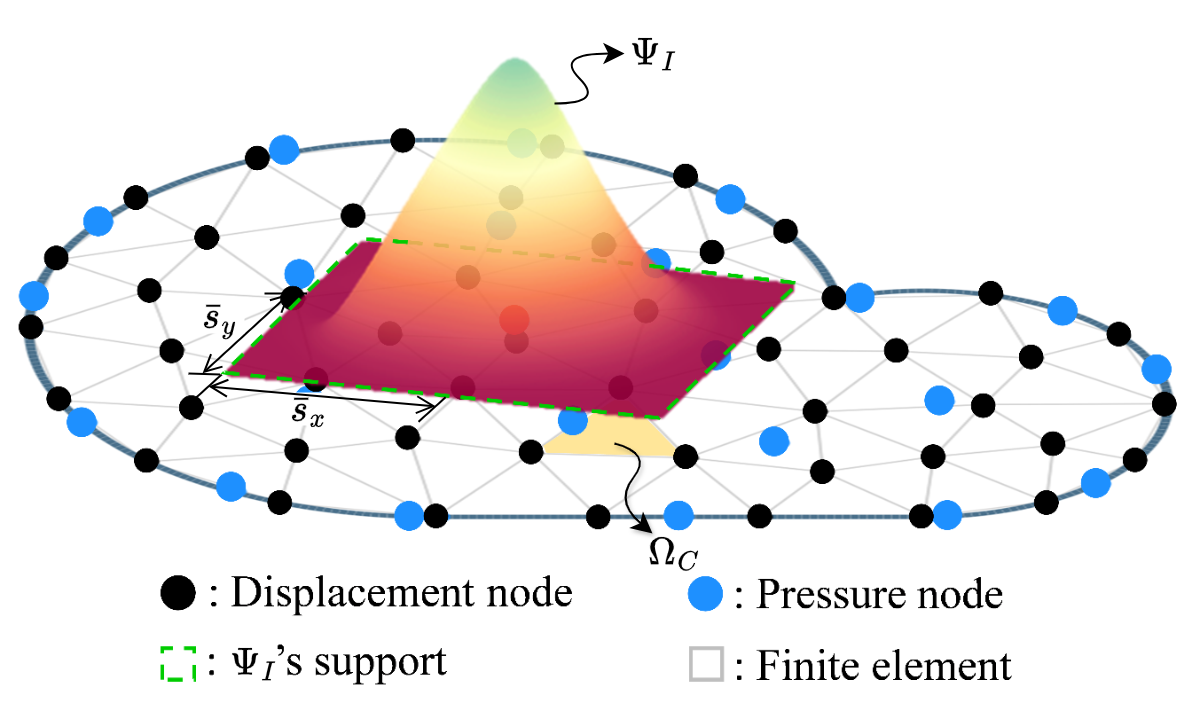
\includegraphics[width=\textwidth]{mix.png}
\caption{Illustration for reproducing kernel meshfree approximation}\label{fg:rk_approximation}
\end{figure}

\subsection{Pressure node distributions with optimal constraint ratio}\label{subsec:optimal_constraint_ratio}

In this subsection, 2D and 3D inf-sup tests \cite{chapelle1993}, as defined in Eq. \ref{infsup_test}, are conducted using the mixed FE-meshfree formulations to validate the proposed inf-sup value estimator.
The 2D test considers the square domain $\Omega = (0,1)\times (0,1)$, where the displacement is discretized by Tri3 and Quad4 with $4\times 4$, $8\times 8$, $16\times 16$ and $32\times 32$ elements, Tri6 and Quad8 with $2\times 2$, $4\times 4$, $8\times 8$ and $16\times 16$ elements, respectively. The 3D test employs a cube domain $\Omega = (0,1)\times (0,1)\times (0,1)$ with $4\times 4$, $8\times 8$ and $16\times 16$ elements for the Tet4 and Hex8.
For pressure discretization, linear meshfree approximation with a normalized support size of $1.5$ is employed for Tri3, Quad4, Tet4 and Hex8.
For Tri6 and Quad8, a quadratic meshfree approximation with a normalized support size of $2.5$ is utilized.
In order to avoid the influence of interpolation error, uniform nodal distributions are used for pressure discretizations, for example in Figure \ref{fg:infsup_mesh}, which displays $4\times4$ Quad4 elements with $4\times3$ uniformly distributed pressure nodes.

\begin{figure}[H]
\centering
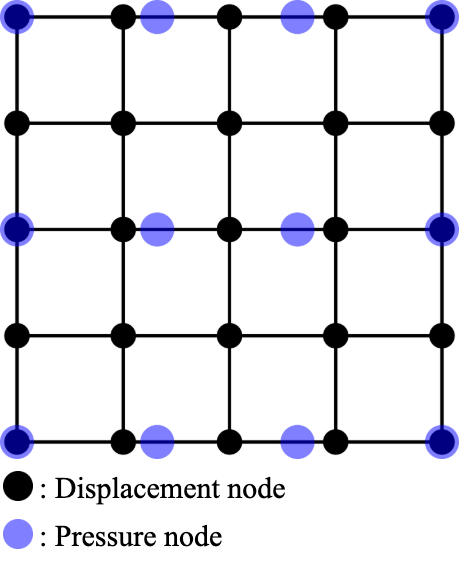
\includegraphics[width=0.5\textwidth]{infsup_mesh.png}
\caption{Illustration of uniform nodal distribution for inf--sup test with $n_u=5\times5$, $n_p=4\times3$}\label{fg:infsup_mesh}
\end{figure}

Figures \ref{fg:infsup_convergence_2D_a}--\ref{fg:infsup_convergence_3D_b} show the corresponding results, in which the red line stands for the value of $\beta$ with respect to the number of pressure nodes $n_p$, and the vertical dashed line denotes the stabilized number $n_s$. The deeper color of the lines means mesh refinement. The results show that, no matter linear or quadratic elements, as $n_p$ increases over $n_s$, the value of $\beta$ sharply decreases, and then the inf-sup condition cannot be maintained. This result is consistent with the discussion in Section \ref{sec:constraint_ratio}, and again verifies the effect of the proposed estimator.

Moreover, the mixed formulation's results with the traditional optimal constraint ratio $r=n_d$ are listed in these figures as well, and $\beta$ in this circumstance is already much smaller than those in the optimal range. Considering the results shown above, the easy programming and efficiency, the pressure nodes are chosen among the displacement nodes.
The optimal schemes for linear and quadratic, 2D and 3D element discretizations, namely with $r=r_{opt}$, are shown in Figure \ref{fg:mix_scheme},
where every other displacement node is selected as the pressure node.
For practical implementations of linear cases, the pressure nodes are initially generated using traditional approaches, such as Delaunay triangulation.
Subsequently, the displacement nodes are then obtained through a standard mesh refinement process to the pressure nodes.
For quadratic approximations in Tri6 and Quad8 elements, the element vertices are chosen as pressure nodes after displacement element generation.
Consequently, all constraint ratios evaluated using the discretizations in Figure \ref{fg:mix_scheme} fall within the optimal range.
The corresponding inf--sup test results for these schemes are also marked in inf--sup test figure and show that, with mesh refinement, their $\beta$'s are always maintained at a non-negligible level.

\begin{figure}[H]
\centering
\includegraphics[width=\textwidth]{tri3.png}
\caption{Inf--sup test for Tri3--RK}\label{fg:infsup_convergence_2D_a}
\end{figure}

\begin{figure}[H]
\centering
\includegraphics[width=\textwidth]{tri6.png}\caption{Inf--sup test for Tri6--RK}\label{fg:infsup_convergence_2D_b}
\end{figure}

\begin{figure}[H]
\centering
\includegraphics[width=\textwidth]{quad4.png}\caption{Inf--sup test for Quad4--RK}\label{fg:infsup_convergence_2D_c}
\end{figure}

\begin{figure}[H]
\centering
\includegraphics[width=\textwidth]{quad8.png}\caption{Inf--sup test for Quad8--RK}\label{fg:infsup_convergence_2D_d}
\end{figure}

\begin{figure}[H]
\centering
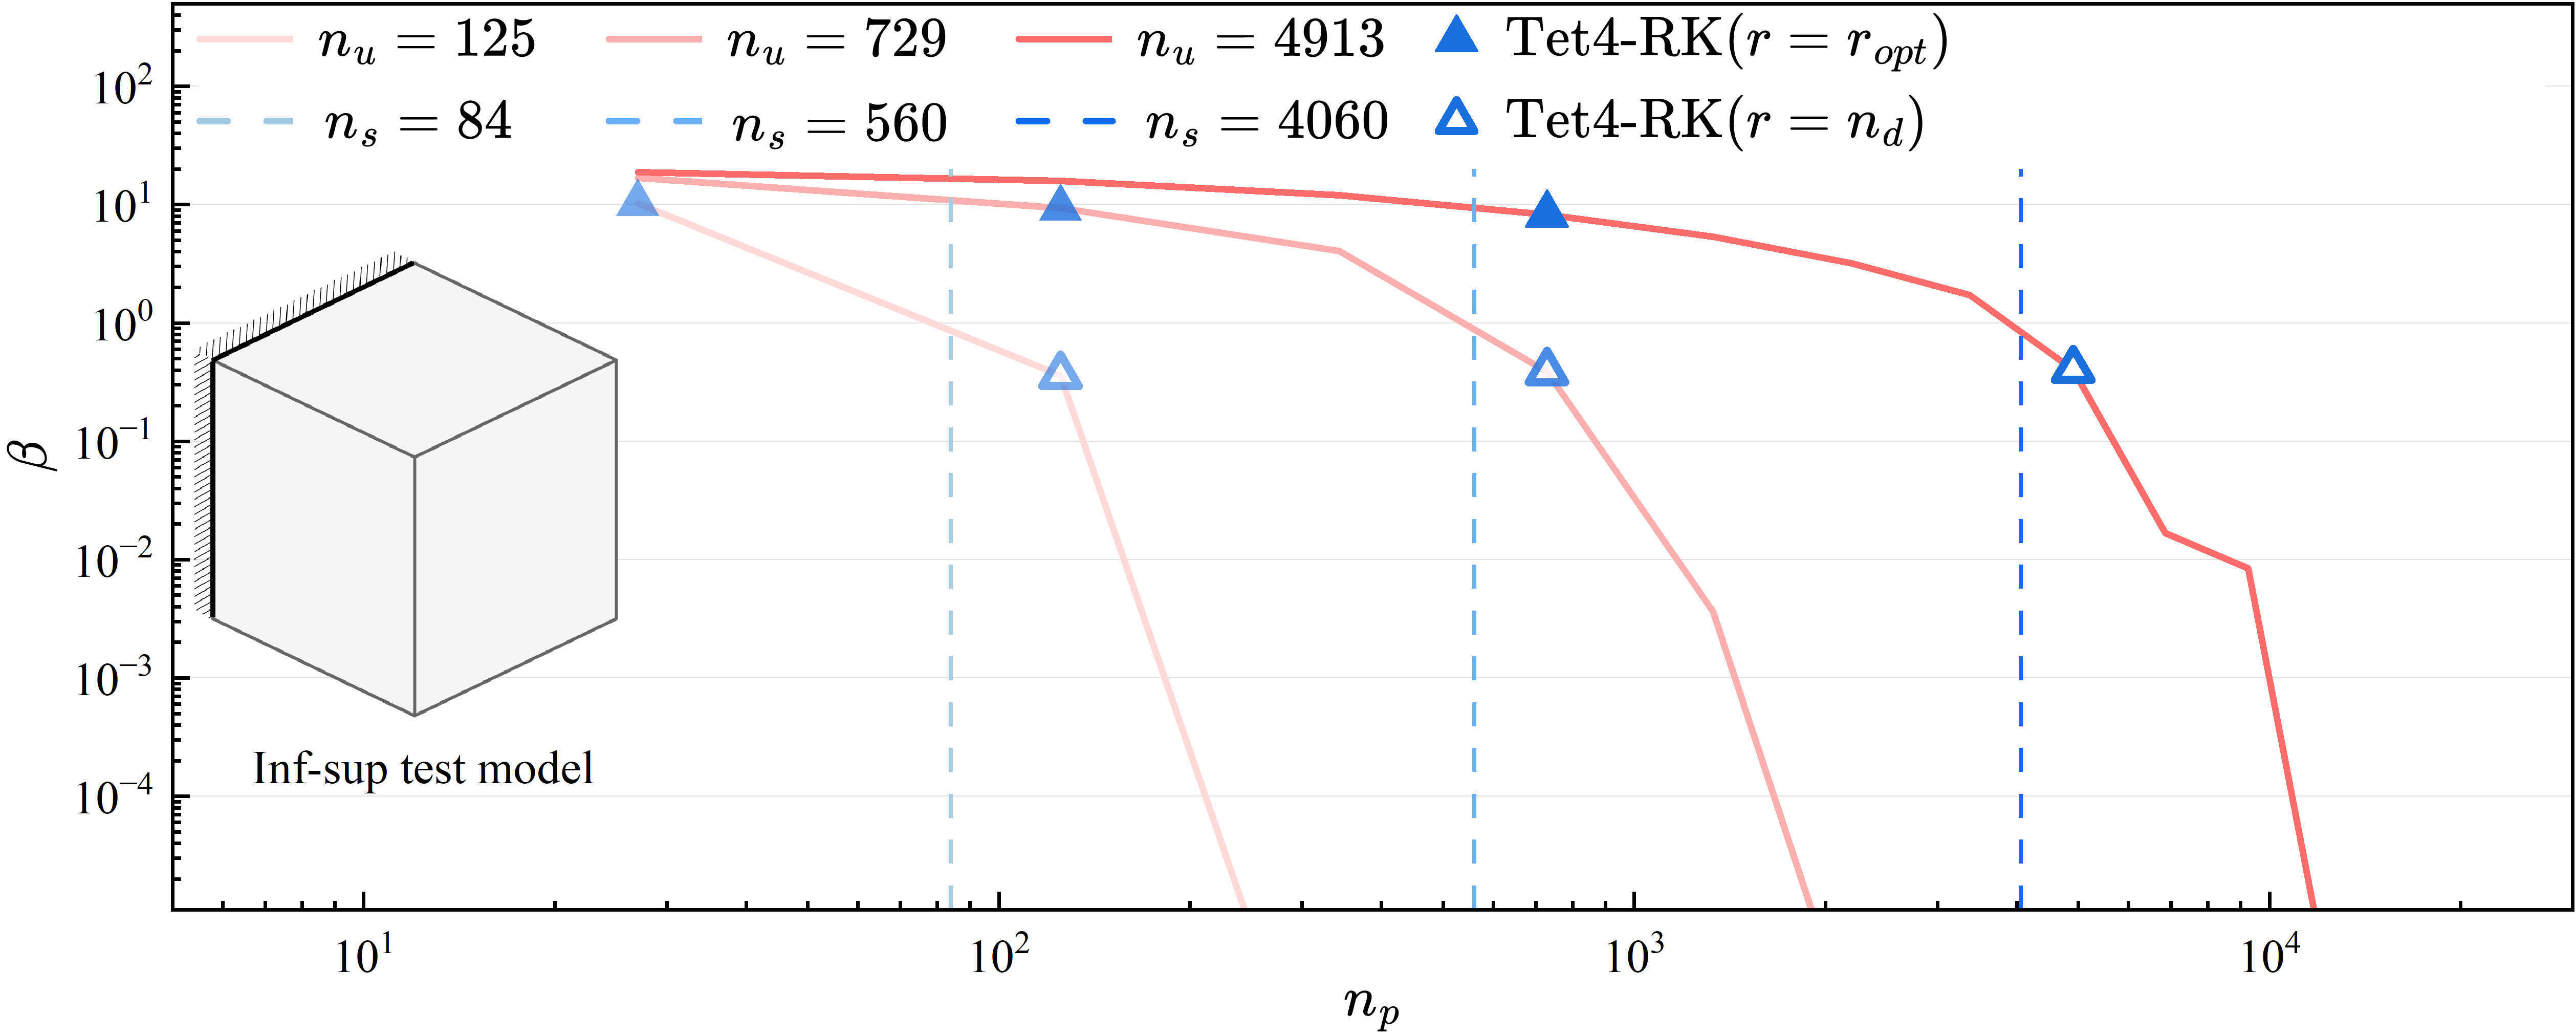
\includegraphics[width=\textwidth]{Tet4.png}\caption{Inf--sup test for Tet4--RK}\label{fg:infsup_convergence_3D_a}
\end{figure}

\begin{figure}[H]
\centering
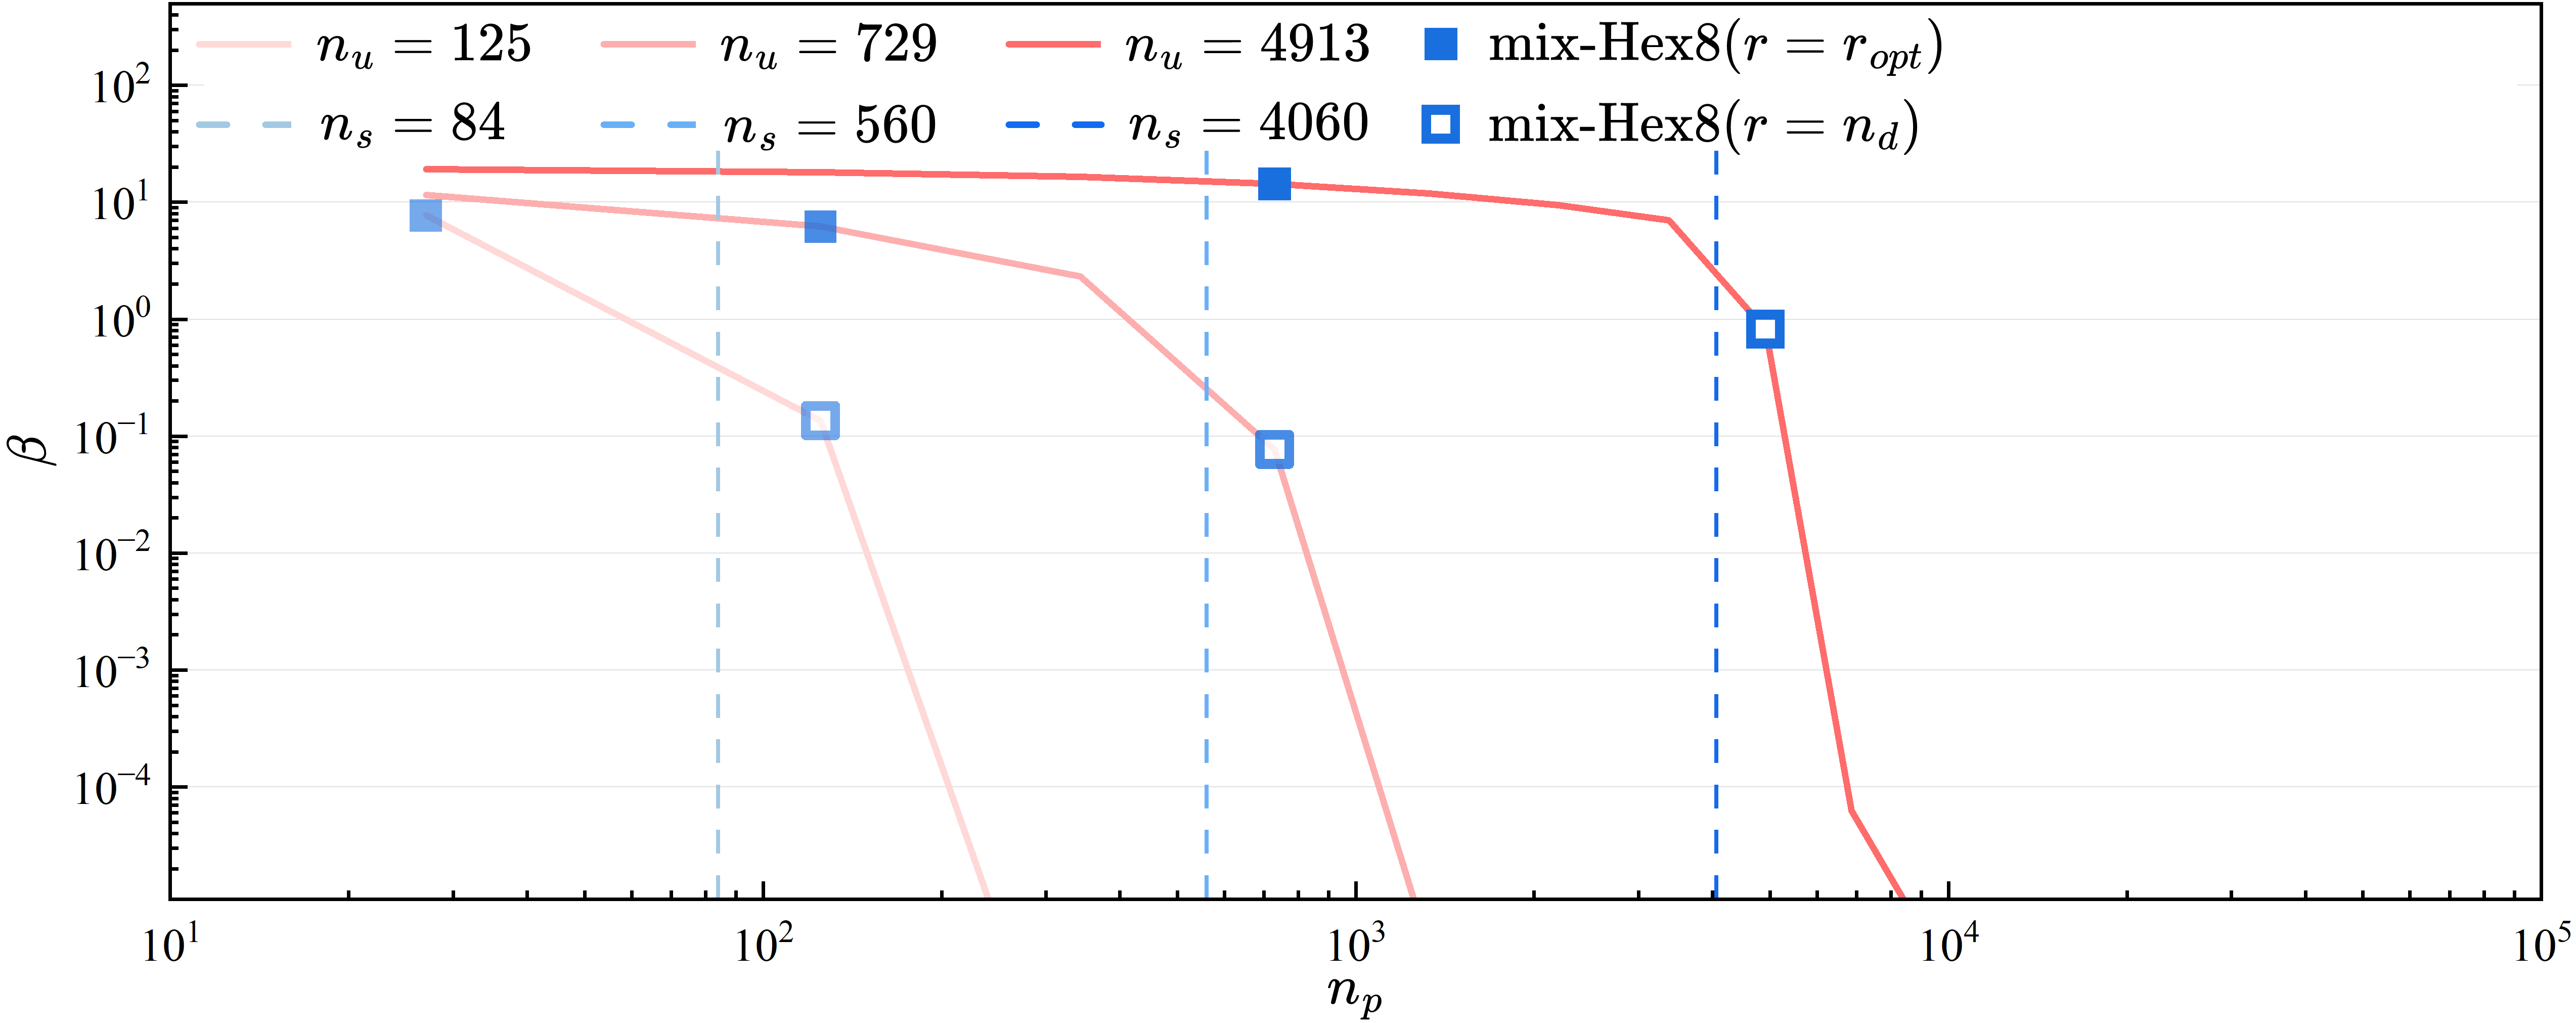
\includegraphics[width=\textwidth]{Hex8.png}\caption{Inf--sup test for Hex8--RK}\label{fg:infsup_convergence_3D_b}
\end{figure}

\begin{figure}[H]
\centering
\begin{tabular}{c@{\hspace{24pt}}c}
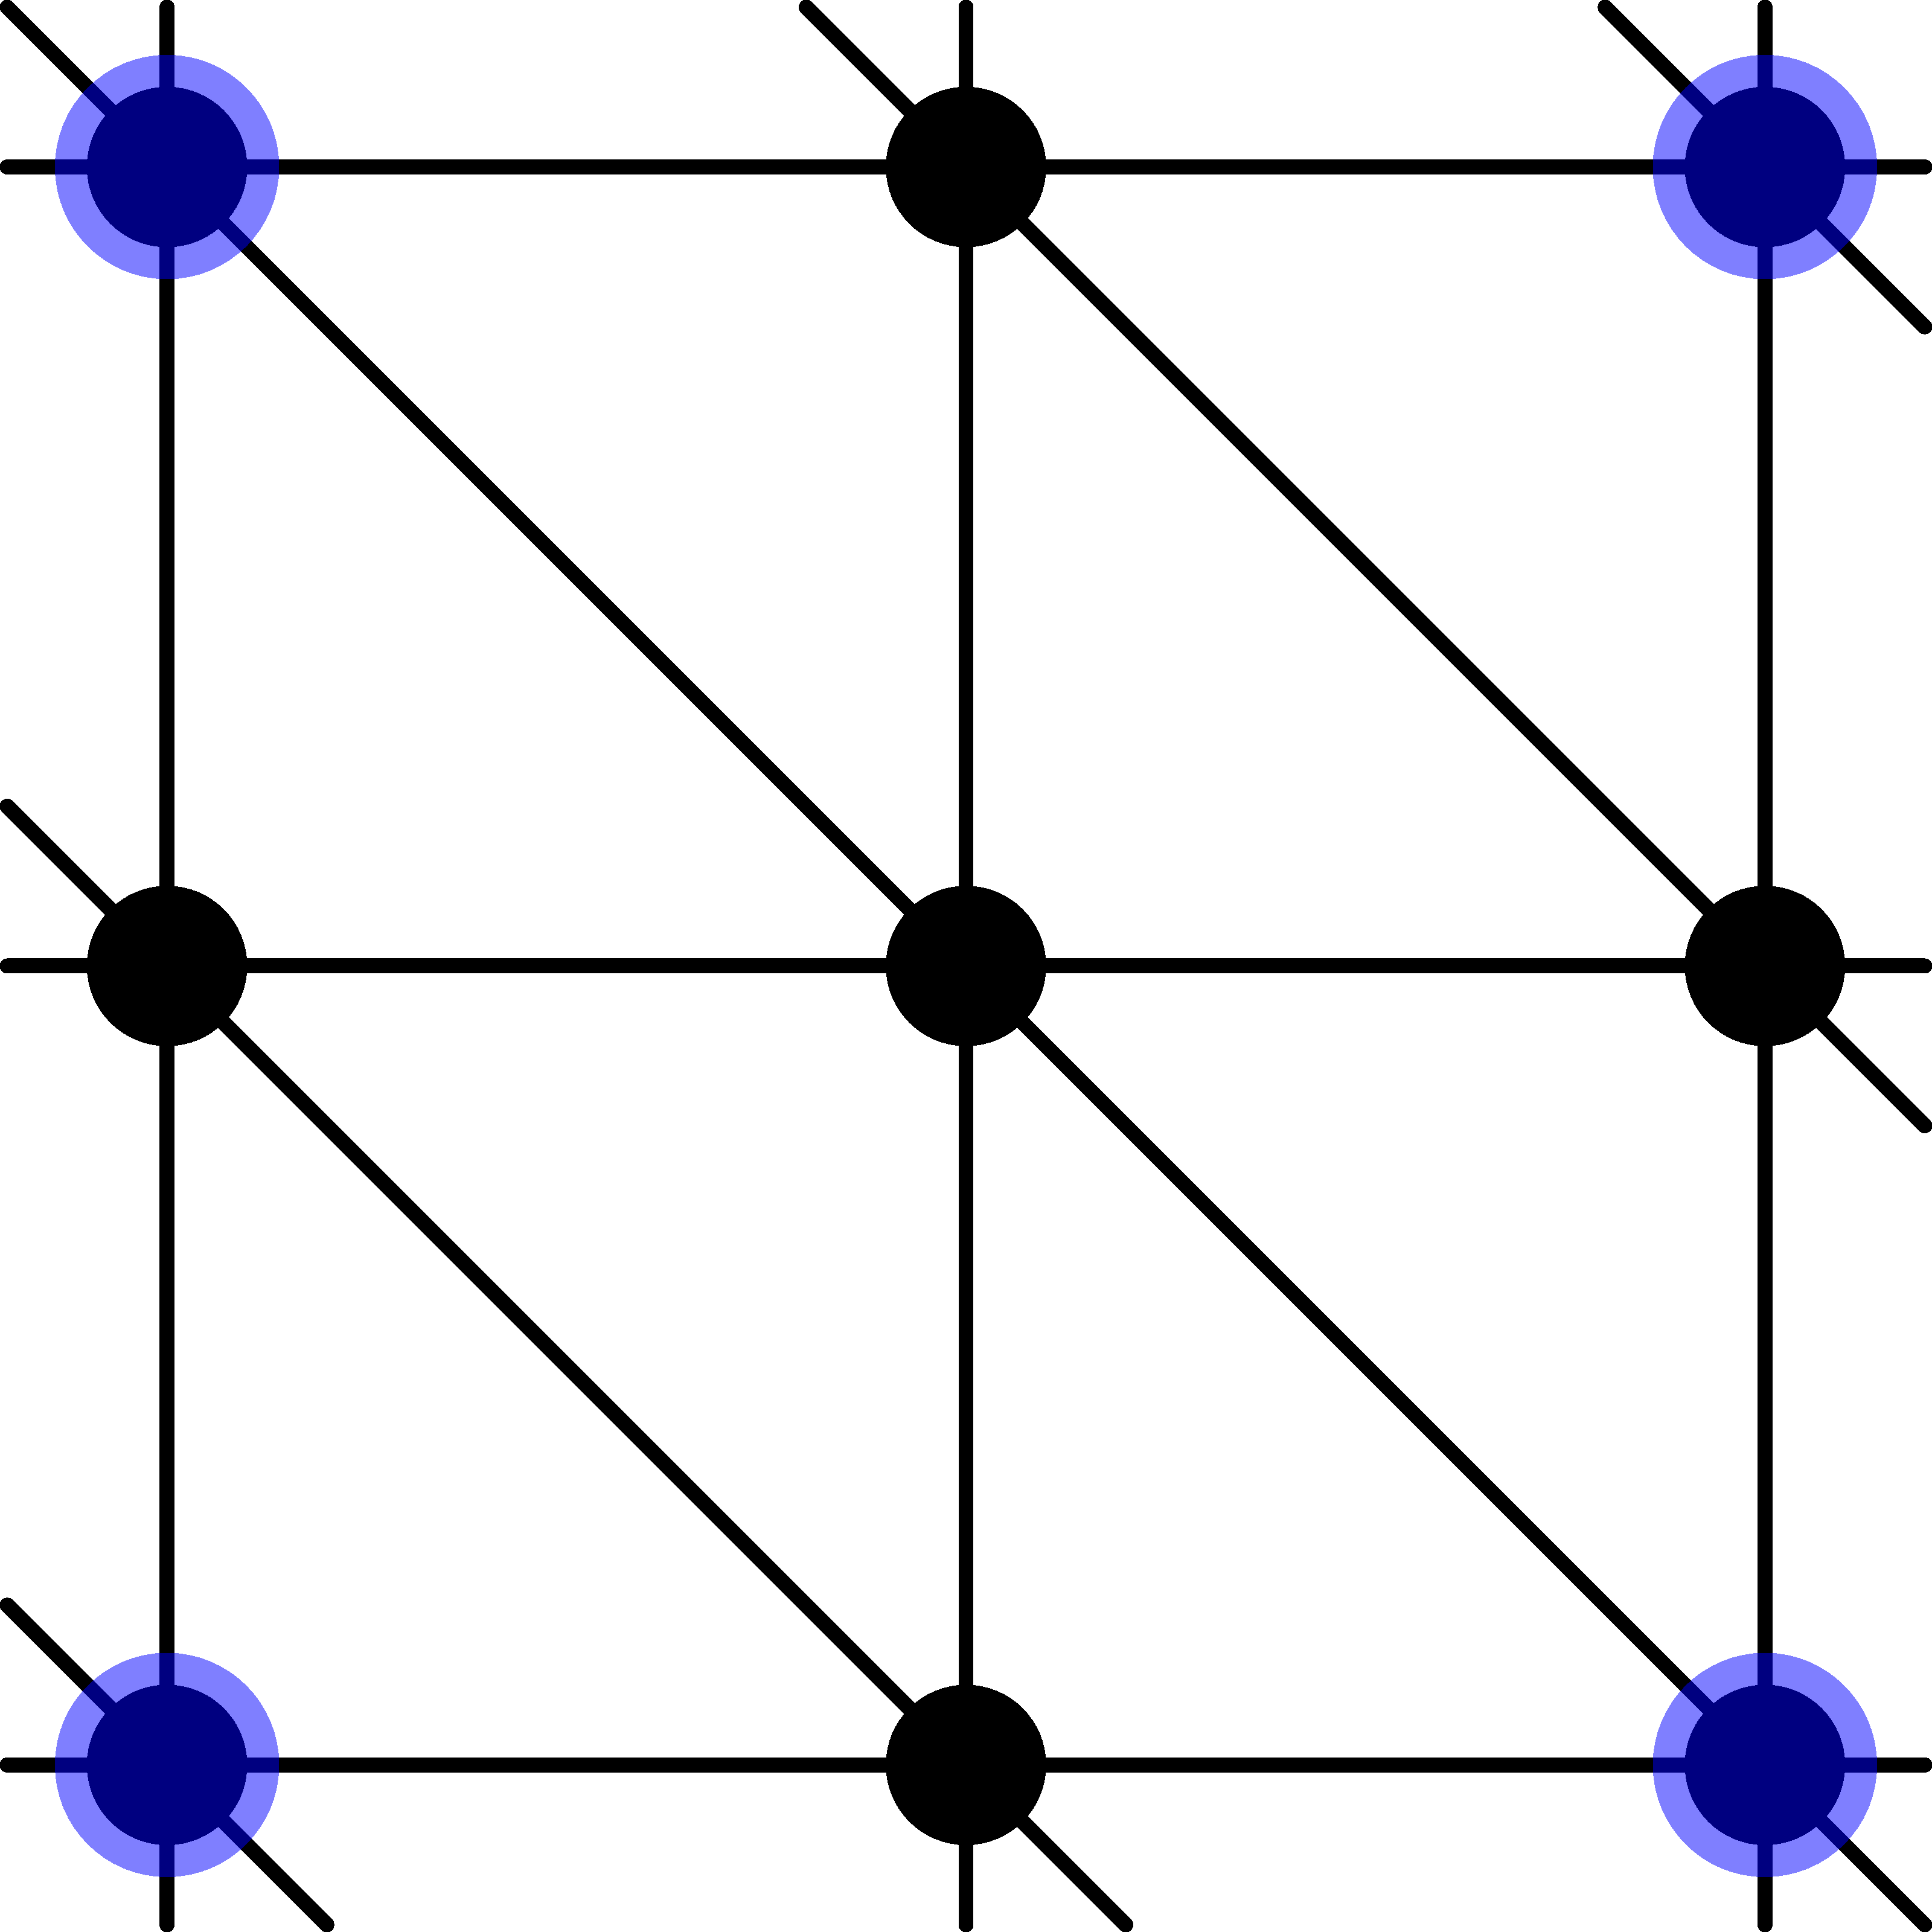
\includegraphics[width=0.28\textwidth]{mix_tri3.png} &
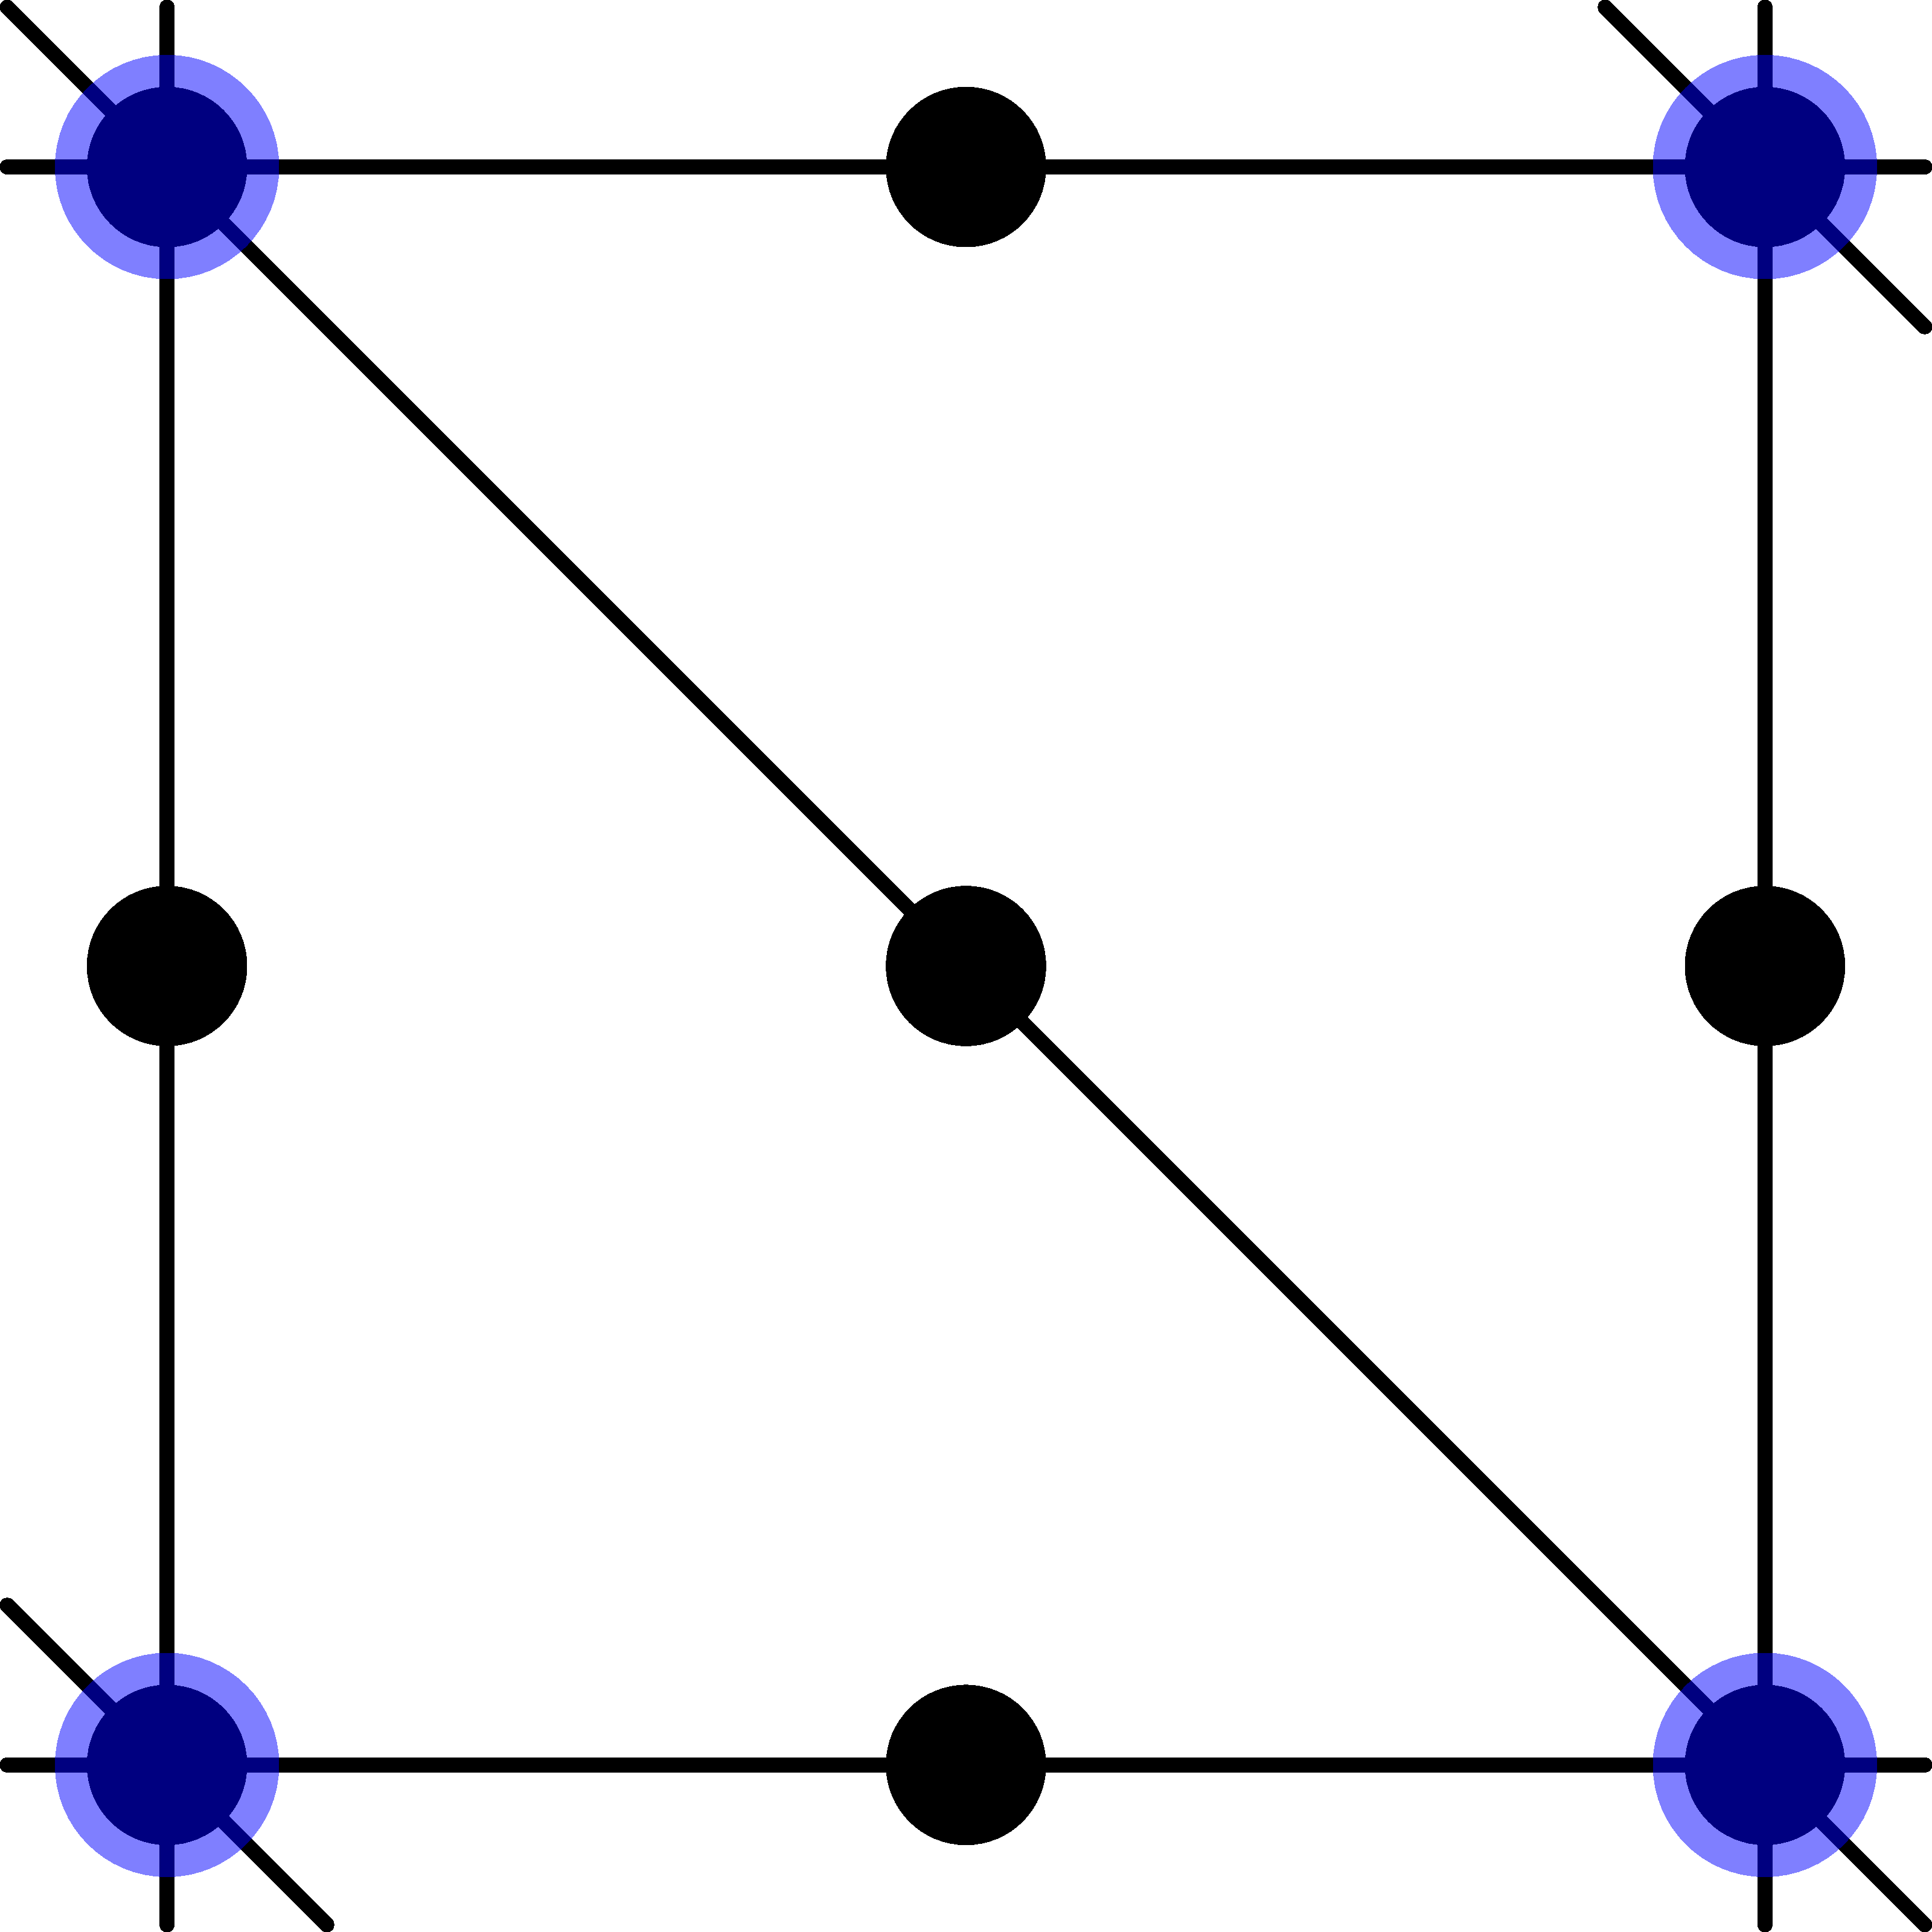
\includegraphics[width=0.28\textwidth]{mix_tri6.png} \\
Tri3--RK & Tri6--RK \\
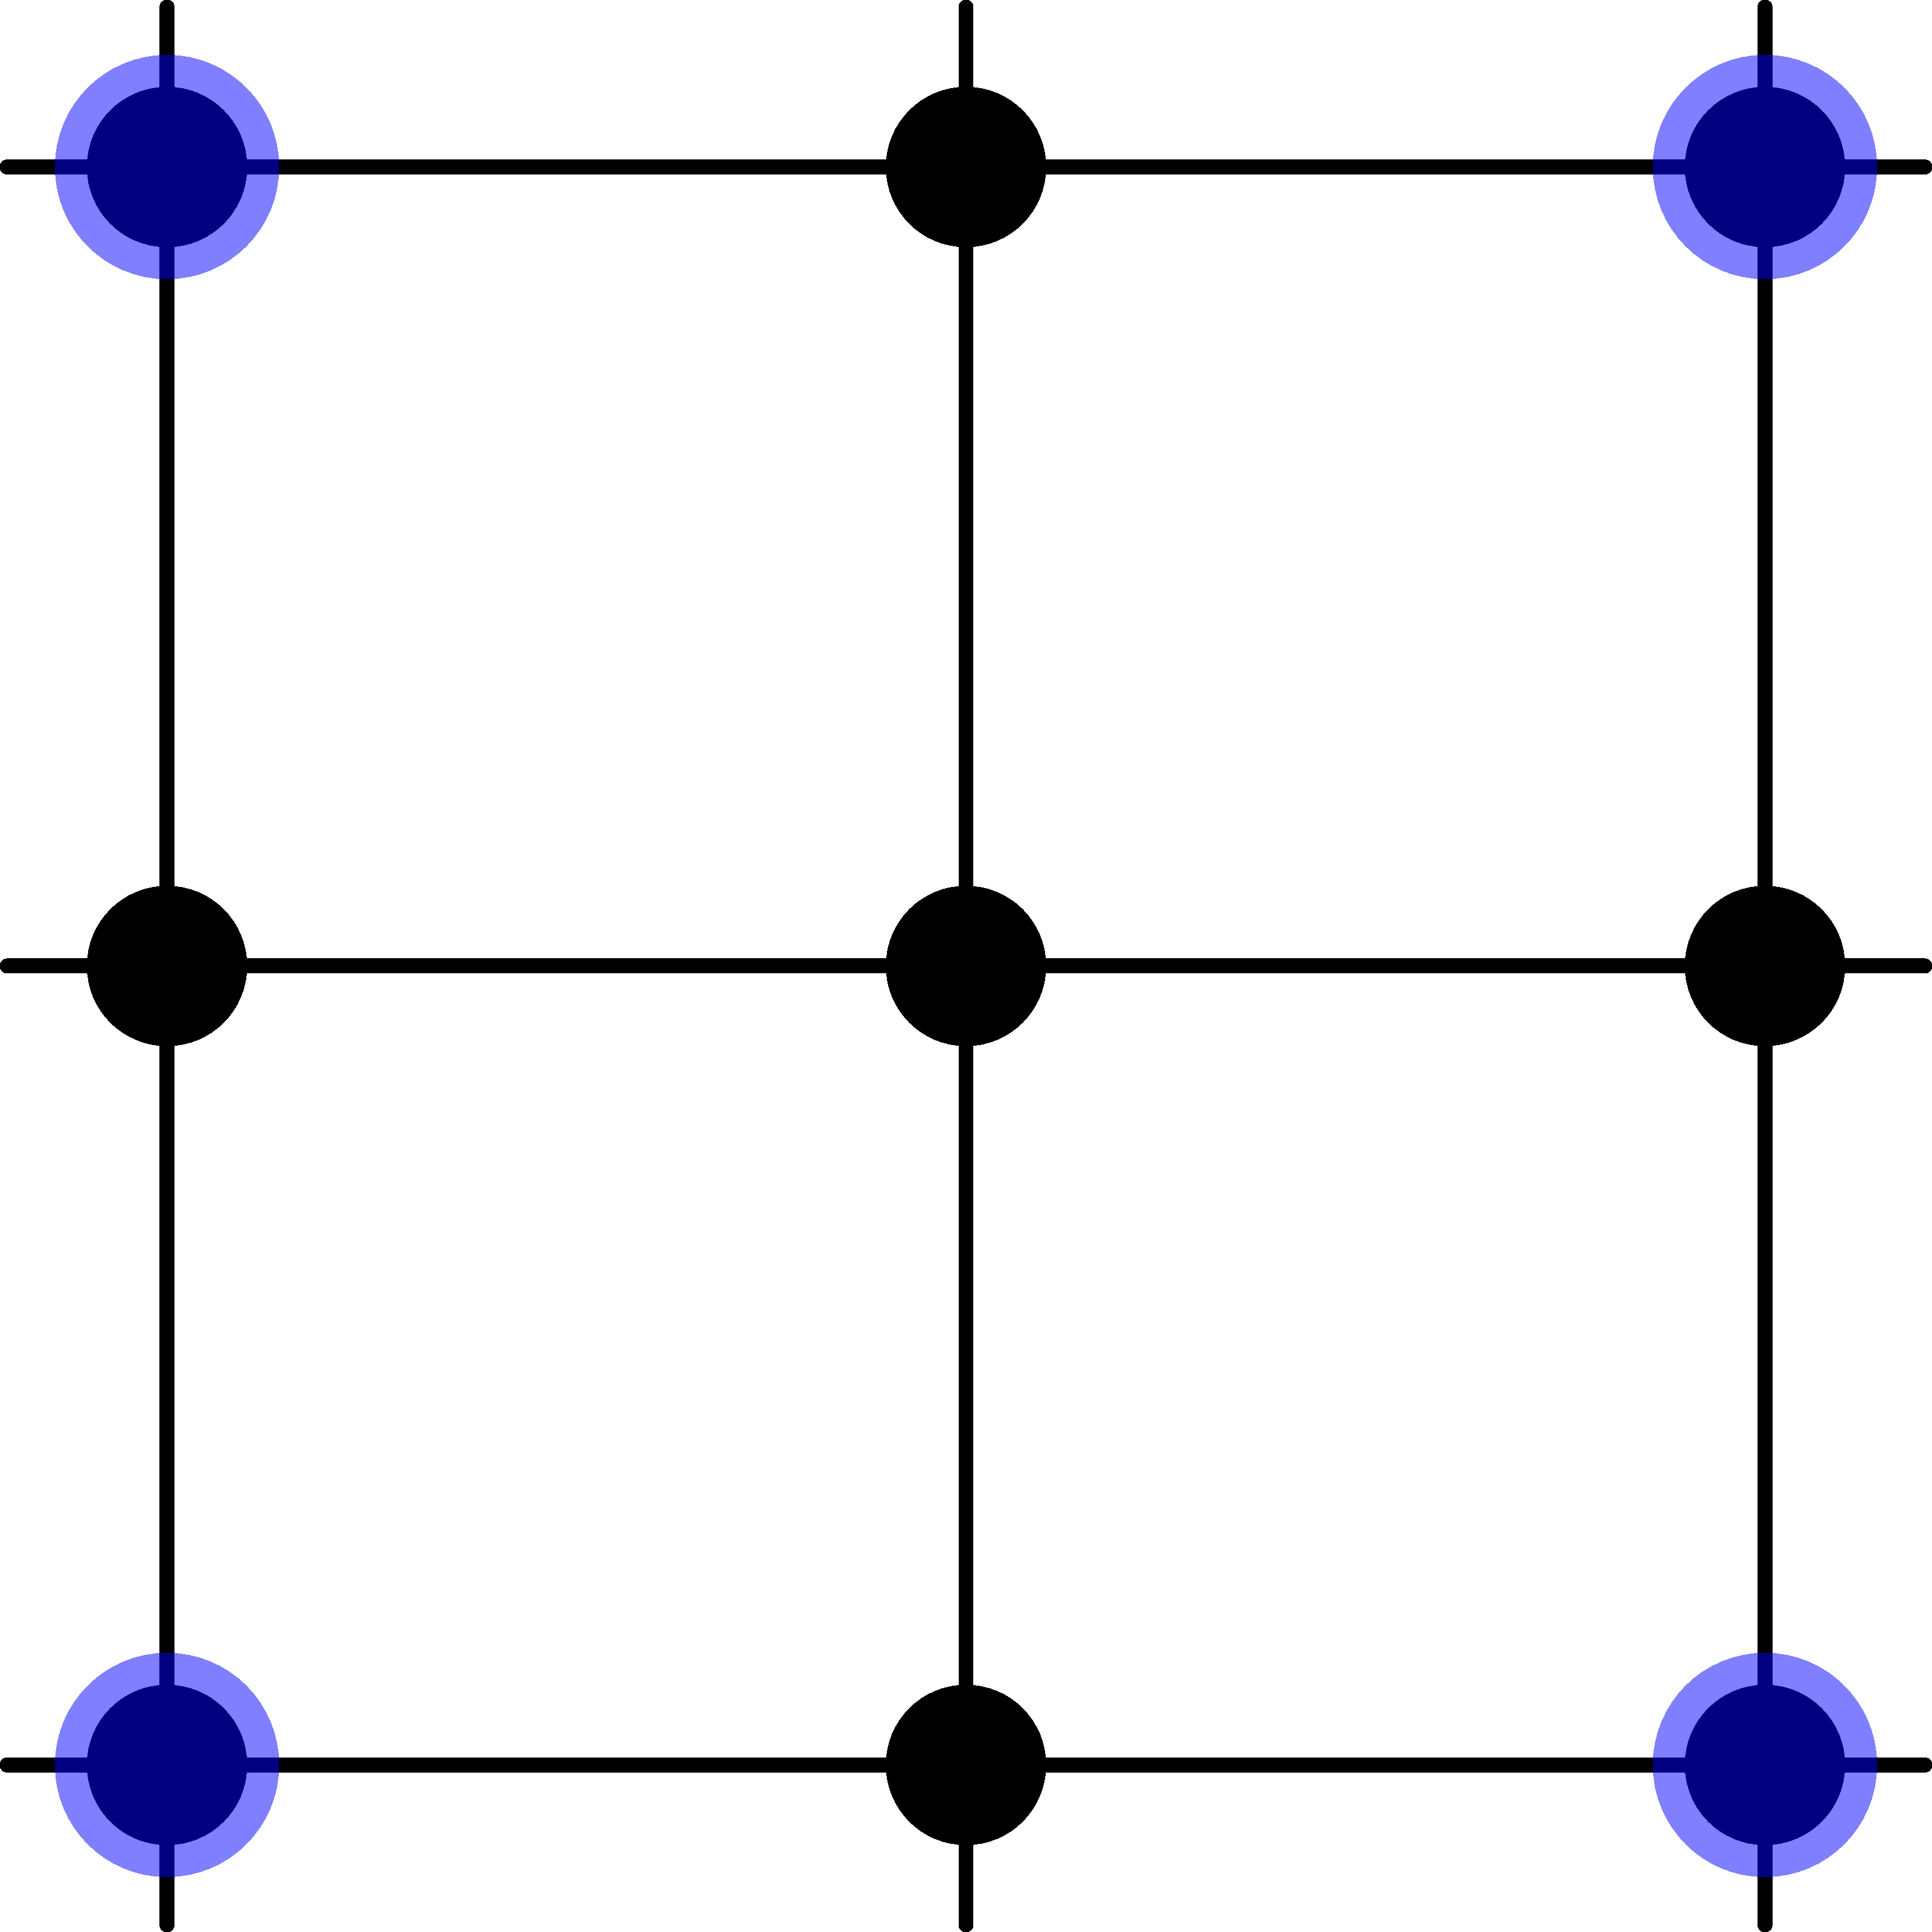
\includegraphics[width=0.28\textwidth]{mix_quad4.png} &
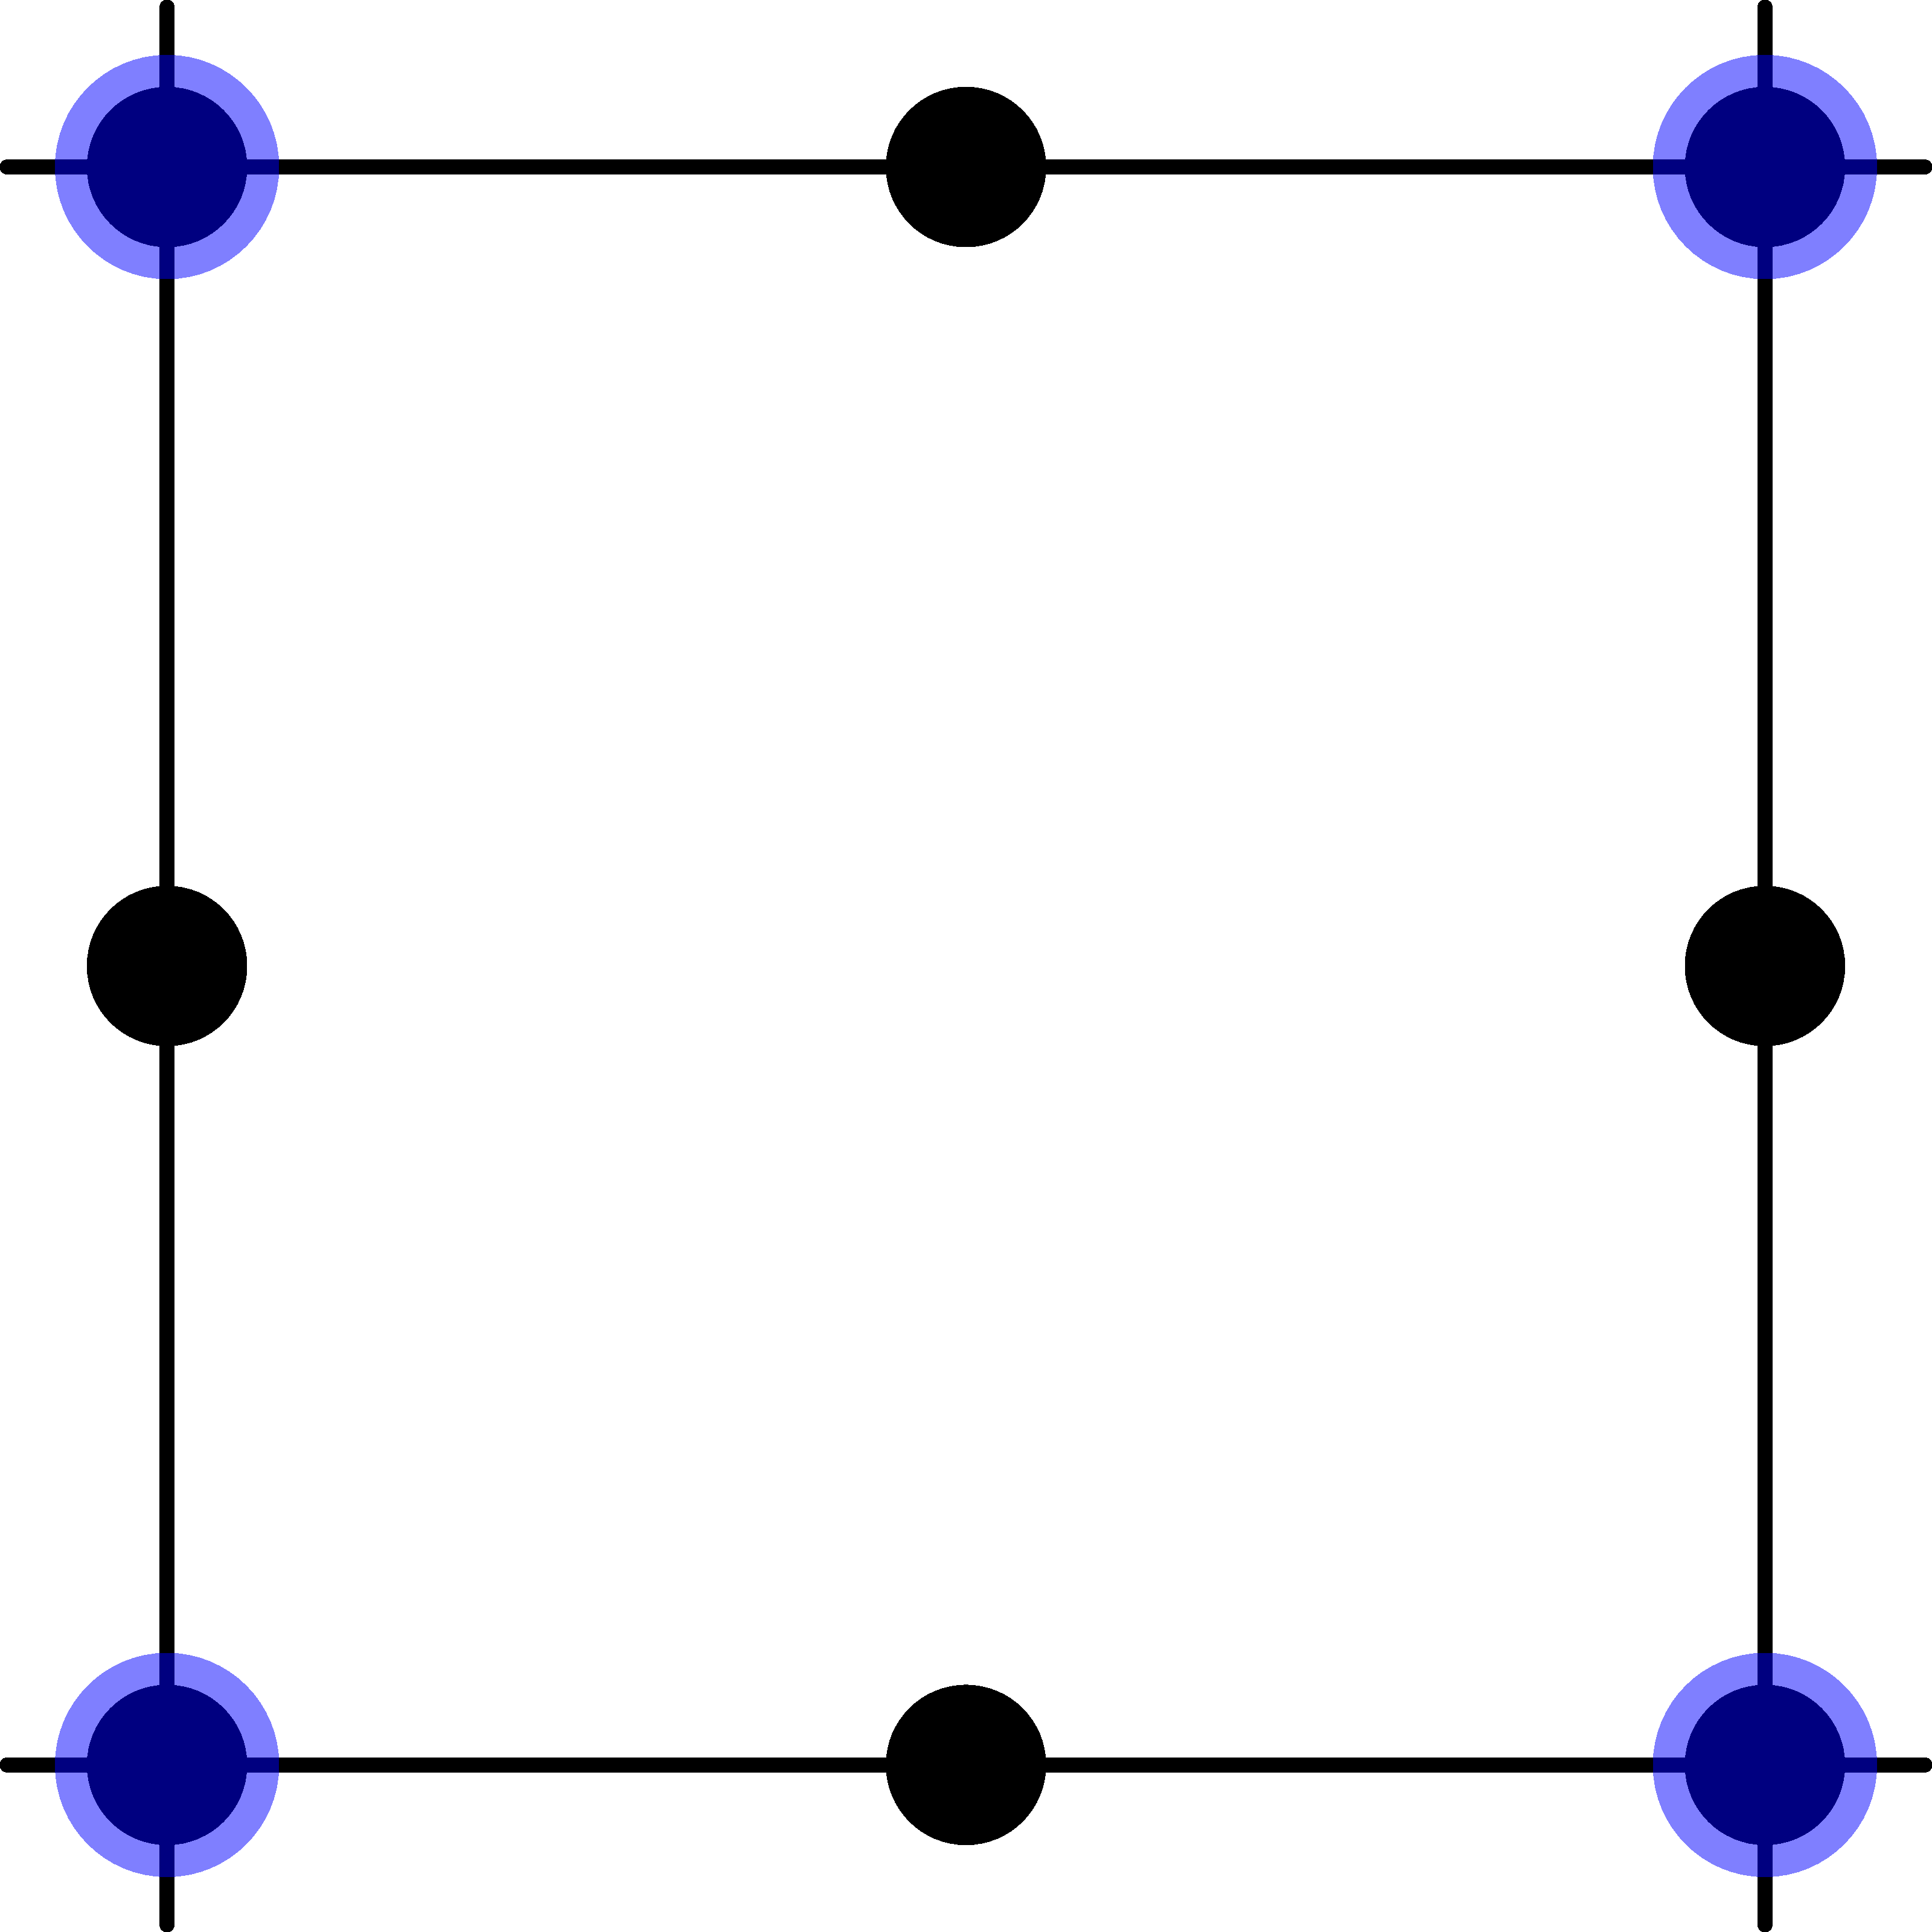
\includegraphics[width=0.28\textwidth]{mix_quad8.png} \\
Quad4--RK & Quad8--RK \\
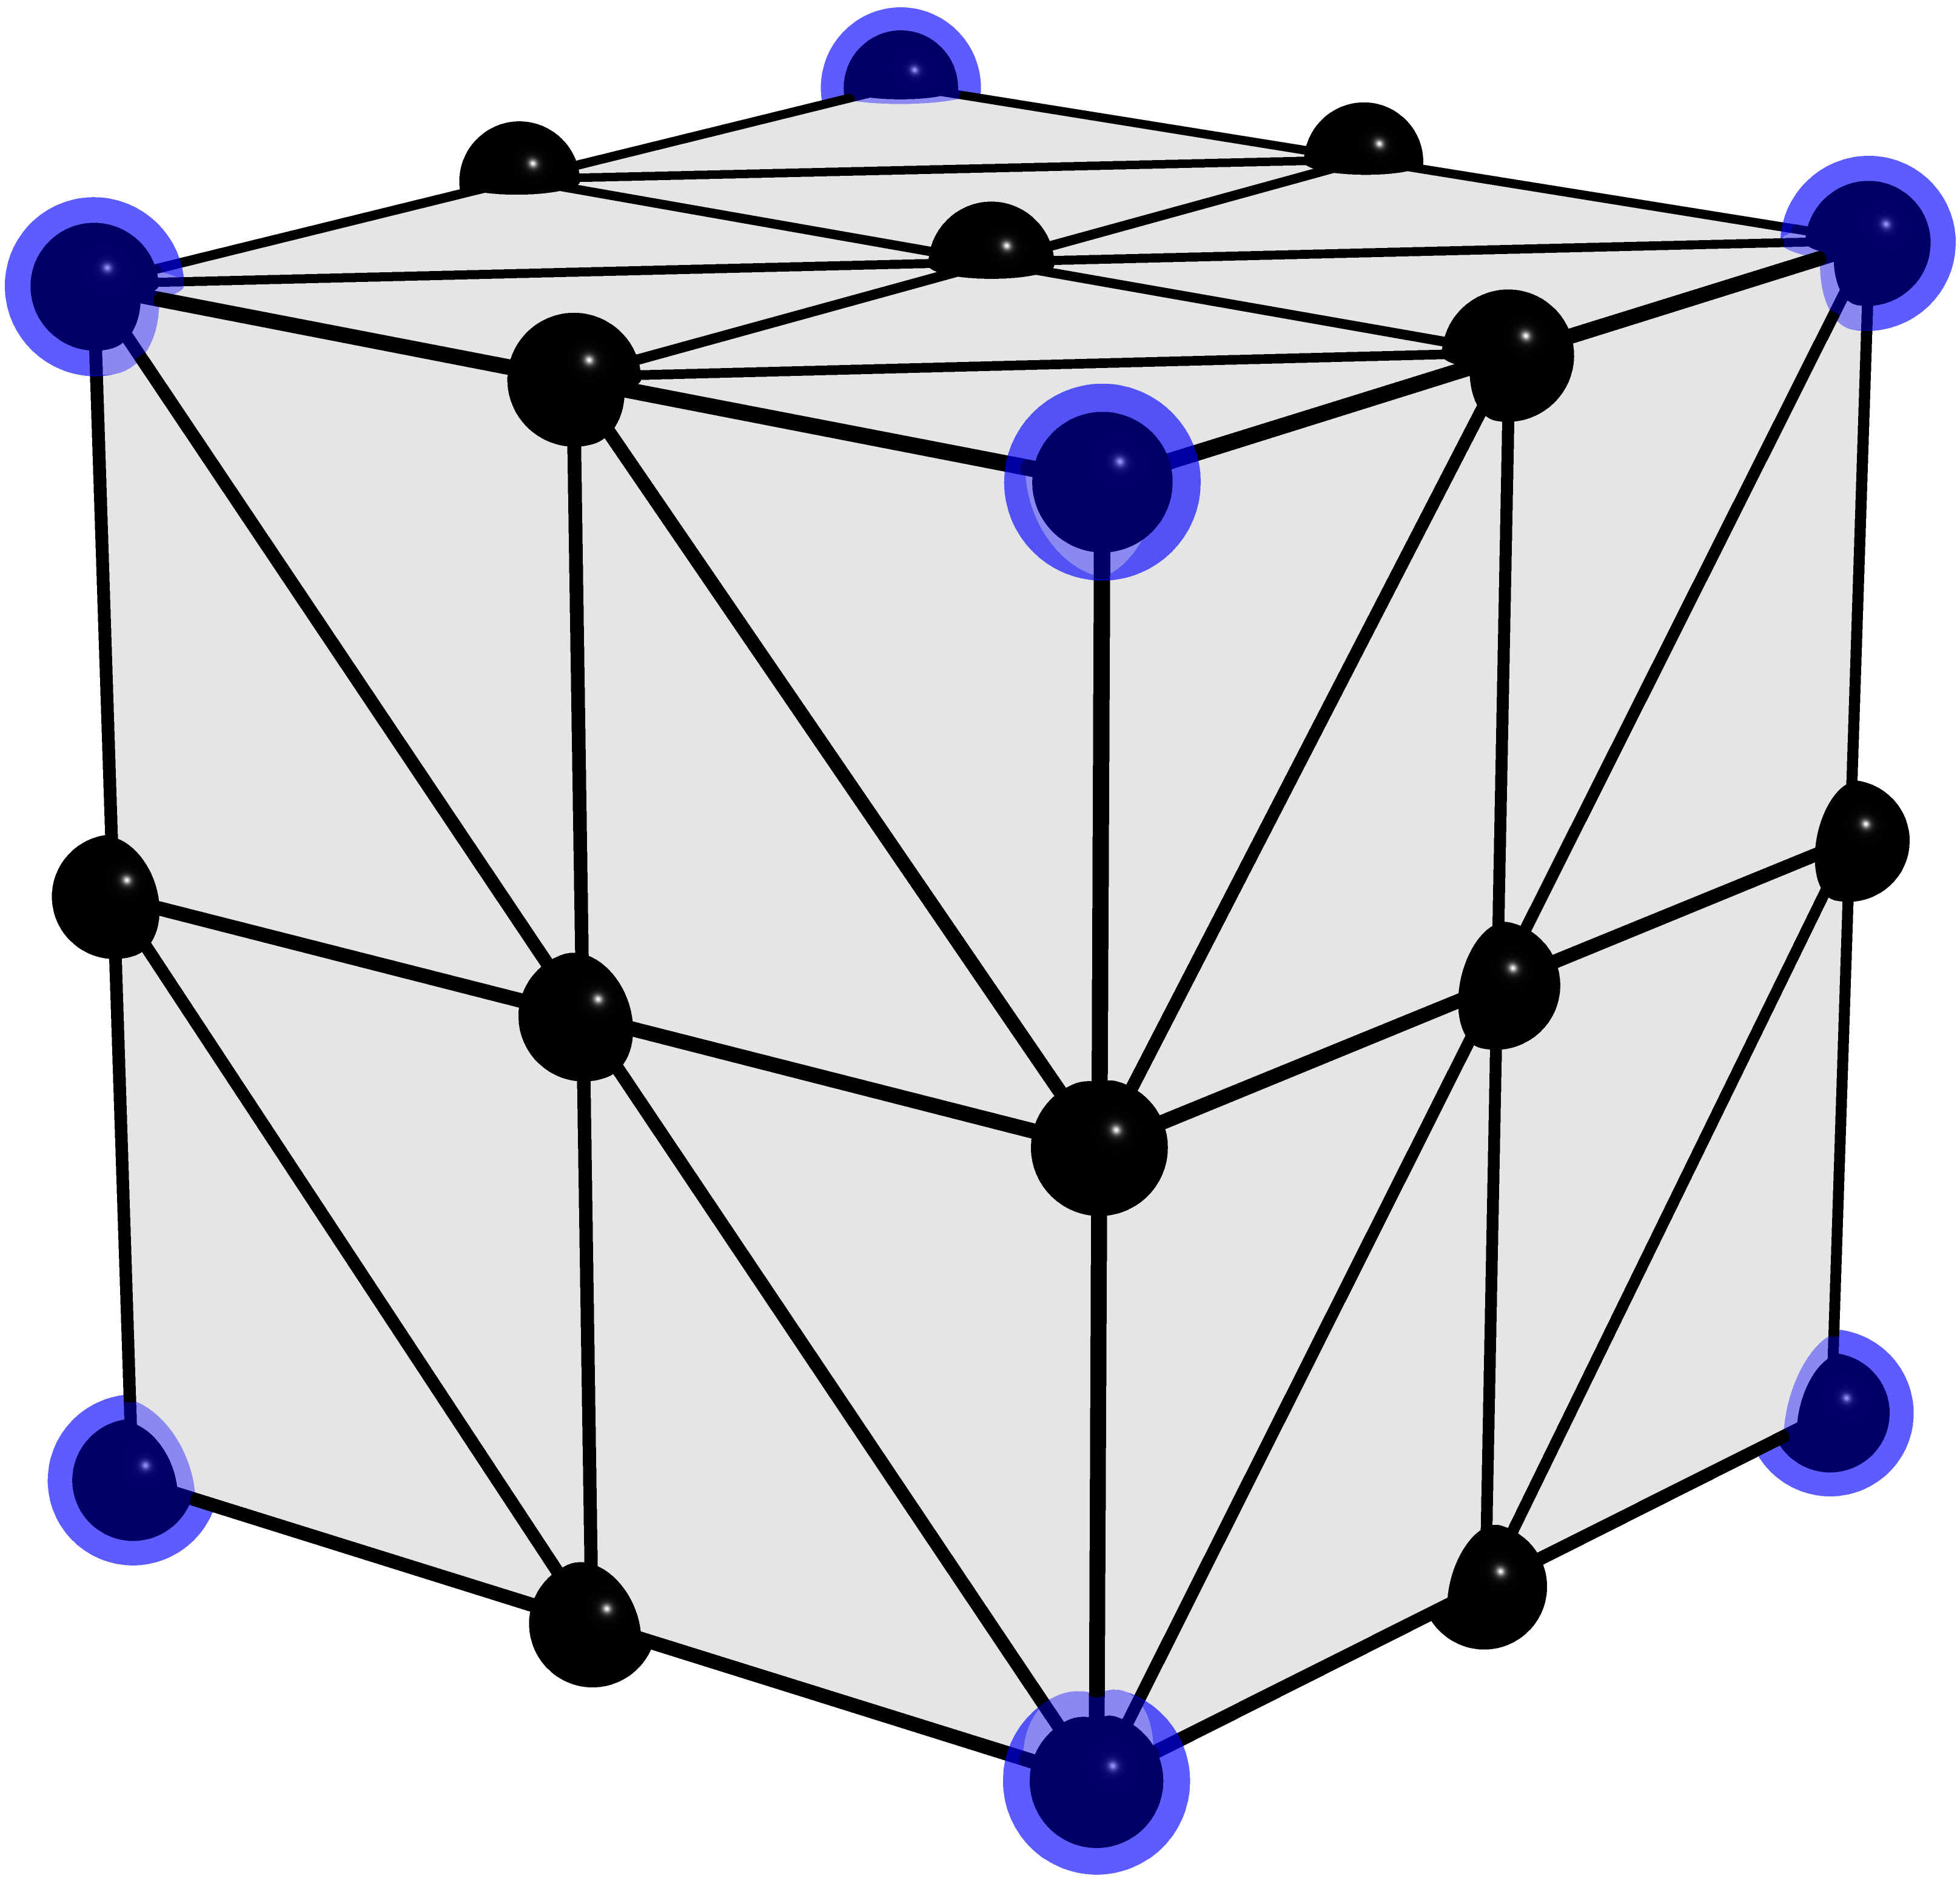
\includegraphics[width=0.28\textwidth]{mix_tet4.png} &
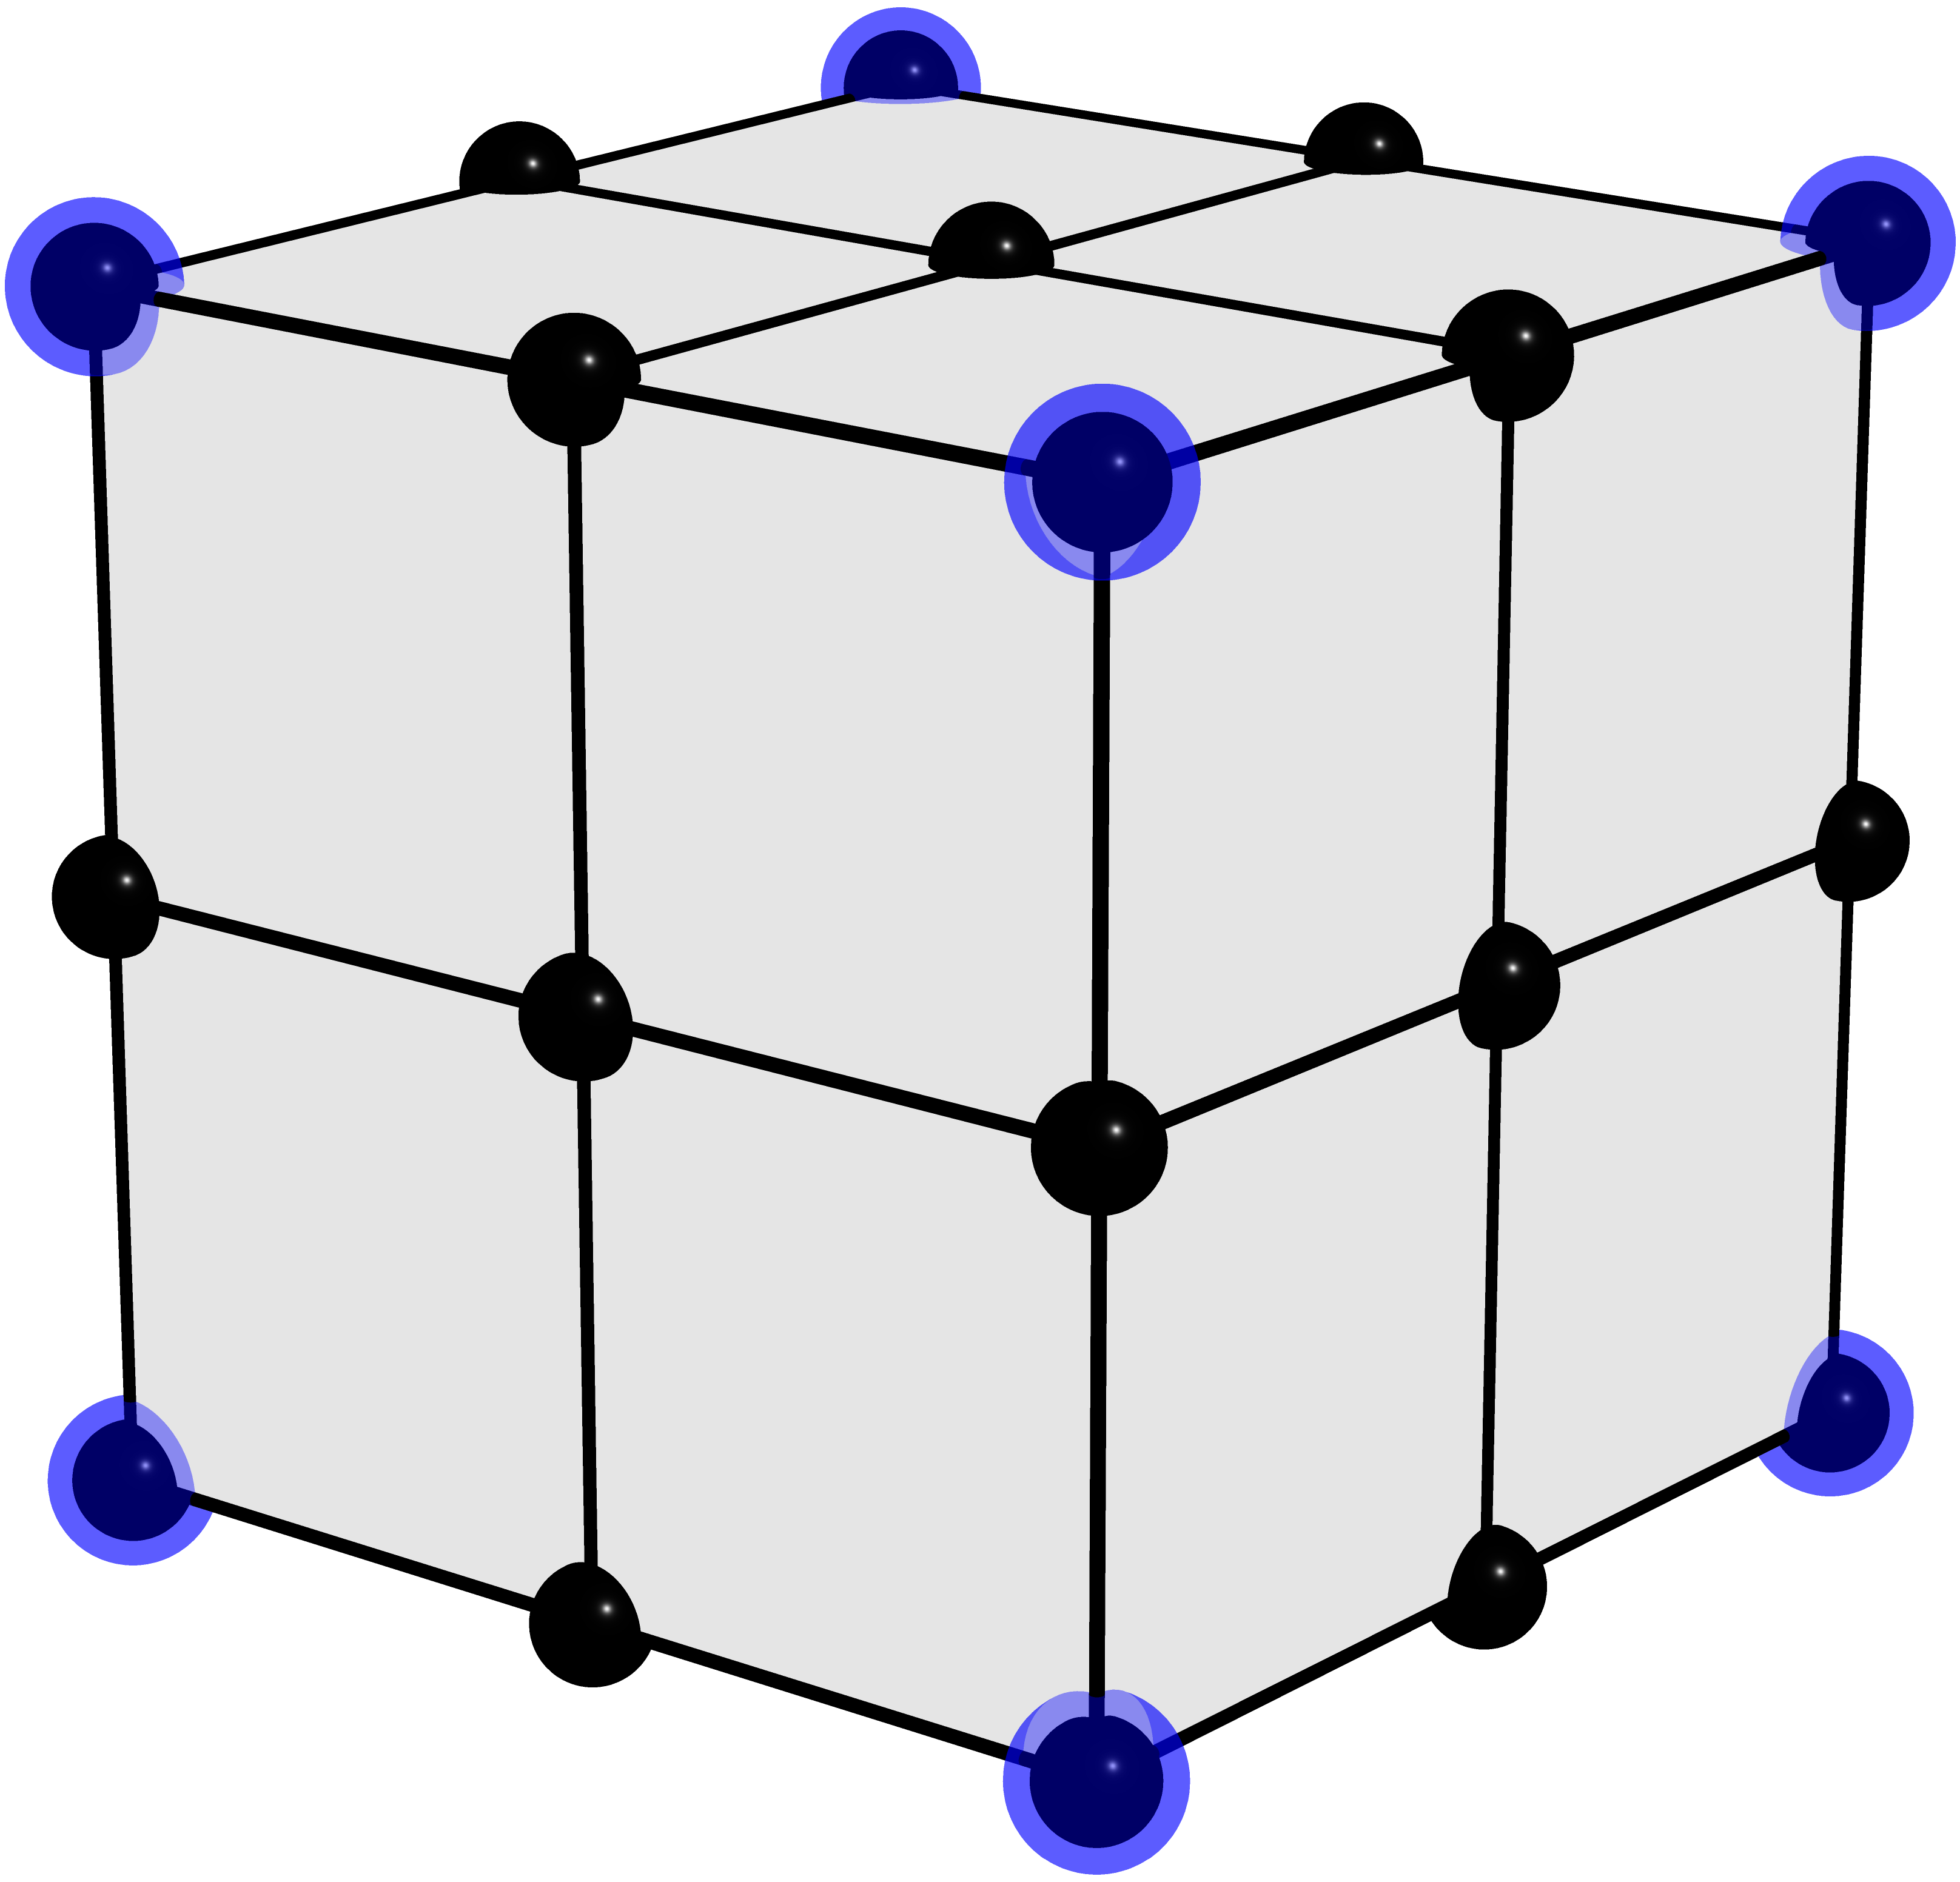
\includegraphics[width=0.28\textwidth]{mix_hex8.png} \\
Tet4--RK & Hex8--RK \\
\raisebox{-0.3\height}{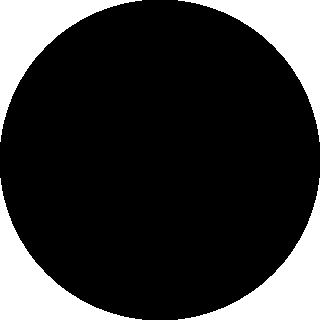
\includegraphics[width=12pt]{legend_u.png}} :Displacement node &
\raisebox{-0.3\height}{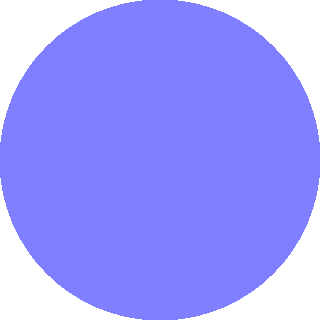
\includegraphics[width=12pt]{legend_p.png}} :Pressure node
\end{tabular}
\caption{Nodal distribution schemes for mixed FE-meshfree formulations with $r = r_{opt}$}\label{fg:mix_scheme}

\end{figure}


\section{Numerical examples}
% % \subsection{Cantilever beam problem}\label{sec:cantilever}
% Consider the cantilever beam problem shown in Figure \ref{fg:cantilever_model} with length $L = 48$, width $D = 12$, 
% and the incompressible material parameters are employed with Young's modulus $E = 3\times 10^6$, Poisson's ratio $\nu = 0.5-10^{-8}$.
% The left hand side is fixed and the right side subject a concentrate force $P = 1000$.
% All the prescribed values in boundary conditions are evaluated by analytical solution that is given as follows\cite{timoshenko1969theory}:
% \begin{equation}
%     \left \{
%         \begin{aligned}
%         u_x(\boldsymbol x) &= - \frac{Py}{6\bar EI}
%         \left (
%             (6L - 3x)x + (2 + \bar \nu)(y^2 - \frac{D^2}{4})
%         \right ) \\
%         u_y(\boldsymbol x) &= \frac{Py}{6\bar EI}
%         \left (
%             3 \bar \nu y^2(L-x) + (4+5\bar \nu) \frac{D^2x}{4} + (3L-x)x^2
%         \right )
%         \end{aligned}
%     \right .
% \end{equation}
% where $I$ is the beam's moment of inertia, $\bar E$ and $\bar \nu$ are the material parameters for plane strain hypothesis, they can be expressed by:
% \begin{equation}
%     I = \frac{D^3}{12}, \quad 
%     \bar E = \frac{E}{1-\nu^2}, \quad 
%     \bar \nu = \frac{\nu}{1-\nu}
% \end{equation}
% And correspondingly, the stress components are evaluated by
% \begin{equation}
%     \left \{
%         \begin{aligned}
%             \sigma_{xx} &= - \frac{P(L-x)y}{I} \\
%             \sigma_{yy} &= 0 \\
%             \sigma_{xy} &= \frac{P}{2I}(\frac{D^2}{4}-y^2)
%         \end{aligned}
%     \right .
% \end{equation}

% \begin{figure}[H]
% \centering
% 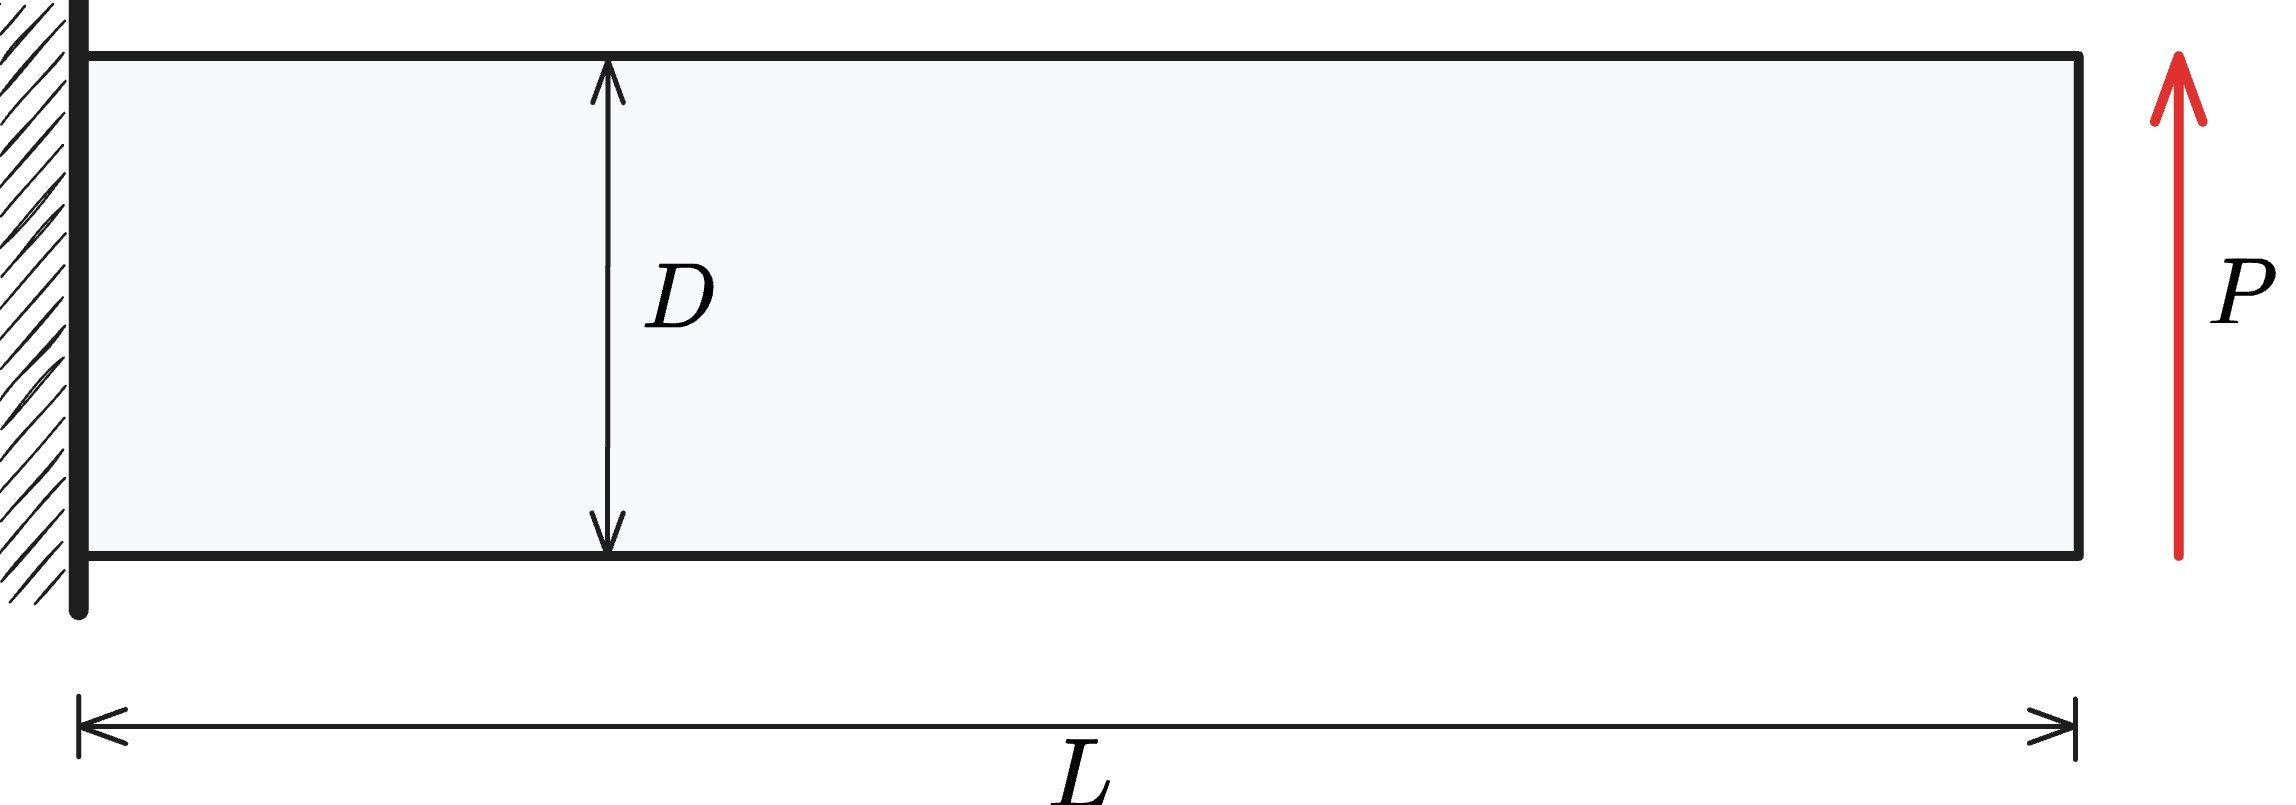
\includegraphics[width=0.7\textwidth]{png/cantilever_model.png}
% \caption{Illustration of cantilever beam problem}\label{fg:cantilever_model}
% \end{figure}

% In this problem, the Quad4 element with $16\times 4$, $32\times 8$, $64\times 16$, $128\times 32$ grids,
% and Quad8 element with $8\times 2$, $16\times 4$, $32\times 8$, $64\times 16$ grids are employed for displacement discretization.
% The pressure are discretized by linear and quadratic meshfree approximations with 1.5 and 2.5 characterized support sizes respectively.
% The strain and pressure errors respected to pressure nodes $n_p$ are displayed in Figure \ref{fg:cantilever_ns}, where the vertical dashed lines stand for the stabilized number $n_s$.
% The figure implies that, the Quad8 shows better performance than Quad4, since the Quad8's displacement results are stable no matter the constraint ratio in optimal range or not. And the Quad4's displacement errors increase as soon as the $n_p>n_s$. 
% However, both Quad4's and Quad8's pressure error immediately increase while their constraint ratios are out of optimal range,
% and Quad8 still have better results than Quad4. 
% Figure \ref{fg:cantilever_convergence}is the strain and pressure error convergence comparisons for this cantilever beam problem,
% in which, except Quad8--RK($r=2$) for strain error, all formulations with traditional constraint ratio of $r=2$ cannot ensure the optimal error convergence rates.
% The proposed mixed formulations with $r=r_{opt}$ can maintain the optimal error convergence ratio and show a better accuracy.

% \begin{figure}[H]
% \centering
% \begin{subcaptiongroup}
%     \begin{tabular}{c@{\hspace{0pt}}c}
%       $\Vert \boldsymbol u - \boldsymbol u_h \Vert_V$ & $\Vert p - p_h \Vert_Q$ \\
%       \raisebox{-0.8\height}{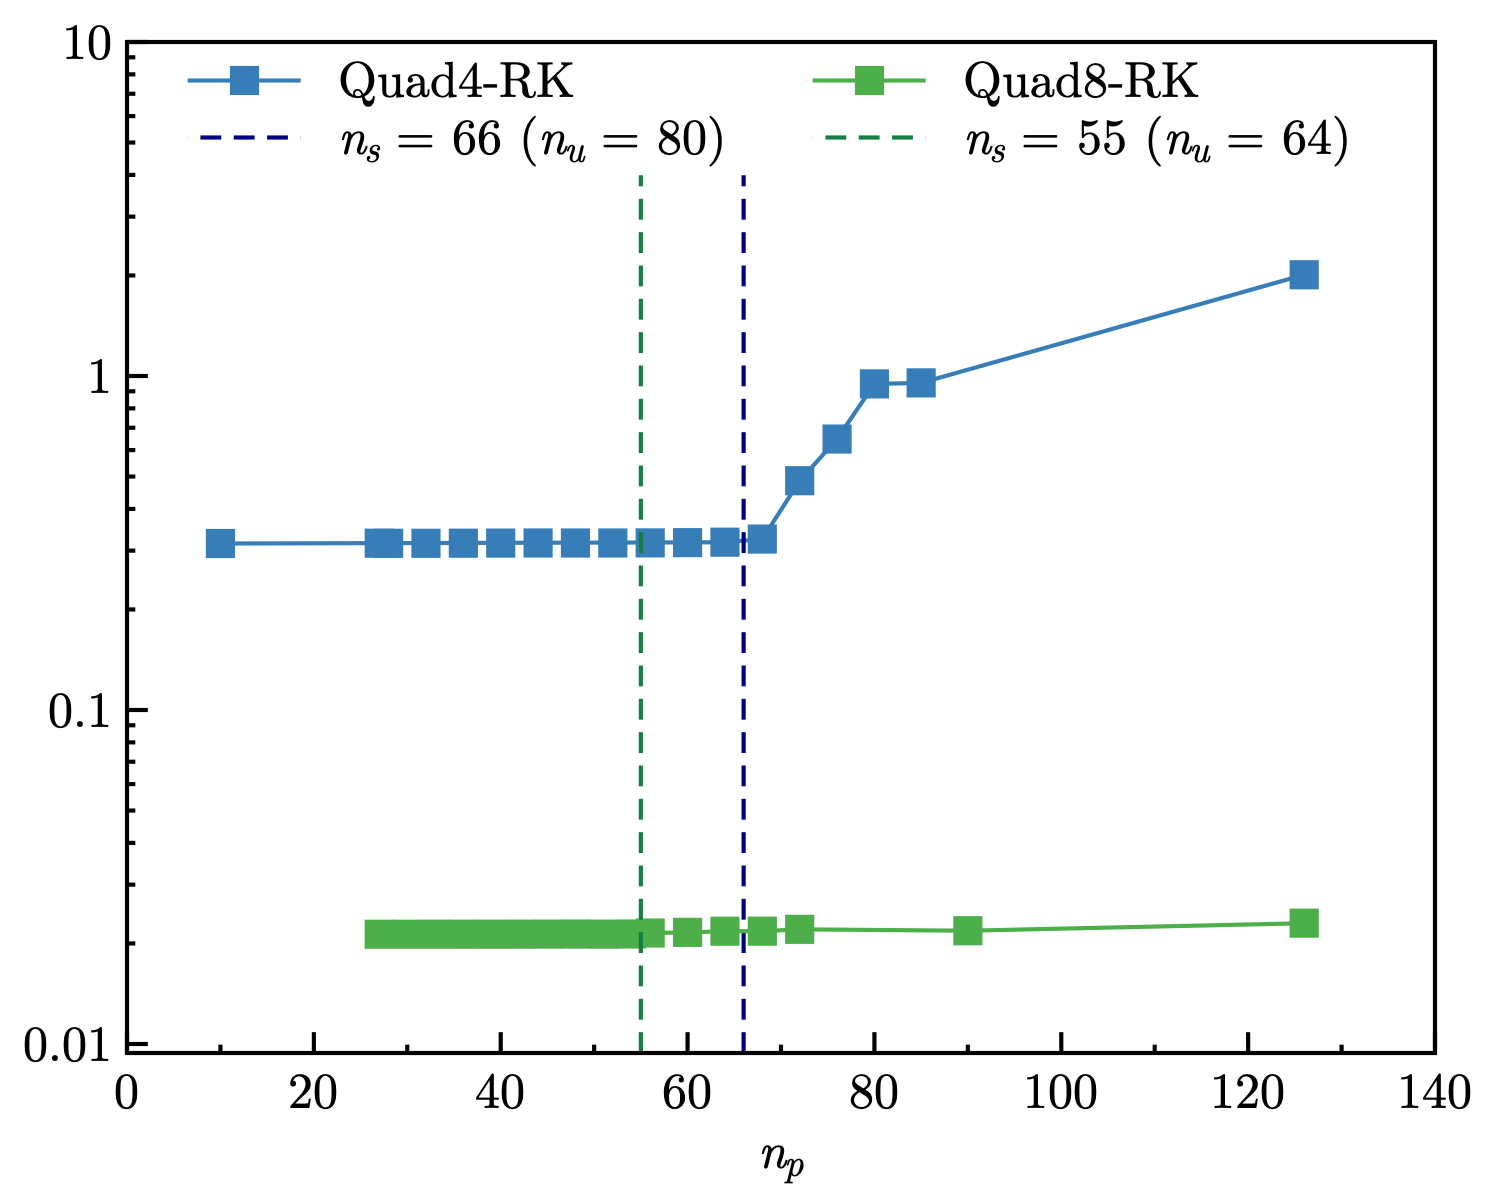
\includegraphics[width=0.48\textwidth]{png/cantilever_Hdev_4.png}}
%     & \raisebox{-0.8\height}{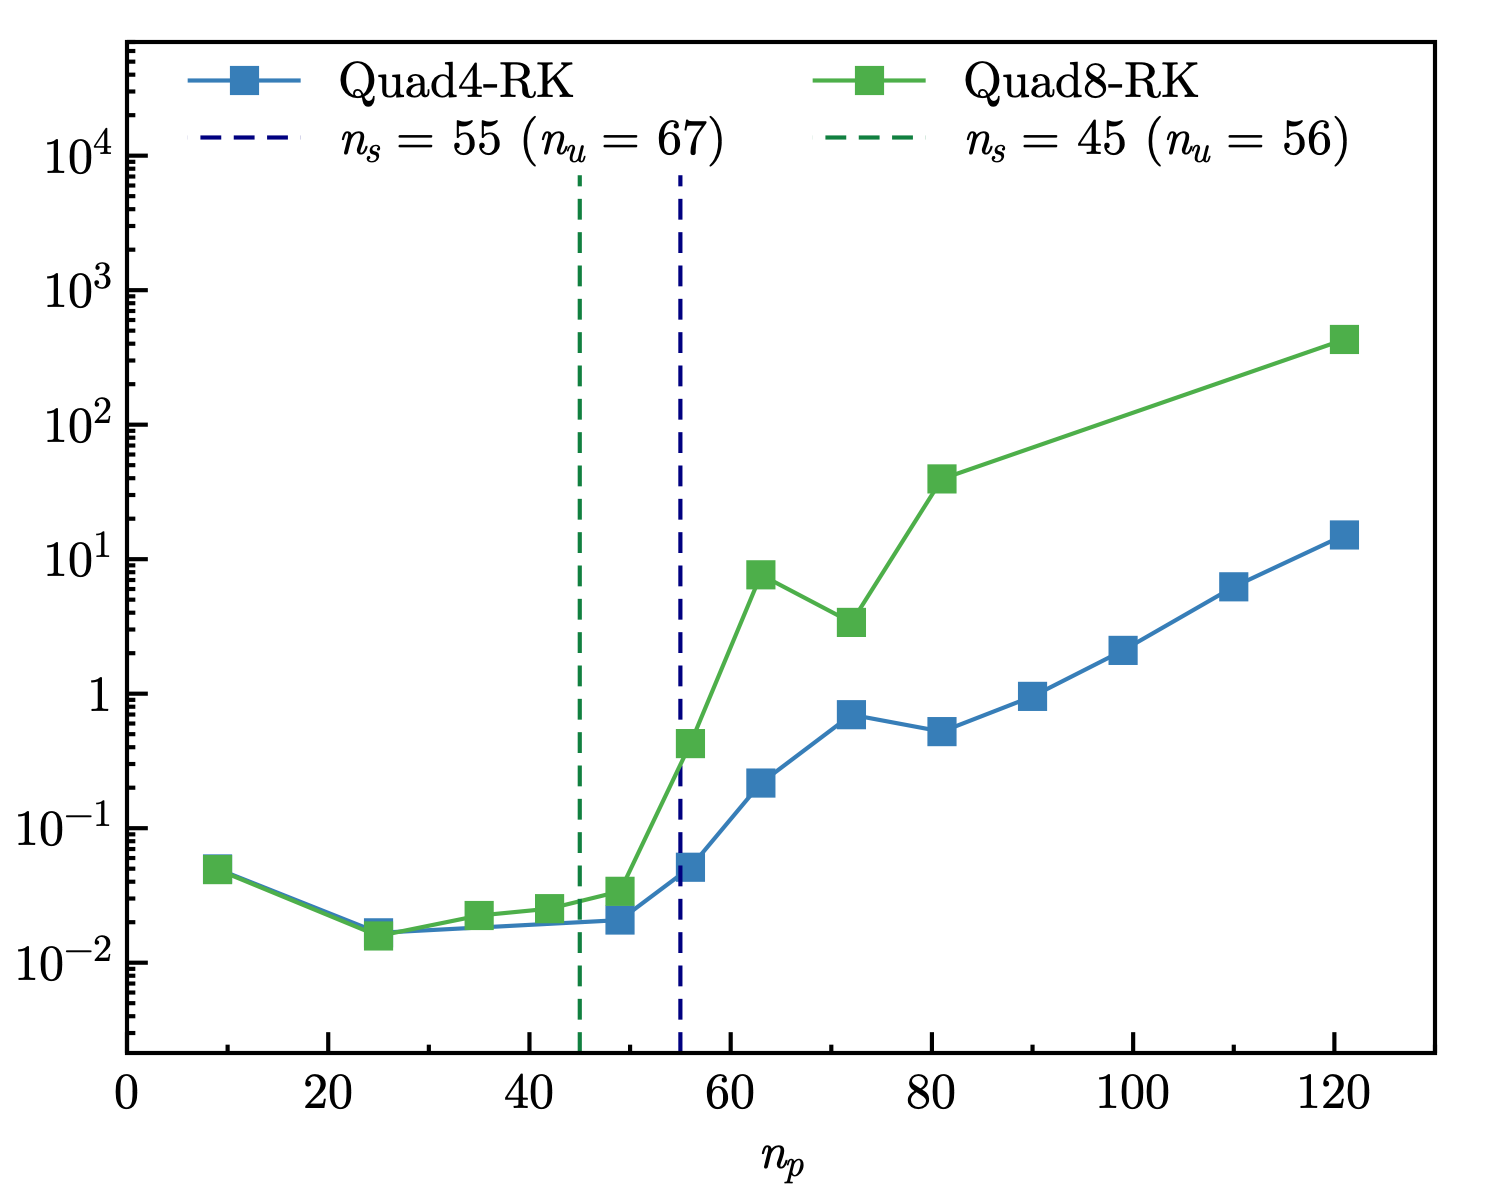
\includegraphics[width=0.48\textwidth]{png/cantilever_L2_p_4.png}}
%     \\
%       \raisebox{-0.85\height}{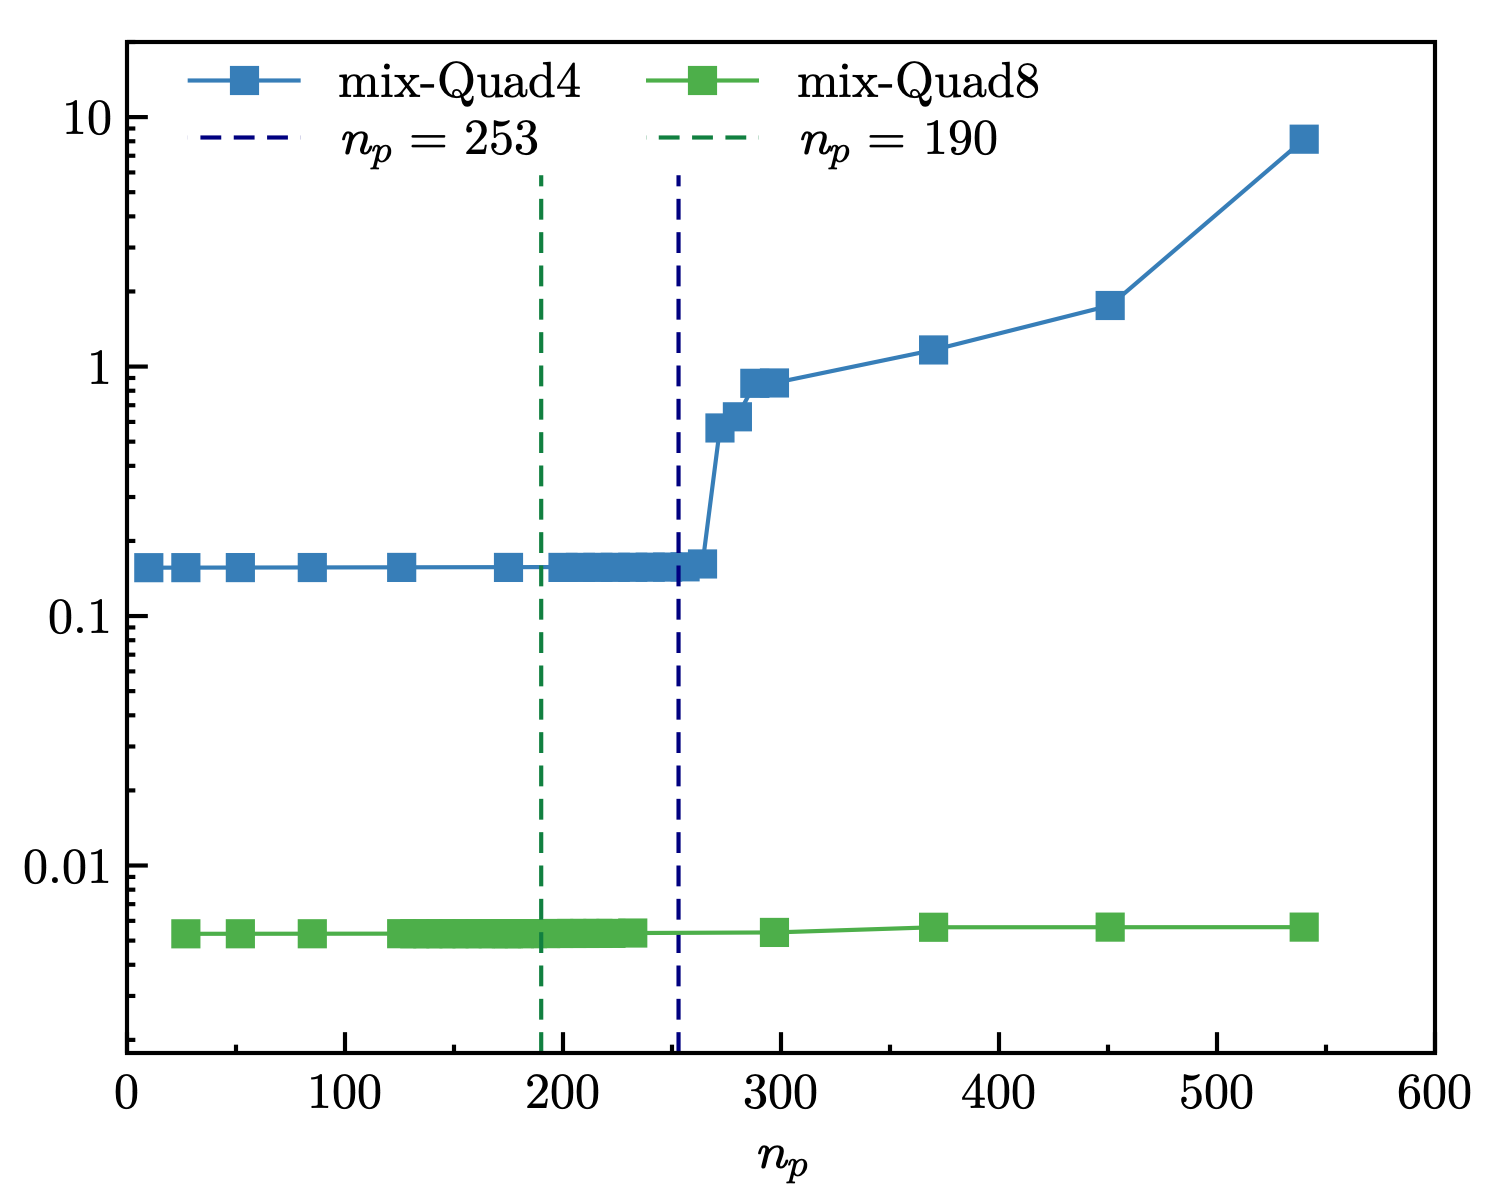
\includegraphics[width=0.48\textwidth]{png/cantilever_Hdev_8.png}}
%     & \raisebox{-0.85\height}{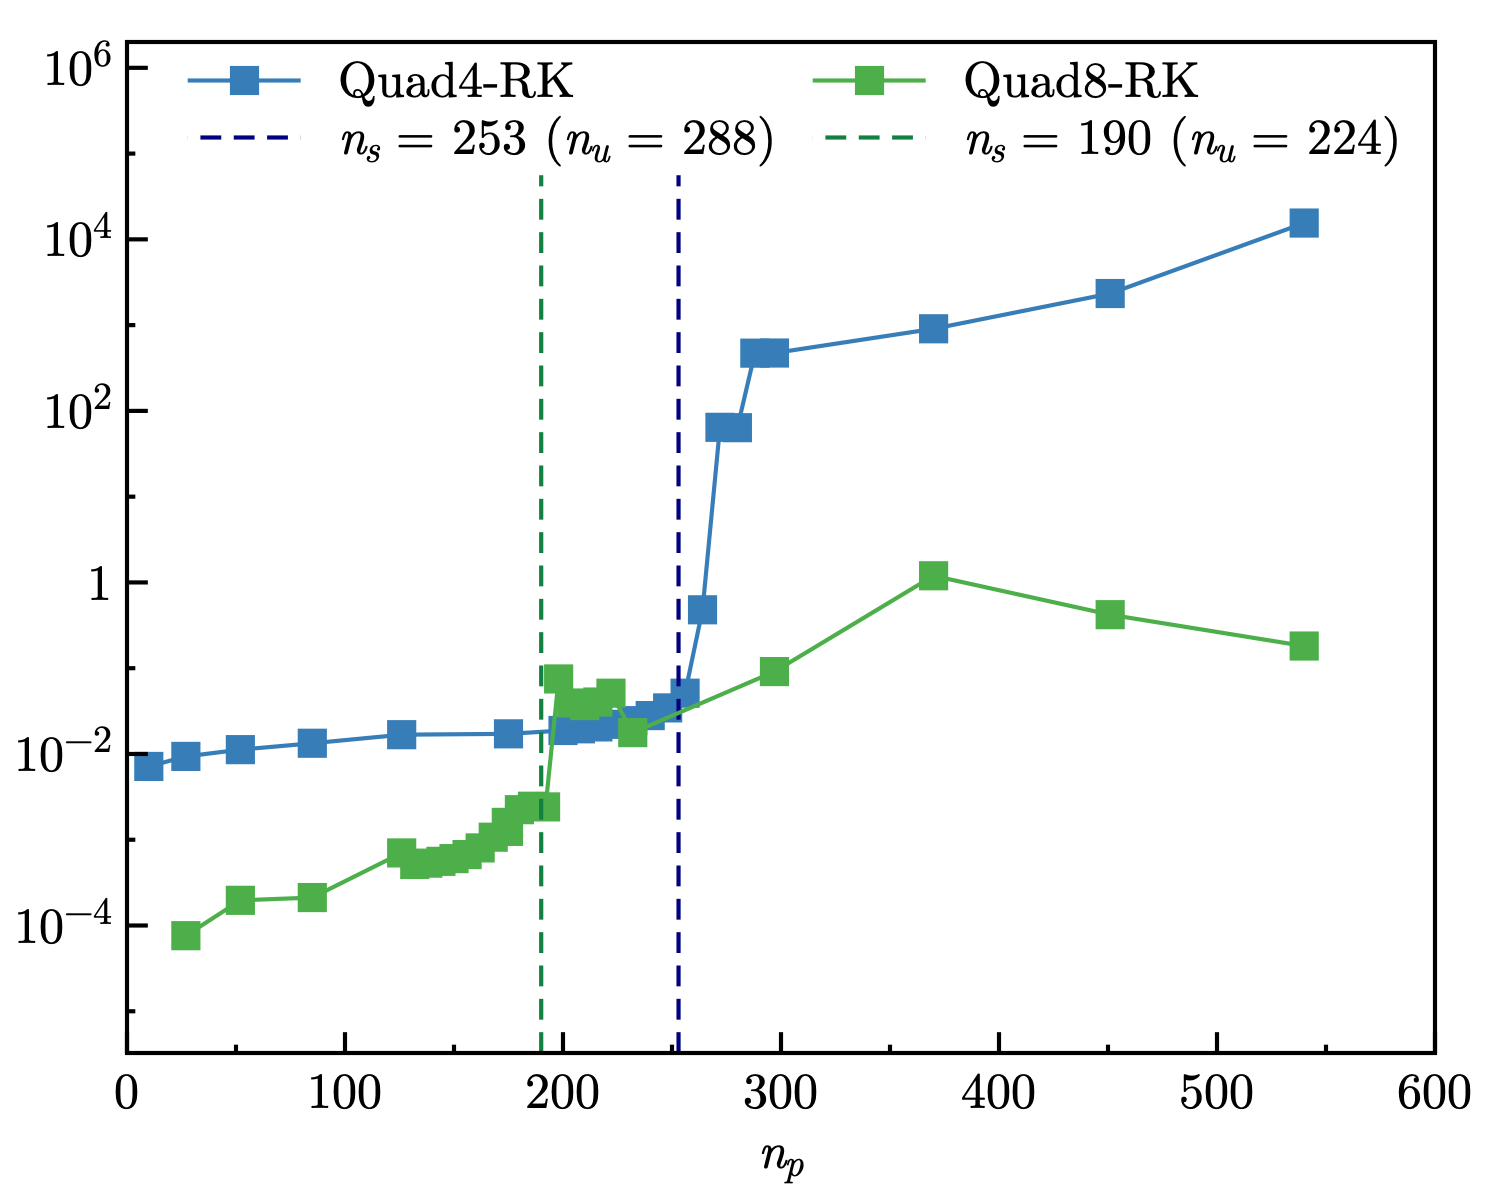
\includegraphics[width=0.48\textwidth]{png/cantilever_L2_p_8.png}}
%     \\
%       \raisebox{-0.85\height}{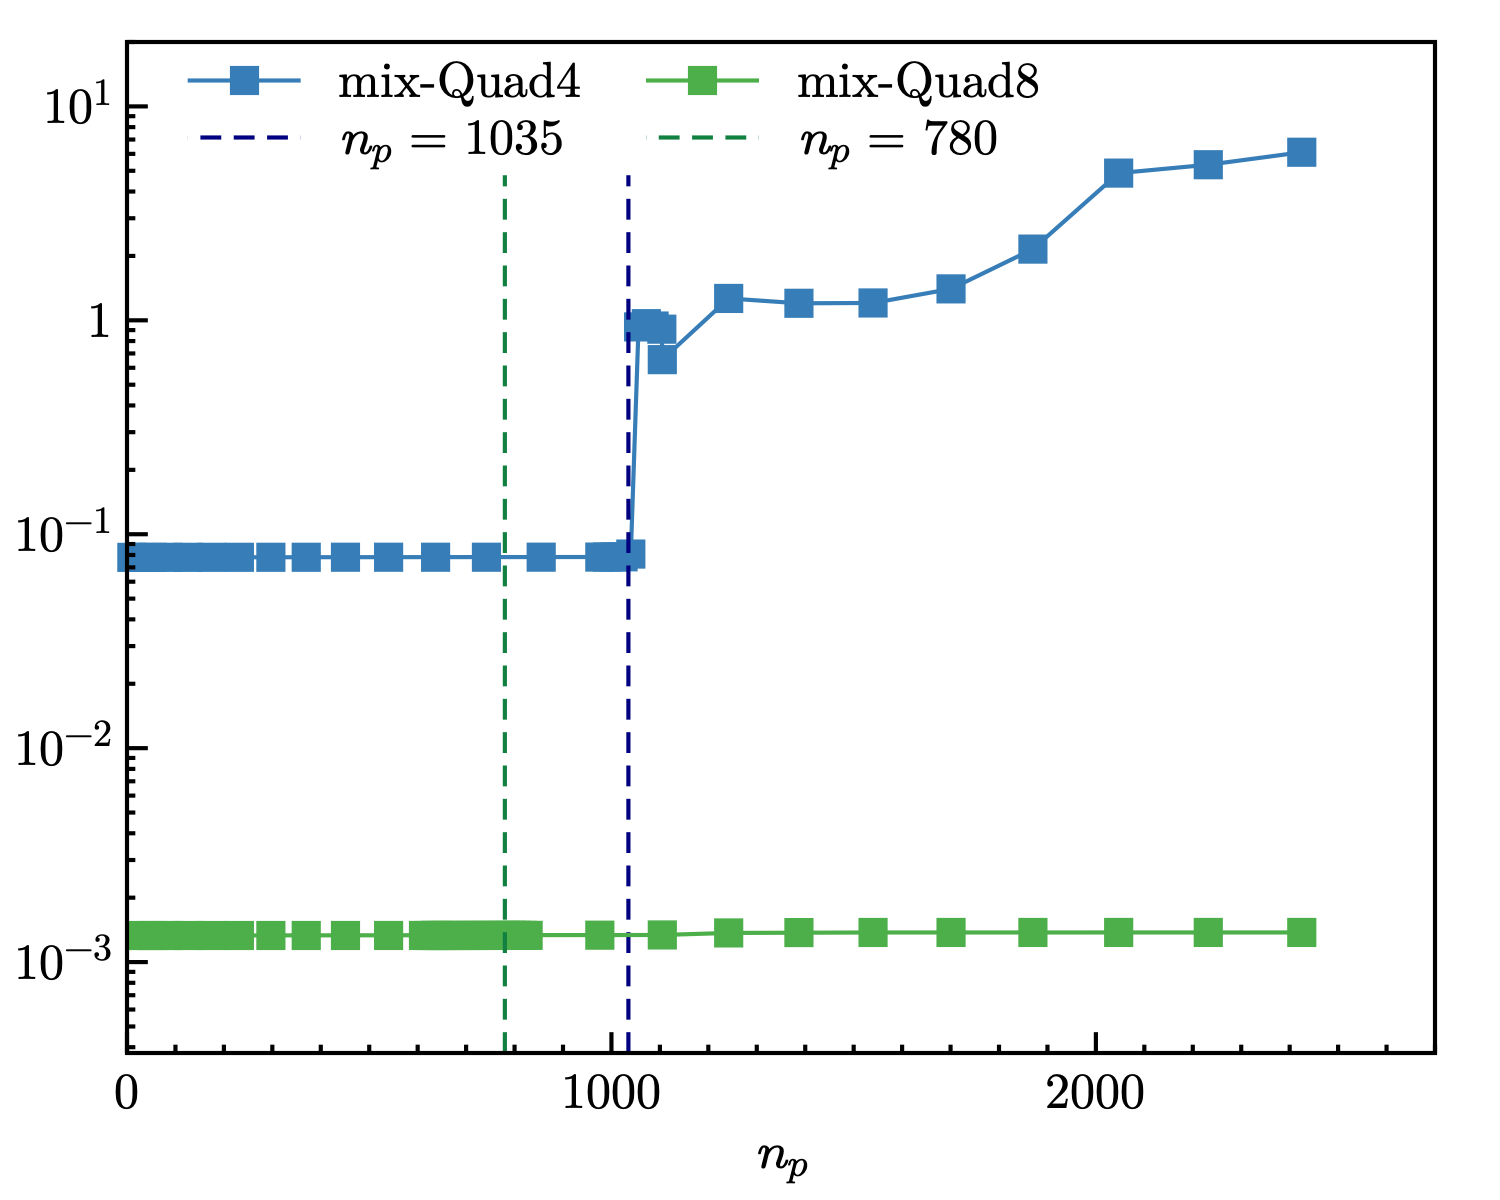
\includegraphics[width=0.48\textwidth]{png/cantilever_Hdev_16.png}}
%     & \raisebox{-0.85\height}{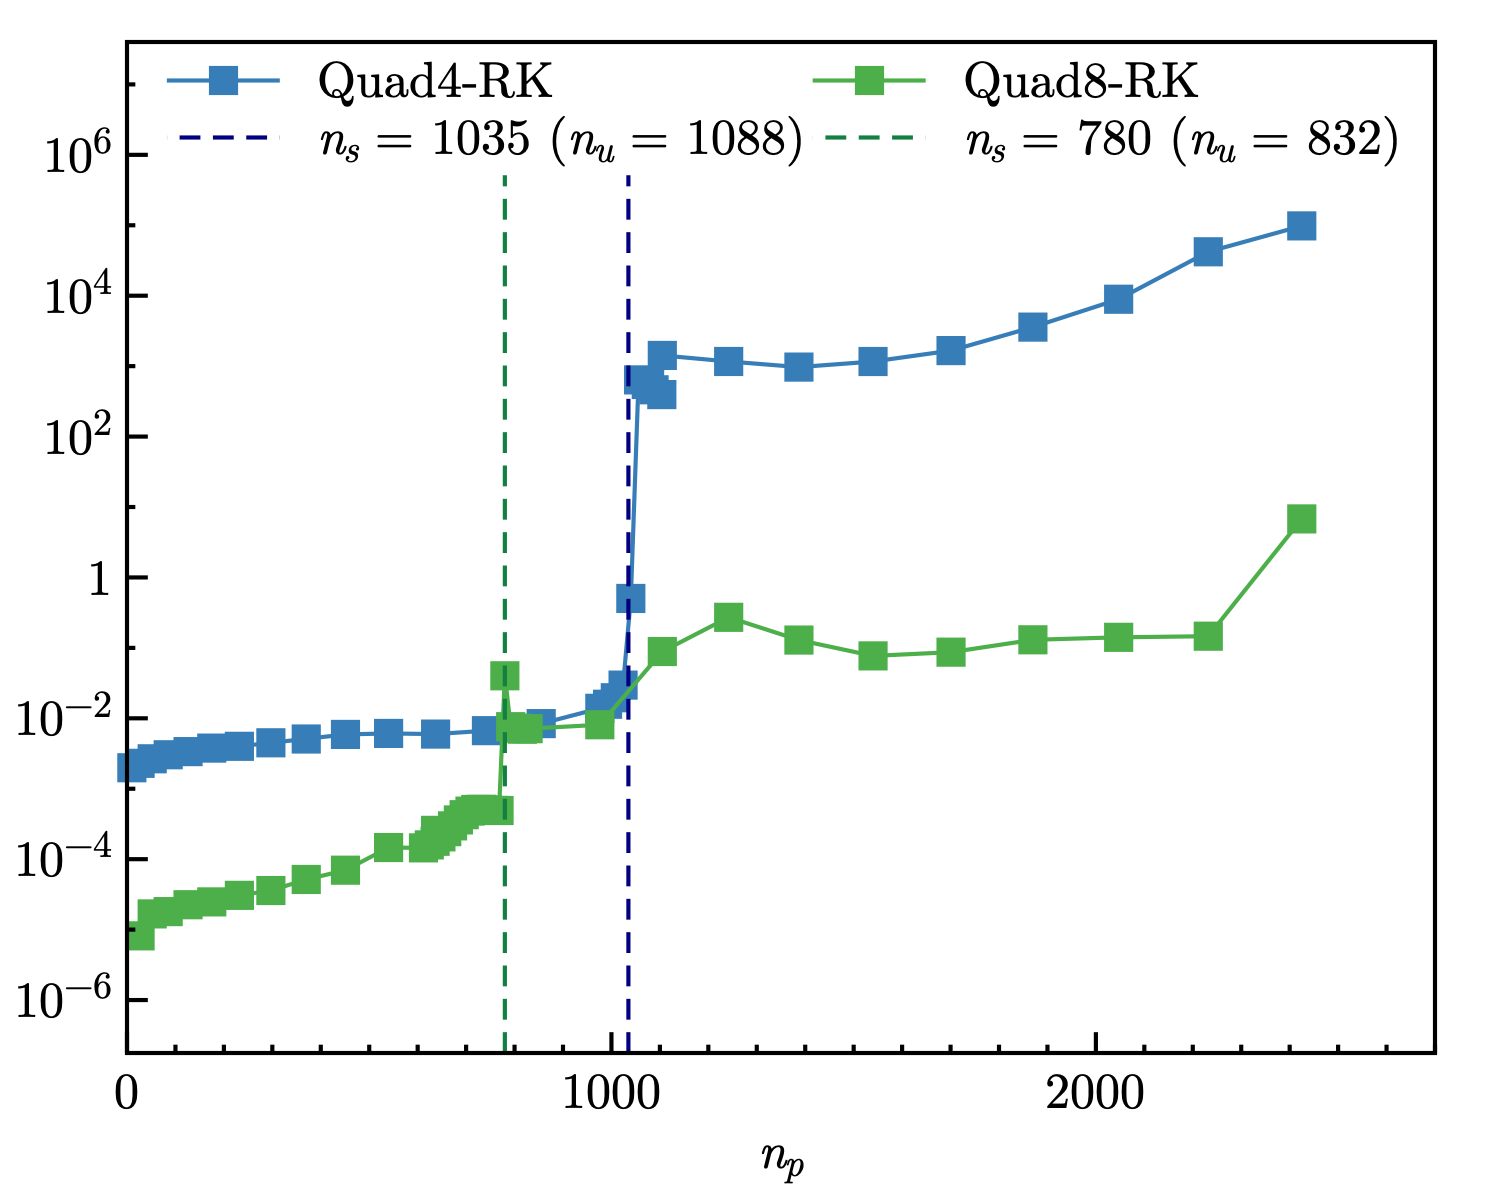
\includegraphics[width=0.48\textwidth]{png/cantilever_L2_p_16.png}}
%     \\
%       \raisebox{-0.85\height}{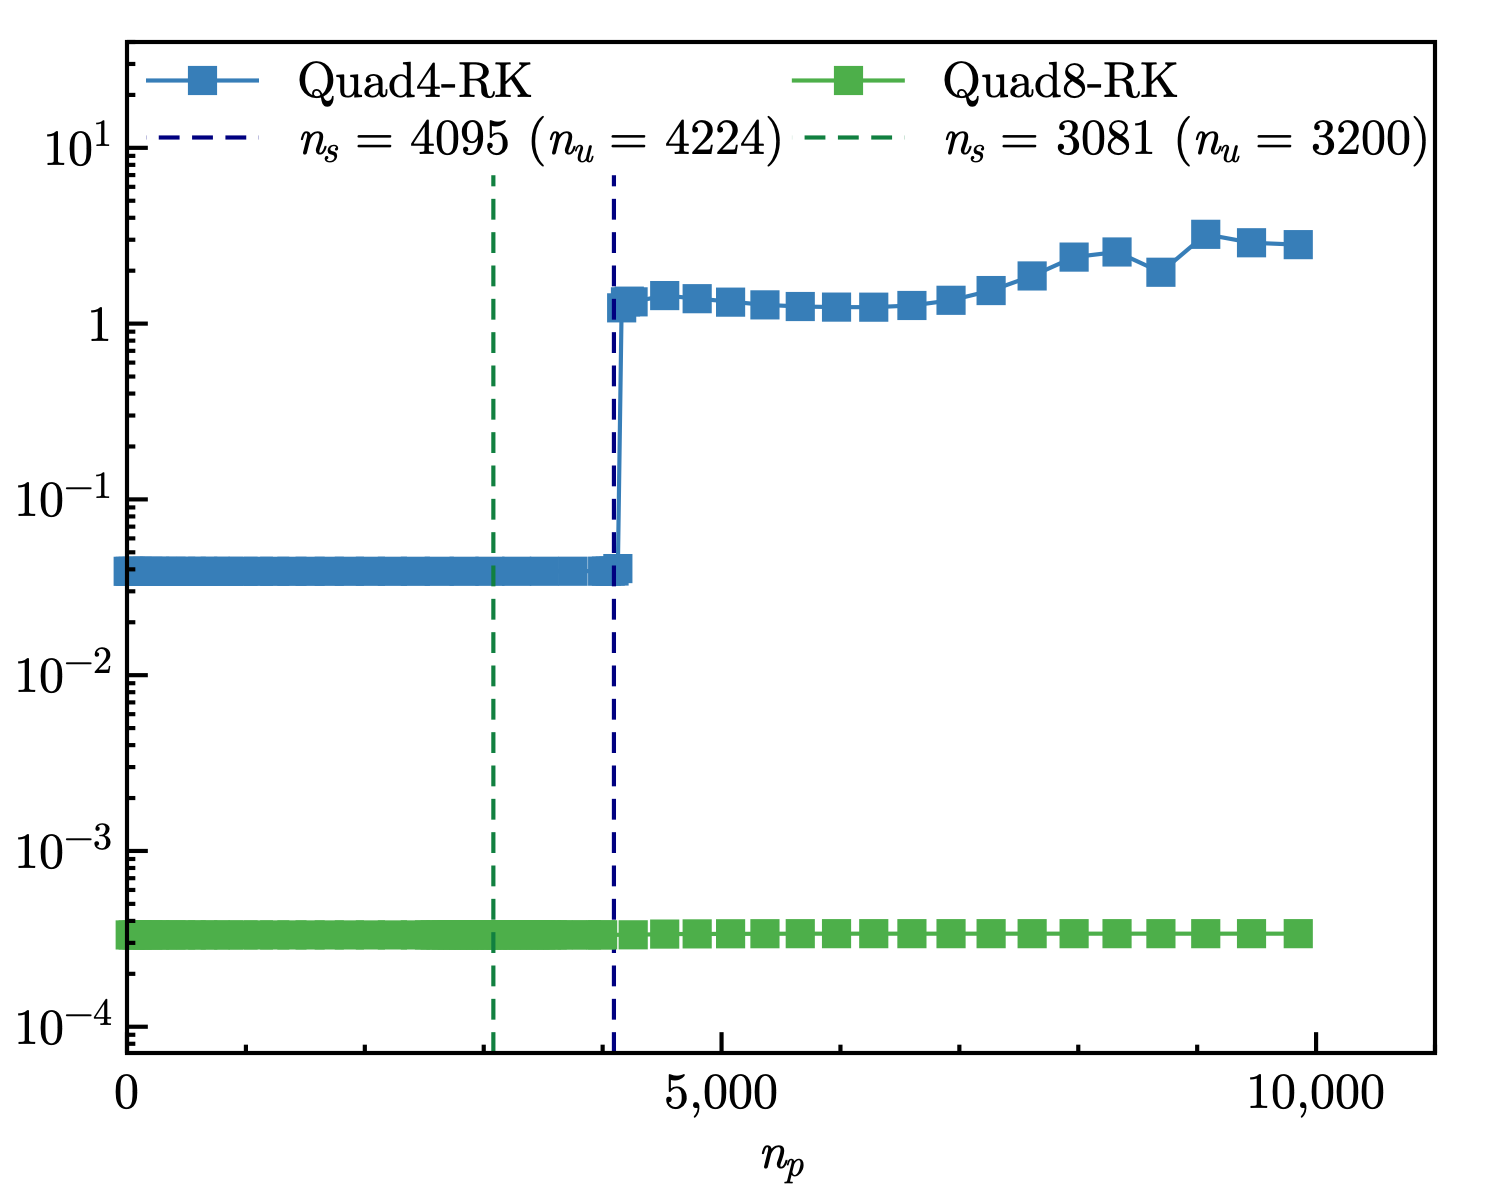
\includegraphics[width=0.48\textwidth]{png/cantilever_Hdev_32.png}}
%     & \raisebox{-0.85\height}{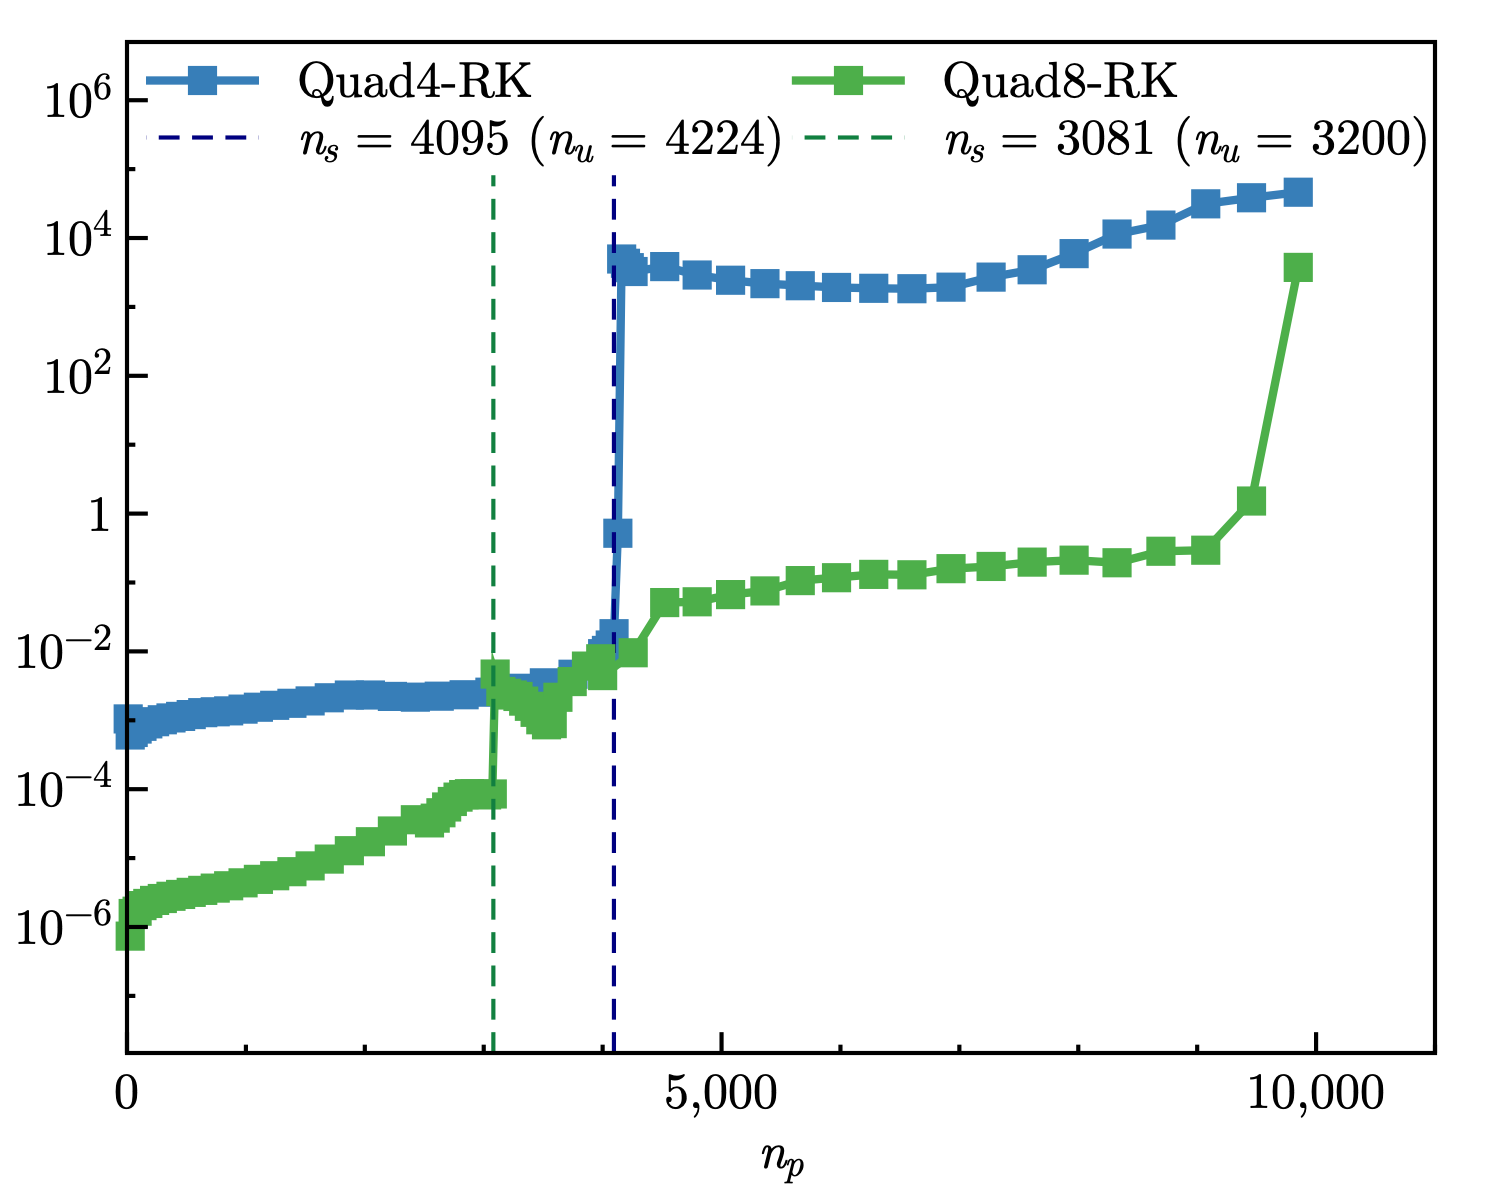
\includegraphics[width=0.48\textwidth]{png/cantilever_L2_p_32.png}}
%     \end{tabular}
% \end{subcaptiongroup}
% \caption{Strain and pressures errors v.s. $n_p$ for cantilever beam problem}\label{fg:cantilever_ns}
% \end{figure}

% \begin{figure}[H]
% \centering
% 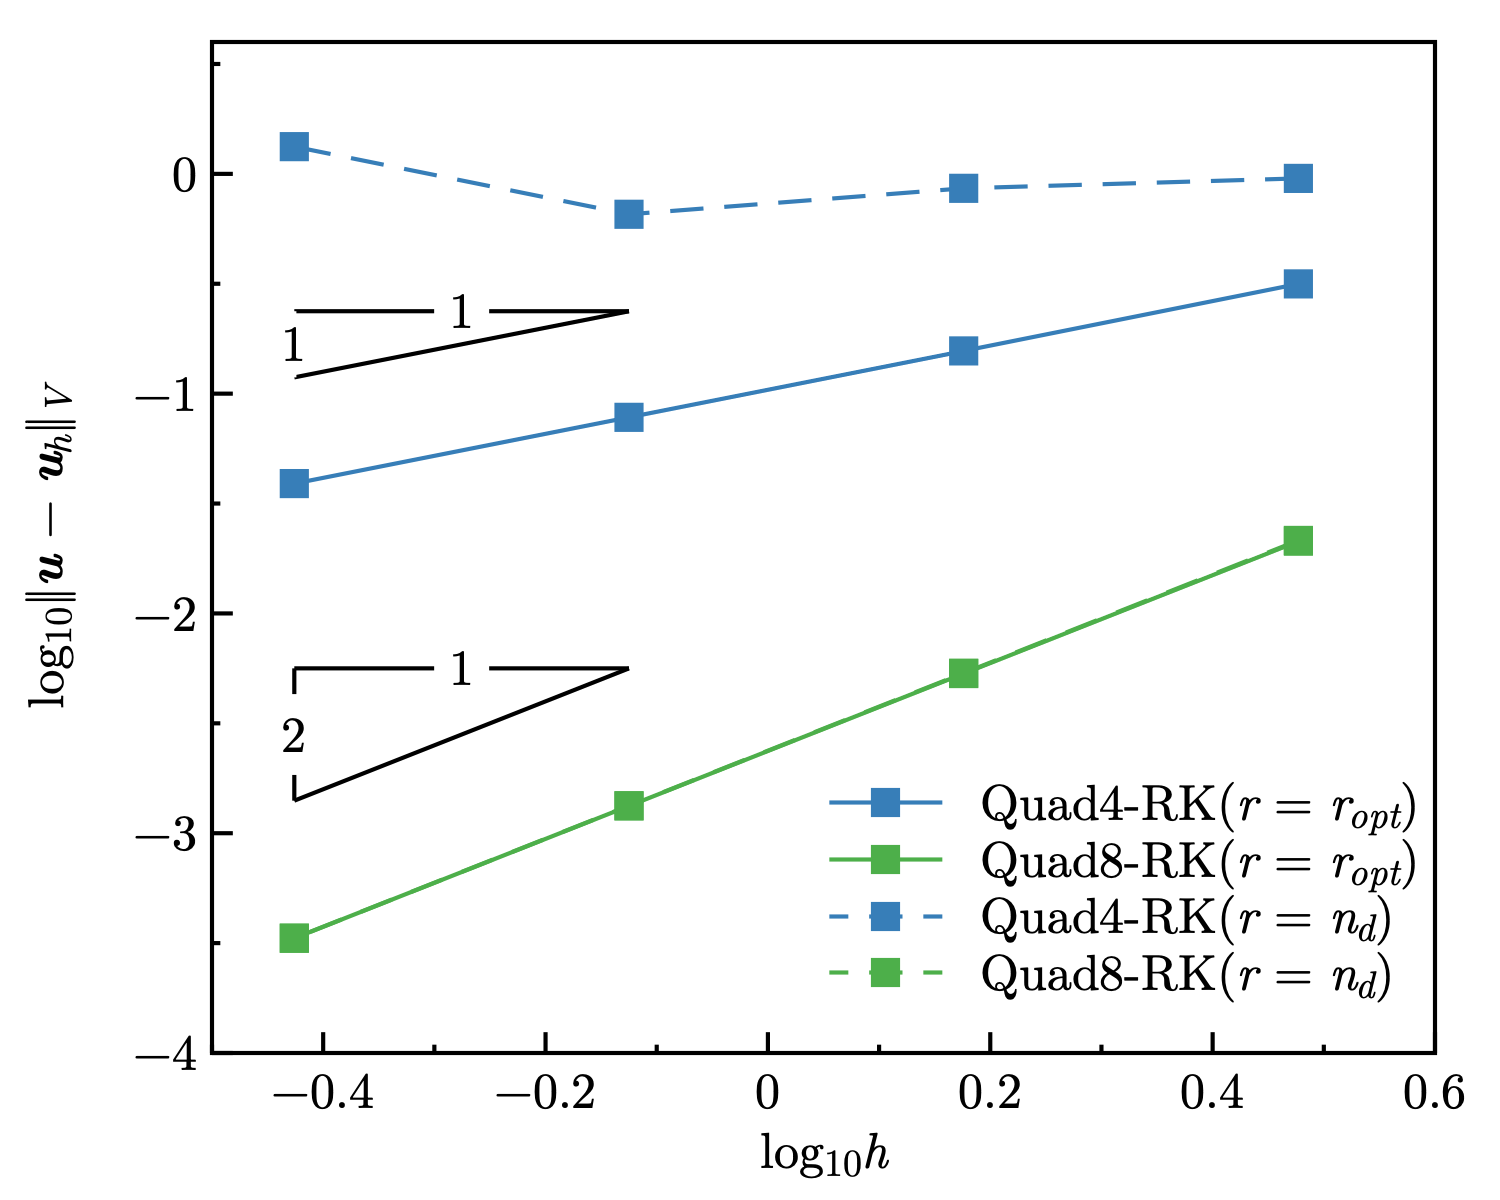
\includegraphics[width=0.49\textwidth]{png/cantilever_Hdev.png}
% 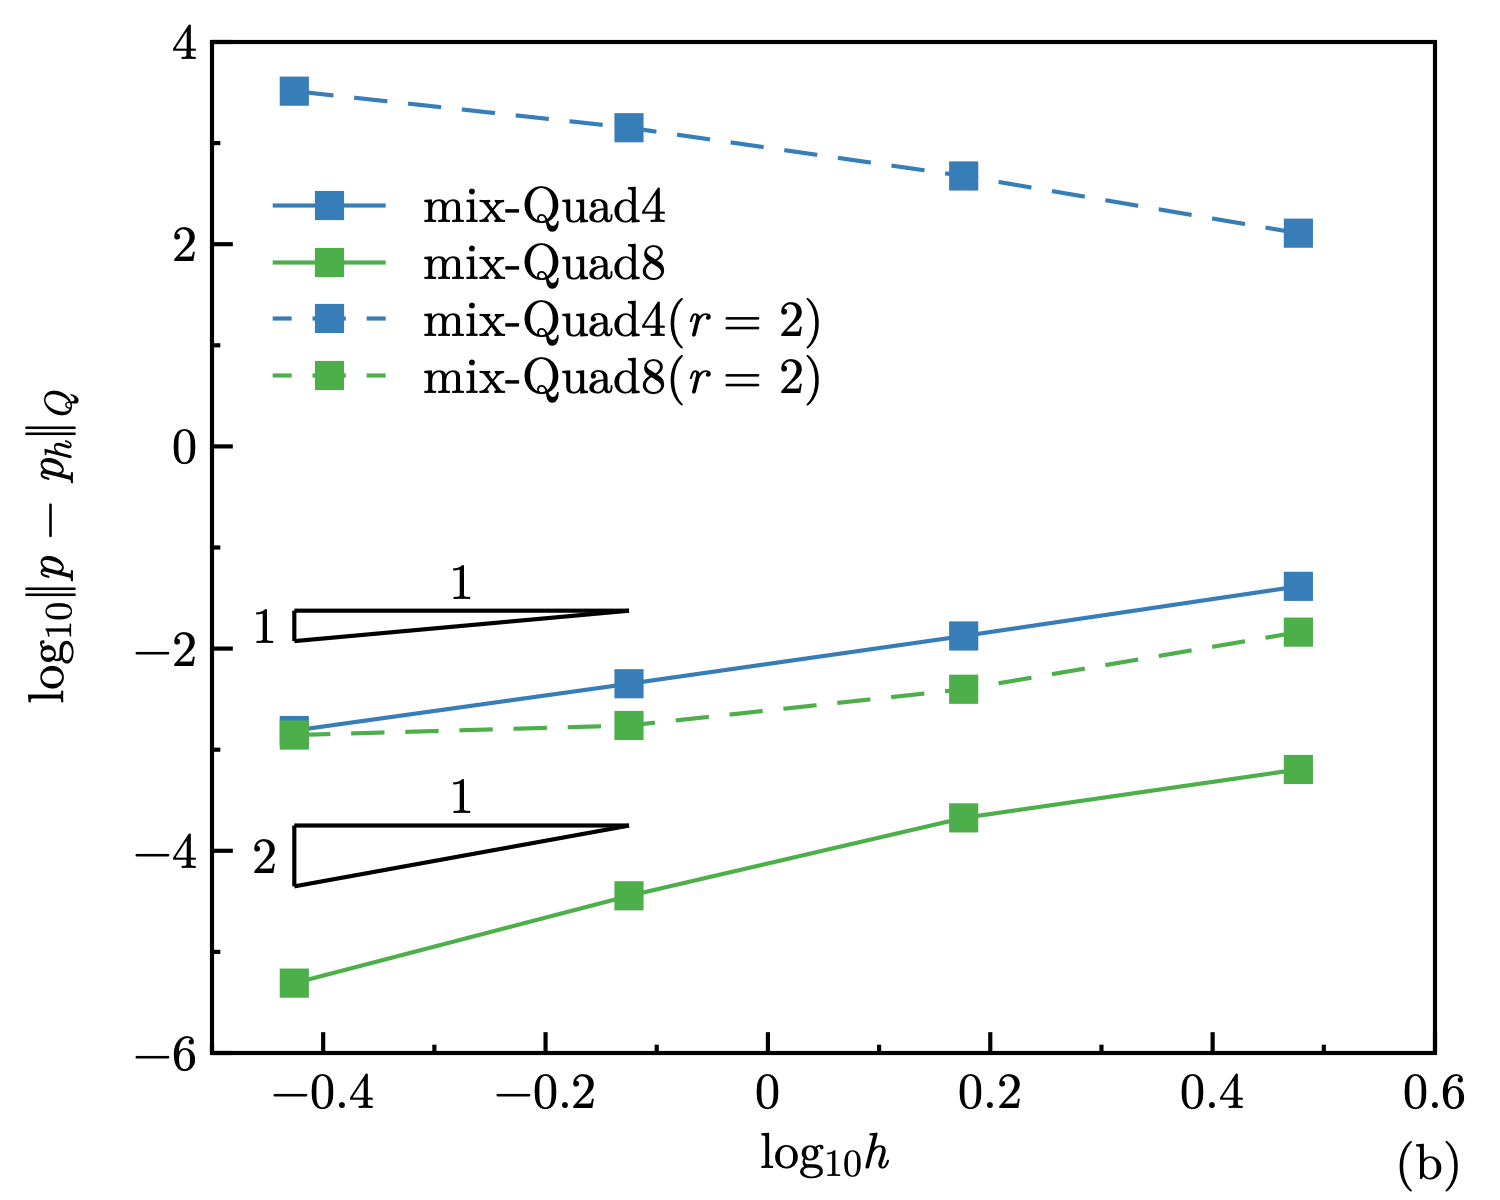
\includegraphics[width=0.49\textwidth]{png/cantilever_L2_p.png}
% \caption{Error convergence study for cantilever beam problem: (a) Strain, (b) Pressure}\label{fg:cantilever_convergence}
% \end{figure}

\subsection{Cantilever beam problem}\label{sec:cantilever}
Consider the cantilever beam problem shown in Figure \ref{fg:cantilever_model} with length $L = 48$, width $D = 12$, and the incompressible material parameters are employed with Young's modulus $E = 3\times 10^6$, Poisson's ratio $\nu = 0.5-10^{-8}$. The left hand side is fixed and the right side subject to a concentrated force $P = 1000$. All the prescribed values in the boundary conditions are evaluated by the analytical solution that is given as follows \cite{timoshenko1969theory}:
\begin{equation}
\left\{
\begin{aligned}
u_x(\boldsymbol{x}) &= - \frac{Py}{6\bar{E}I} \left( (6L - 3x)x + (2 + \bar{\nu})(y^2 - \frac{D^2}{4}) \right) \\
u_y(\boldsymbol{x}) &= \frac{P}{6\bar{E}I} \left( 3 \bar{\nu} y^2(L-x) + (4+5\bar{\nu}) \frac{D^2x}{4} + (3L-x)x^2 \right)
\end{aligned}
\right.
\end{equation}
where $I$ is the beam's moment of inertia, $\bar{E}$ and $\bar{\nu}$ are the material parameters for plane strain hypothesis, they can be expressed by:
\begin{equation}
I = \frac{D^3}{12}, \quad \bar{E} = \frac{E}{1-\nu^2}, \quad \bar{\nu} = \frac{\nu}{1-\nu}
\end{equation}
And correspondingly, the stress components are evaluated by
\begin{equation}
\left\{
\begin{aligned}
\sigma_{xx} &= - \frac{P(L-x)y}{I} \\
\sigma_{yy} &= 0 \\
\sigma_{xy} &= \frac{P}{2I}(\frac{D^2}{4}-y^2)
\end{aligned}
\right.
\end{equation}

\begin{figure}[H]
\centering
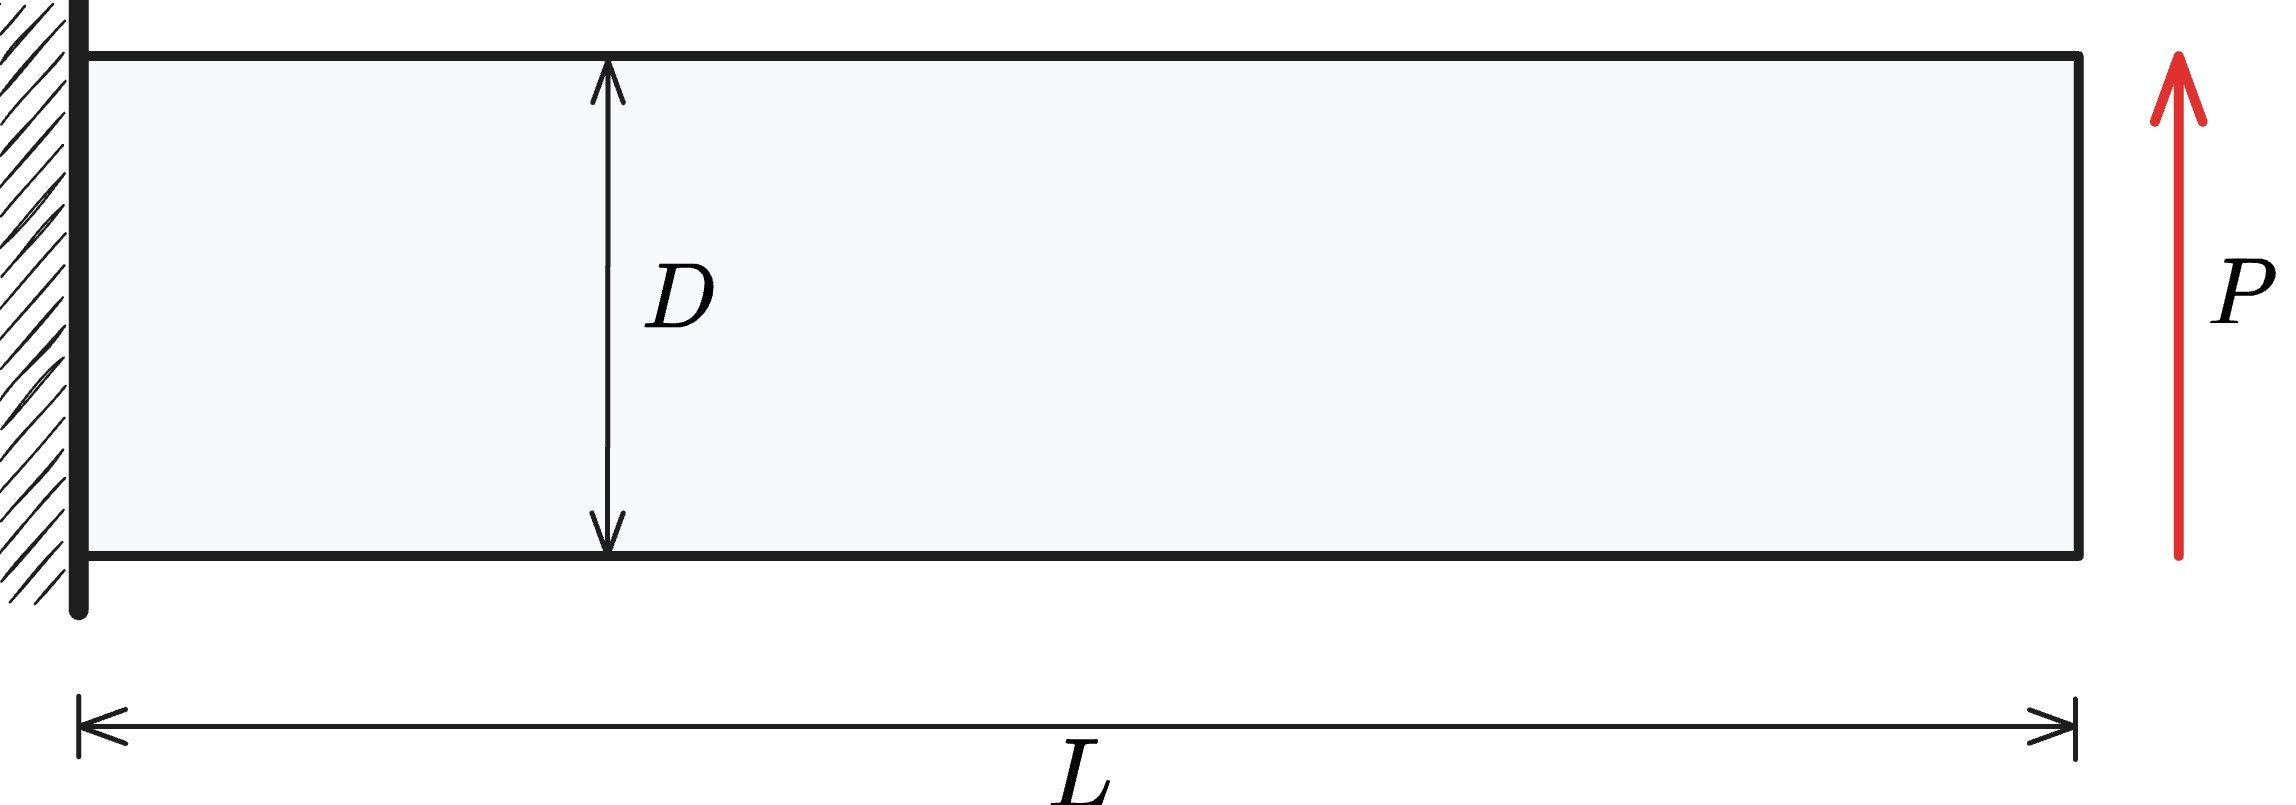
\includegraphics[width=0.7\textwidth]{png/cantilever_model.png}
\caption{Illustration of cantilever beam problem}\label{fg:cantilever_model}
\end{figure}

In this problem, the Quad4 element with $16\times 4$, $32\times 8$, $64\times 16$, $128\times 32$ grids, and Quad8 element with $8\times 2$, $16\times 4$, $32\times 8$, $64\times 16$ grids are employed for displacement discretization. The pressure is discretized by linear and quadratic meshfree approximations with 1.5 and 2.5 characterized support sizes respectively. The strain and pressure errors with respect to pressure nodes $n_p$ are displayed in Figure \ref{fg:cantilever_ns}, where the vertical dashed lines stand for the stabilized number $n_s$. The figure implies that the Quad8 shows better performance than Quad4, since the Quad8's displacement results are stable no matter the constraint ratio is in the optimal range or not. And the Quad4's displacement errors increase as soon as $n_p > n_s$. However, both Quad4's and Quad8's pressure errors immediately increase while their constraint ratios are out of the optimal range, and Quad8 still has better results than Quad4. Figure \ref{fg:cantilever_convergence} shows the strain and pressure error convergence comparisons for this cantilever beam problem, in which, except Quad8--RK($r=2$) for strain error, all formulations with the traditional constraint ratio of $r=2$ cannot ensure the optimal error convergence rates. The proposed mixed formulations with $r=r_{opt}$ can maintain the optimal error convergence ratio and show better accuracy.

\begin{figure}[H]
\centering
\begin{subcaptiongroup}
\begin{tabular}{c@{\hspace{0pt}}c}
$\Vert \boldsymbol{u} - \boldsymbol{u}_h \Vert_V$ & $\Vert p - p_h \Vert_Q$ \\
\raisebox{-0.8\height}{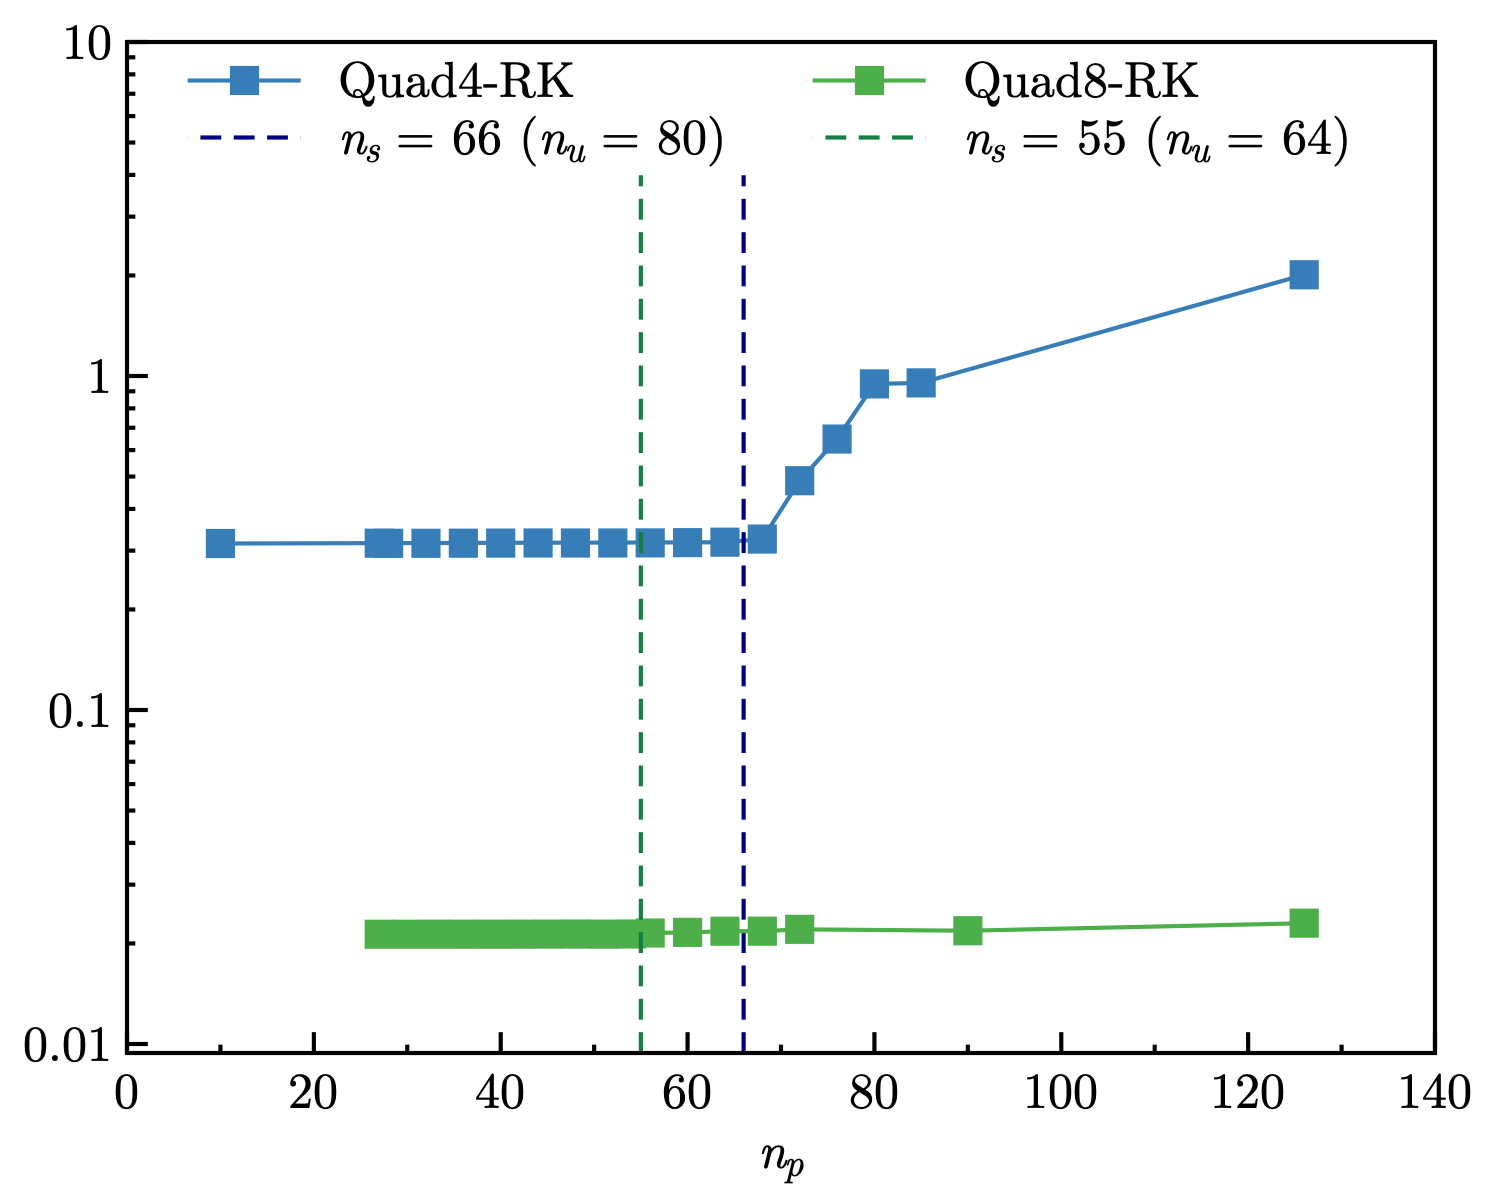
\includegraphics[width=0.48\textwidth]{png/cantilever_Hdev_4.png}}
& \raisebox{-0.8\height}{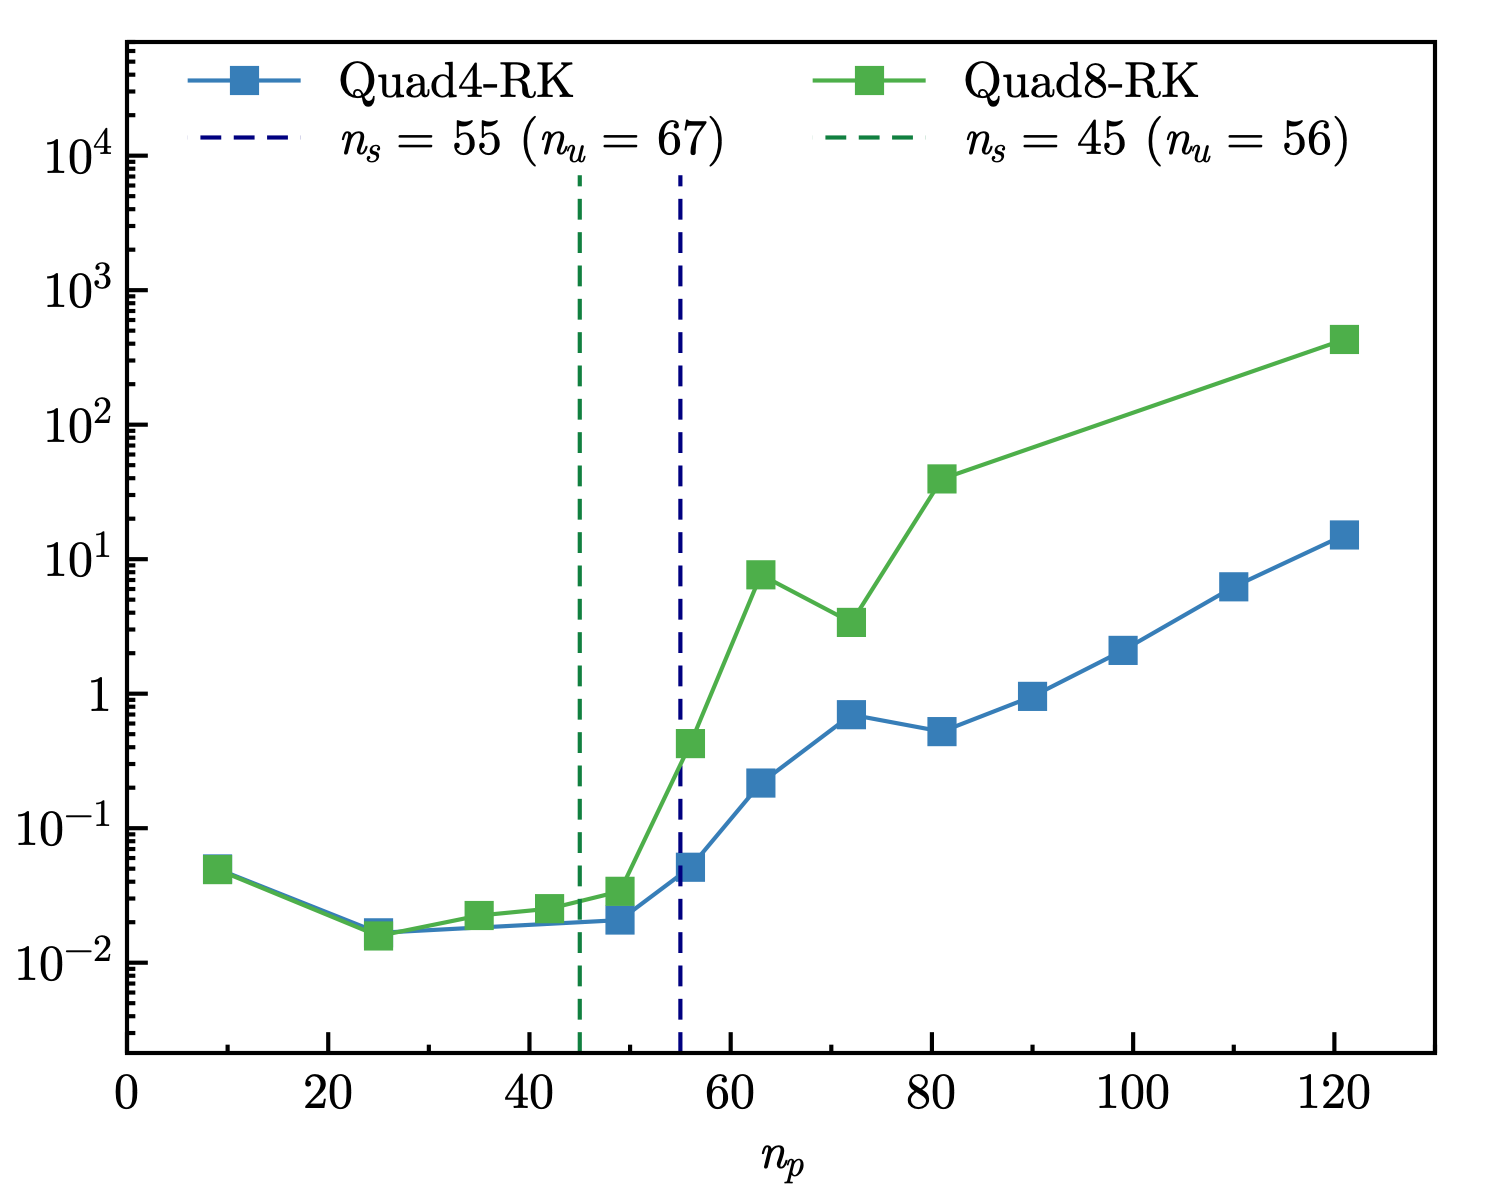
\includegraphics[width=0.48\textwidth]{png/cantilever_L2_p_4.png}} \\
\raisebox{-0.85\height}{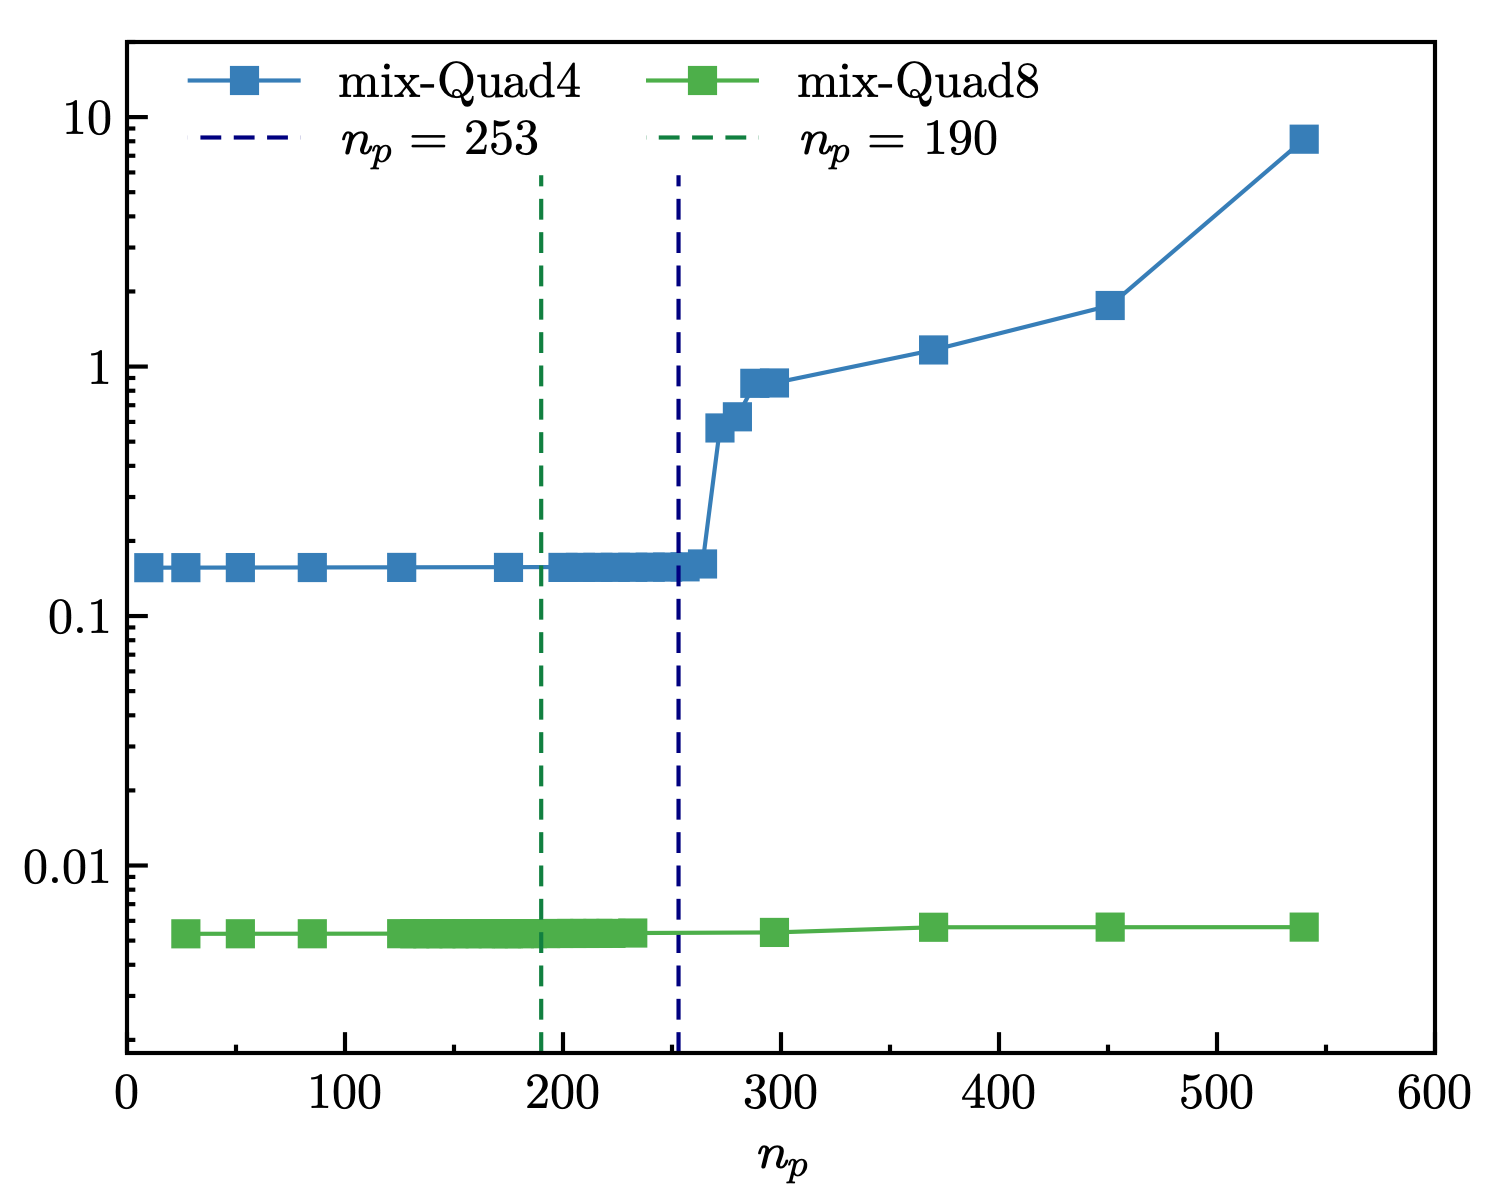
\includegraphics[width=0.48\textwidth]{png/cantilever_Hdev_8.png}}
& \raisebox{-0.85\height}{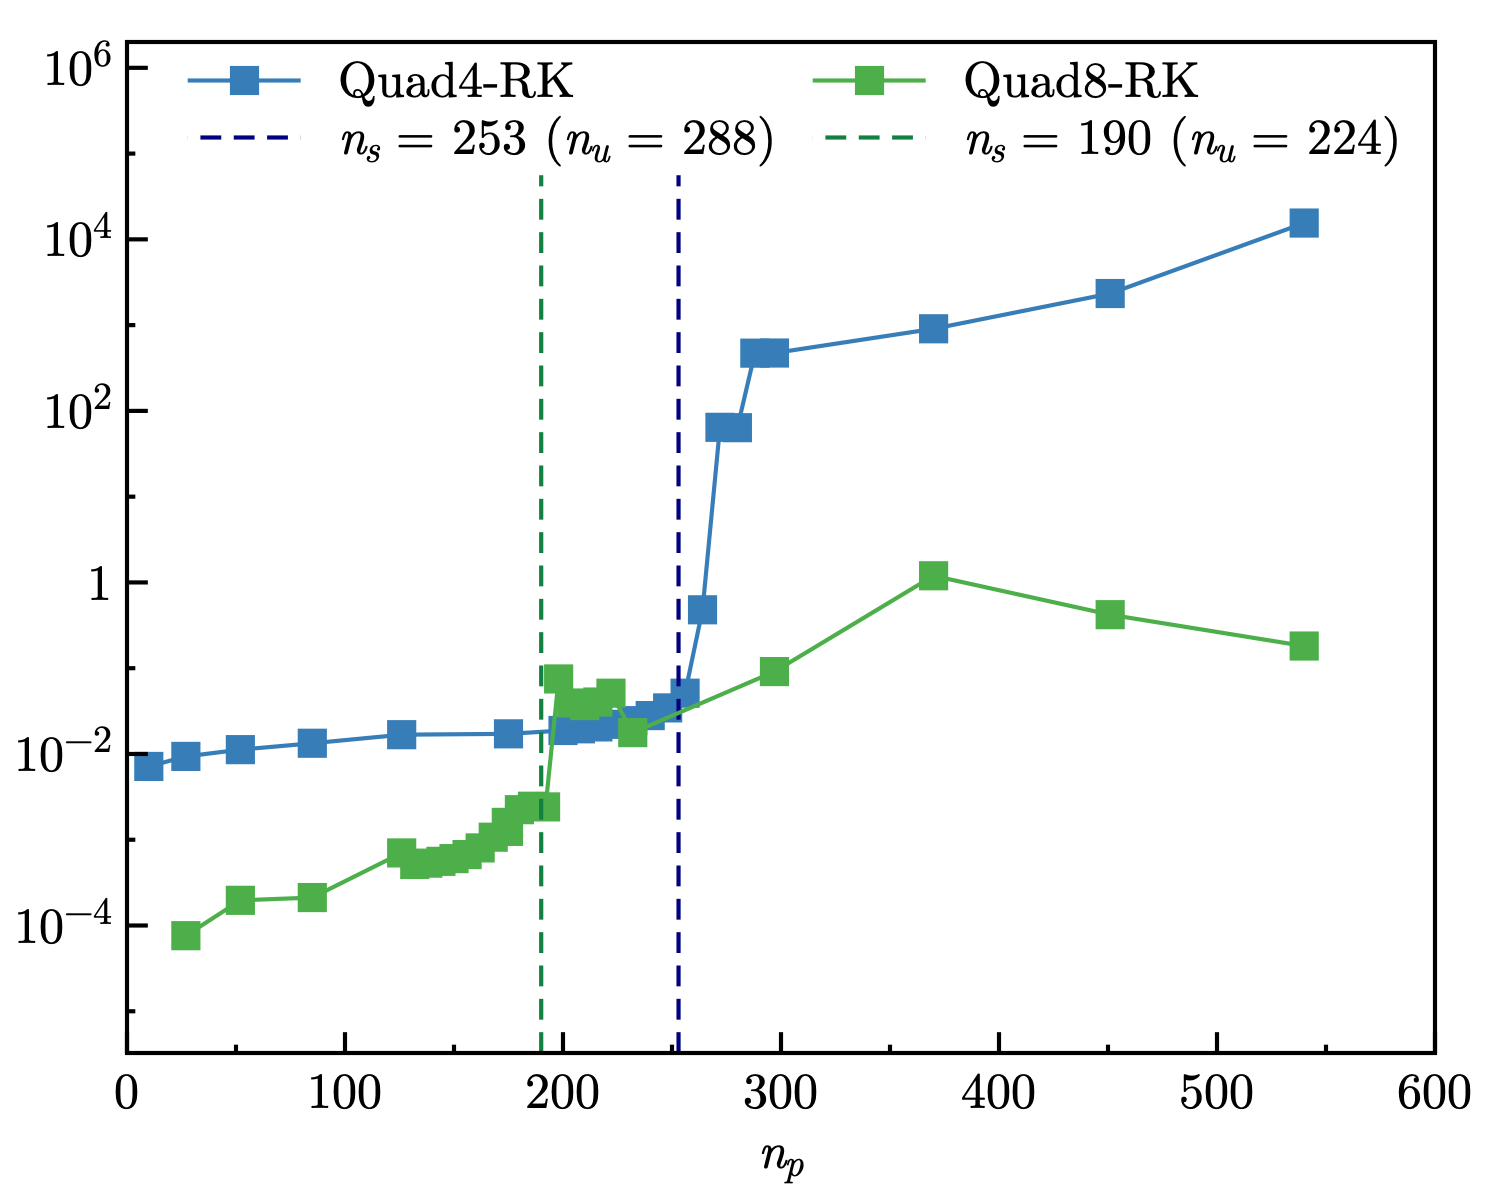
\includegraphics[width=0.48\textwidth]{png/cantilever_L2_p_8.png}} \\
\raisebox{-0.85\height}{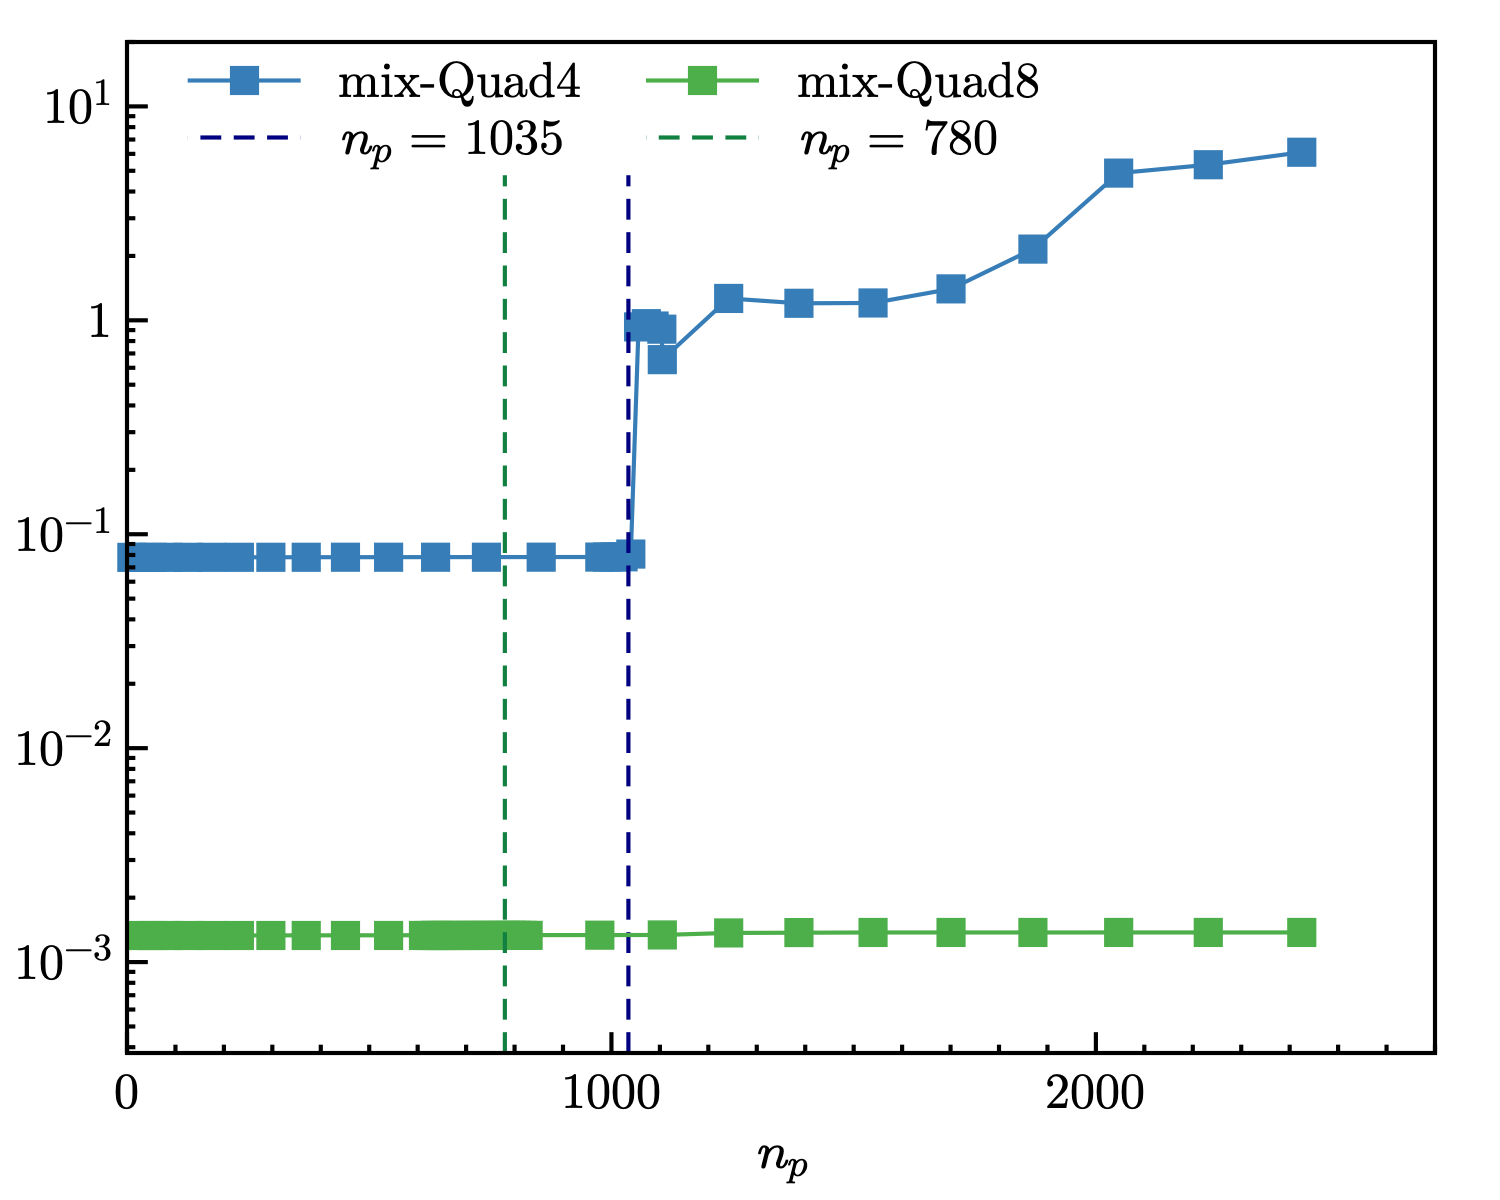
\includegraphics[width=0.48\textwidth]{png/cantilever_Hdev_16.png}}
& \raisebox{-0.85\height}{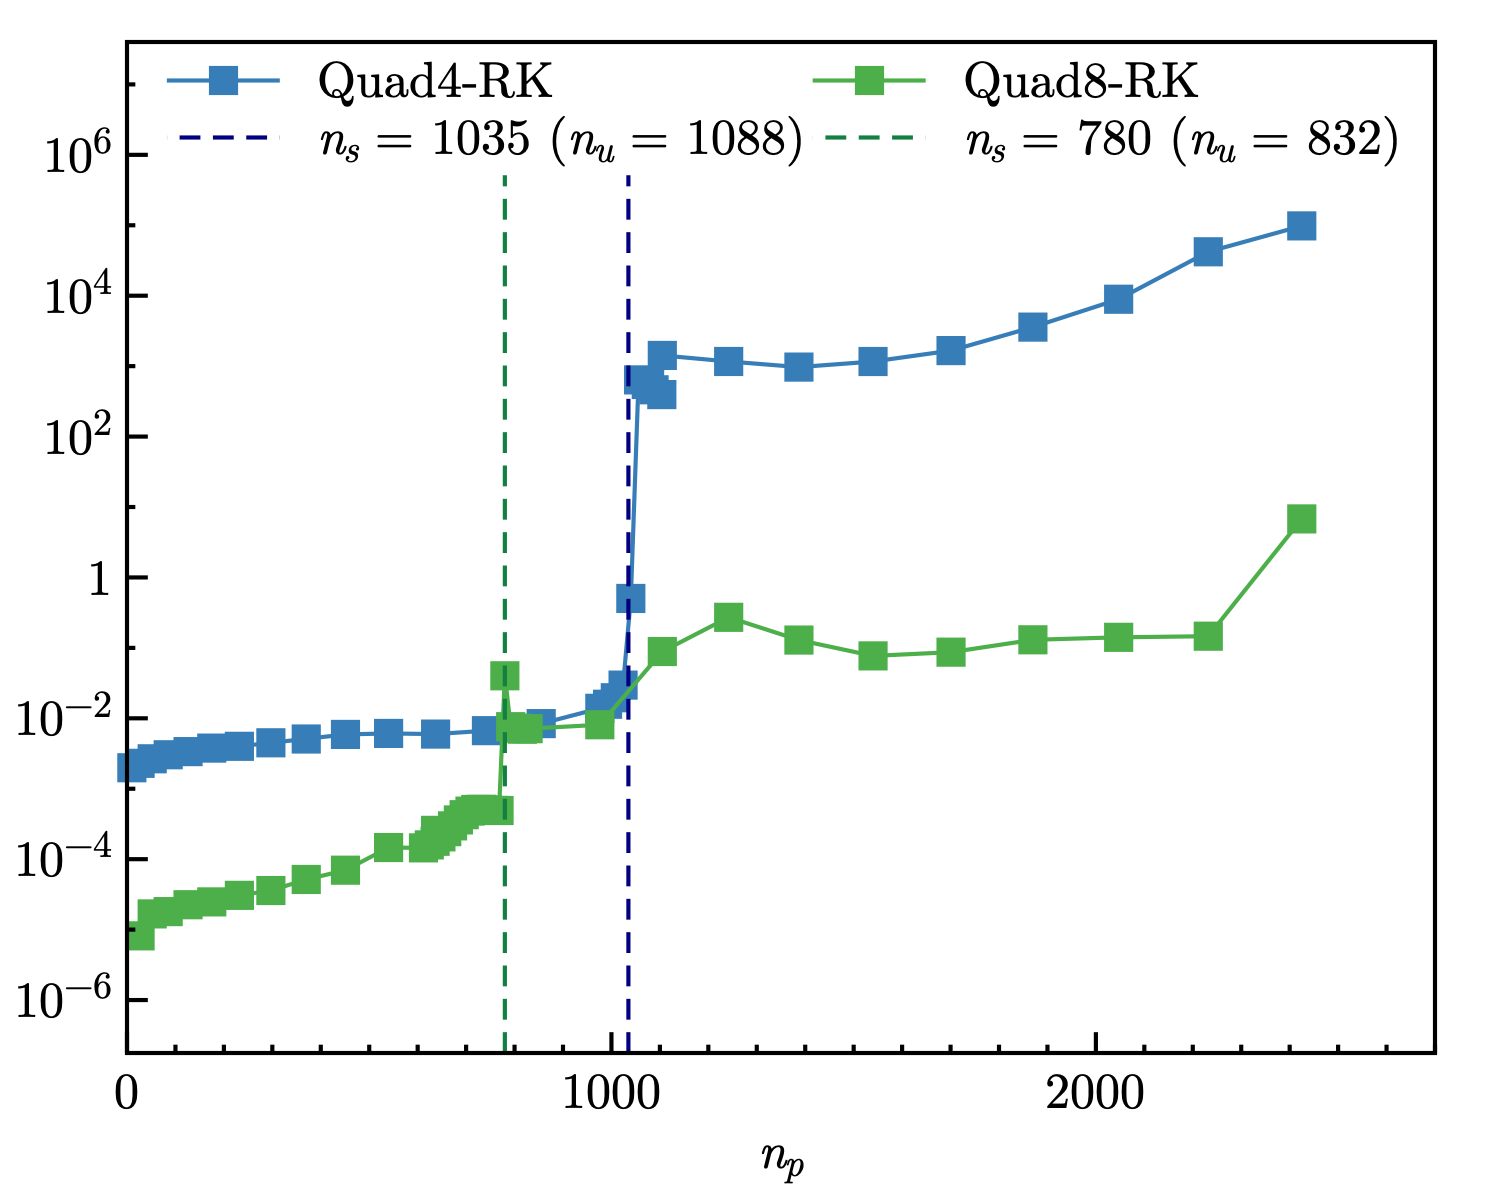
\includegraphics[width=0.48\textwidth]{png/cantilever_L2_p_16.png}} \\
\raisebox{-0.85\height}{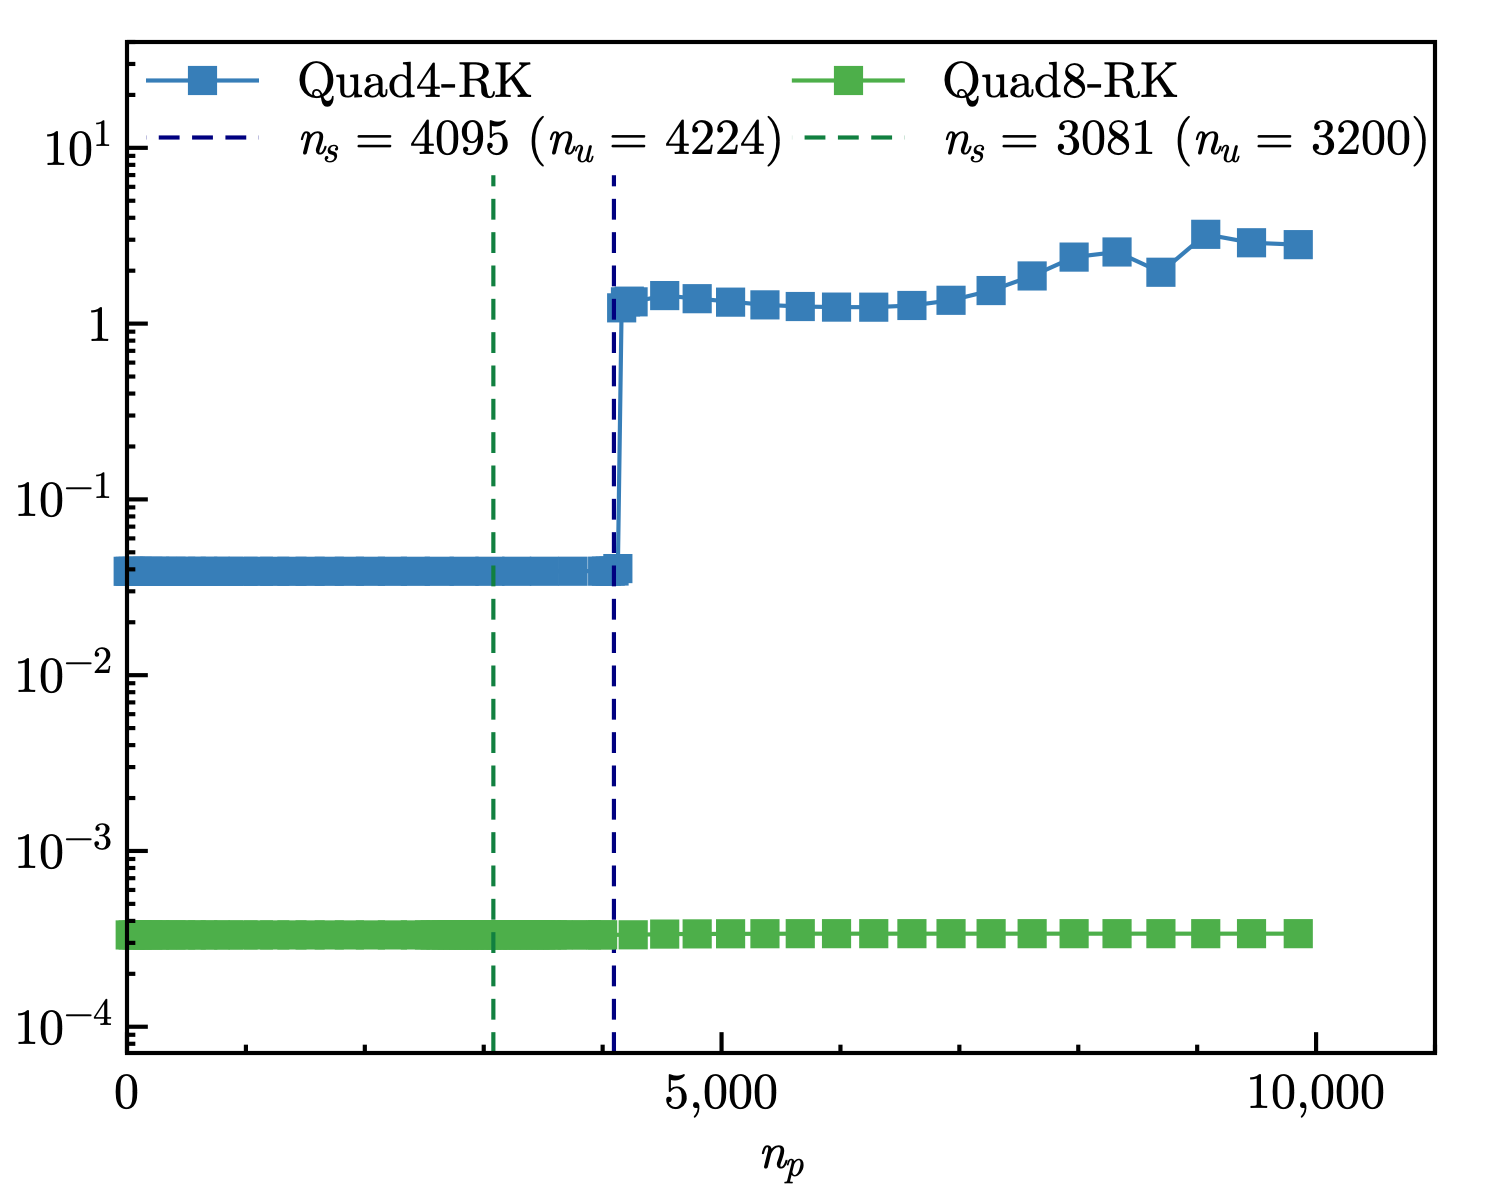
\includegraphics[width=0.48\textwidth]{png/cantilever_Hdev_32.png}}
& \raisebox{-0.85\height}{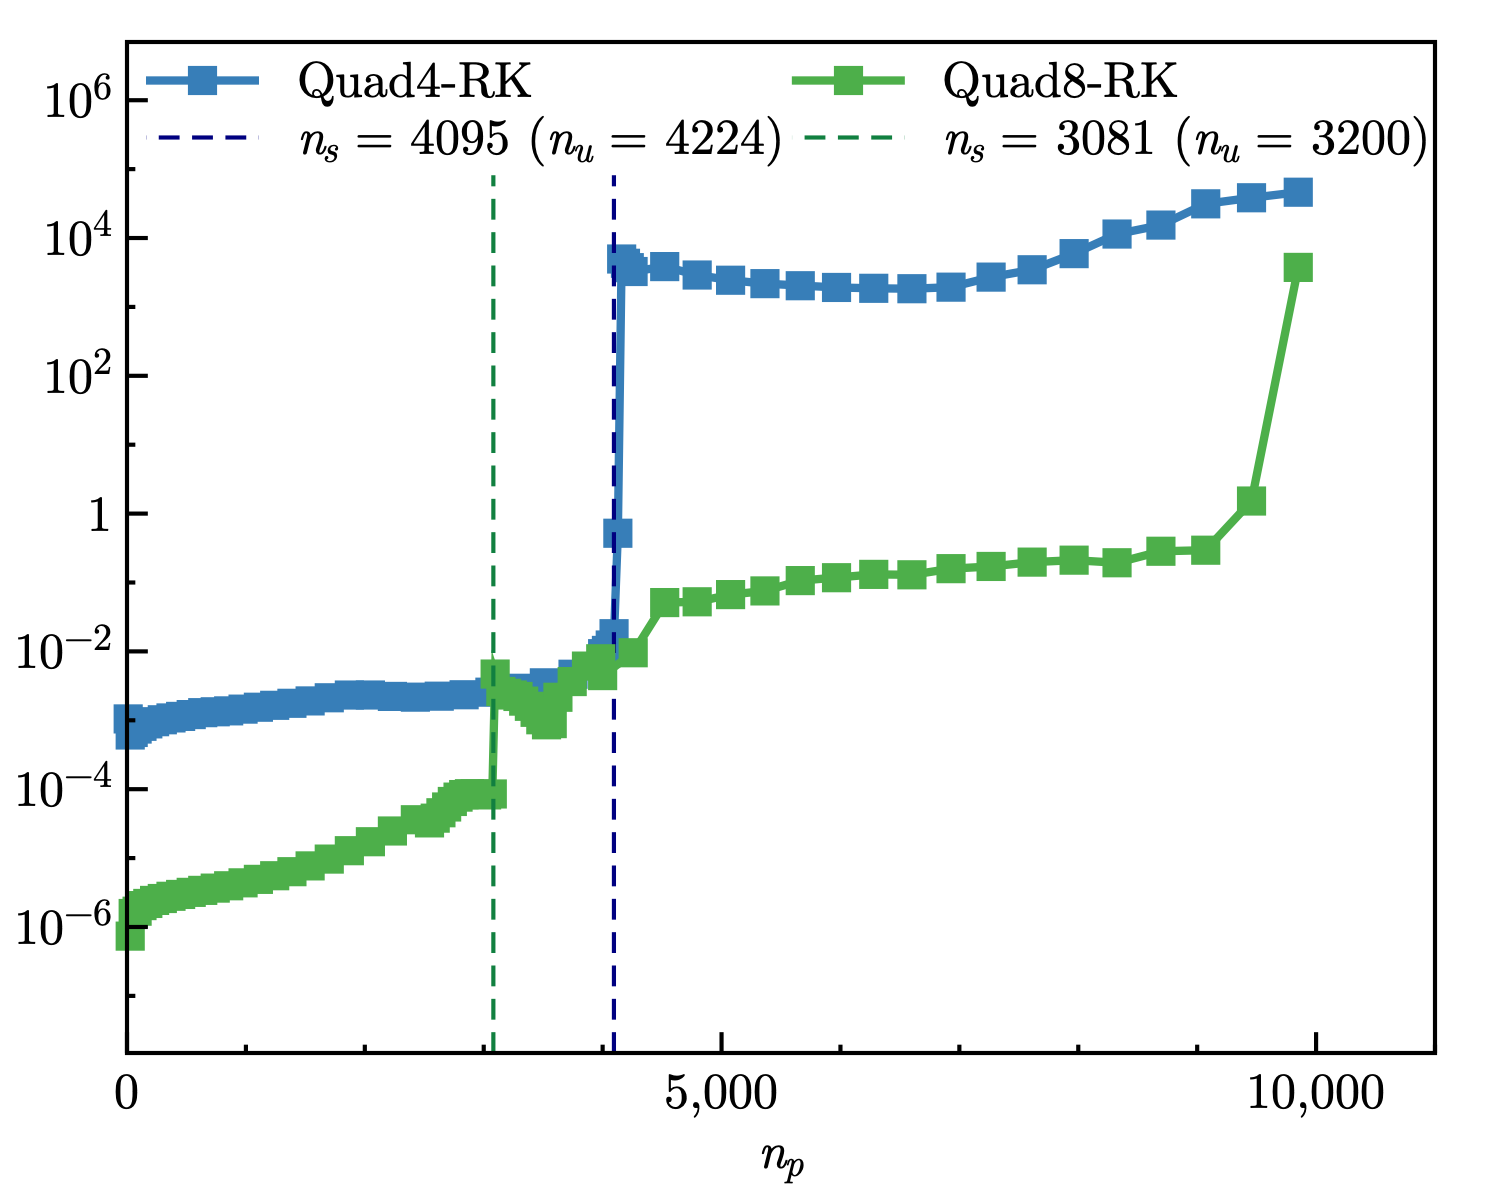
\includegraphics[width=0.48\textwidth]{png/cantilever_L2_p_32.png}} \\
\end{tabular}
\end{subcaptiongroup}
\caption{Strain and pressure errors vs. $n_p$ for cantilever beam problem}\label{fg:cantilever_ns}
\end{figure}

\begin{figure}[H]
\centering
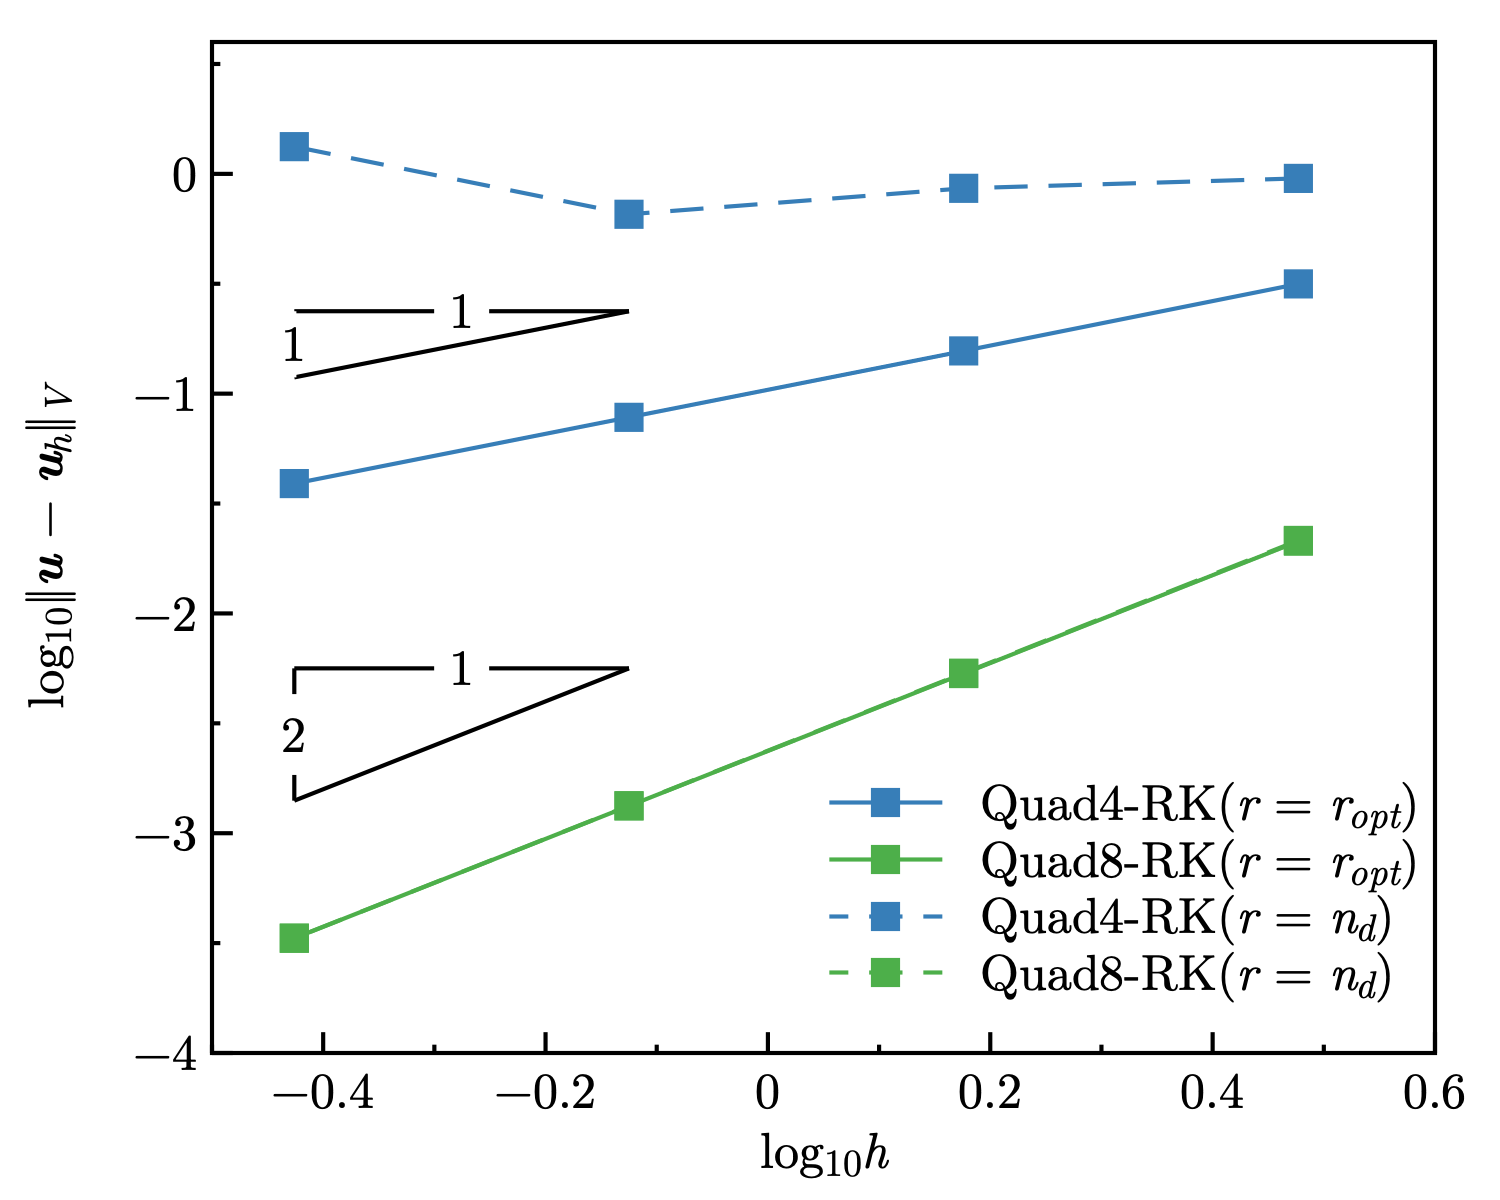
\includegraphics[width=0.49\textwidth]{png/cantilever_Hdev.png}
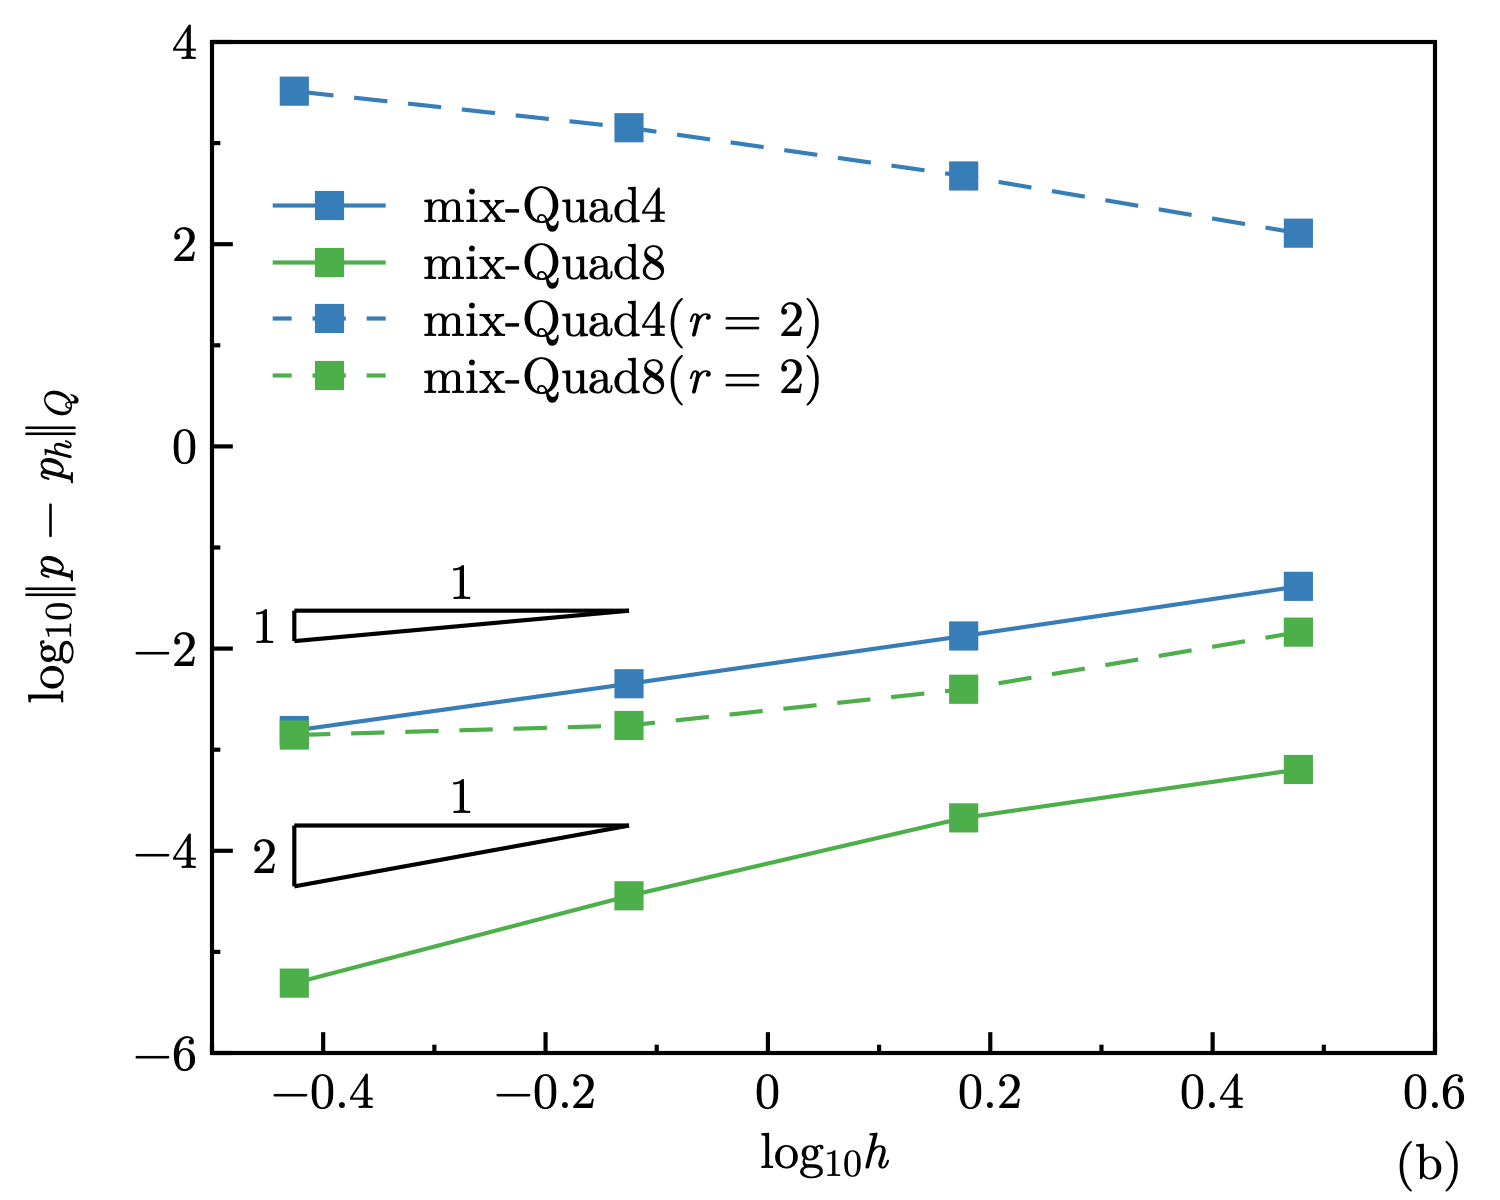
\includegraphics[width=0.49\textwidth]{png/cantilever_L2_p.png}
\caption{Error convergence study for cantilever beam problem: (a) Strain, (b) Pressure}\label{fg:cantilever_convergence}
\end{figure}


\subsection{Plate with hole problem}
Consider an infinite plate with a hole centered at the origin, as shown in Figure \ref{fg:plate_with_hole_model}, and at the infinity towards the $x$-direction subjected to a uniform traction $T=1000$. The geometric and material parameters for this problem are that the ratio of the hole $a=1$, Young's modulus $E=3\times 10^6$, and Poisson's ratio $\nu = 0.5-10^{-8}$. The analytical solution of this problem refers to the Michell solution \cite{timoshenko1969} as:
\begin{equation}\label{plate_with_hole_exact}
\left\{
\begin{aligned}
u_x(\rho,\theta)&=\frac{Ta}{8\mu}\left( \frac{\rho}{a}(k+1)\cos\theta - \frac{2a^3}{\rho^3}\cos3\theta + \frac{2a}{\rho}((1+k)\cos\theta + \cos3\theta) \right) \\
u_y(\rho,\theta)&=\frac{Ta}{8\mu}\left( \frac{\rho}{a}(k-3)\sin\theta - \frac{2a^3}{\rho^3}\sin3\theta + \frac{2a}{\rho}((1-k)\sin\theta + \sin3\theta) \right)
\end{aligned}
\right.
\end{equation}
in which $k = \frac{3-\nu}{1+\nu}$, $\mu = \frac{E}{2(1+\nu)}$. And the stress components are given by:
\begin{equation}
\left\{
\begin{aligned}
\sigma_{xx}&=T\left( 1 - \frac{a^2}{\rho^2}\left( \frac{3}{2}\cos2\theta + \cos4\theta \right) + \frac{3a^4}{2\rho^4}\cos4\theta \right) \\
\sigma_{yy}&=-T\left( \frac{a^2}{\rho^2}\left( \frac{1}{2}\cos2\theta - \cos4\theta \right) + \frac{3a^4}{2\rho^4}\cos4\theta \right) \\
\sigma_{xy}&=-T\left( \frac{a^2}{\rho^2}\left( \frac{1}{2}\sin2\theta + \sin4\theta \right) - \frac{3a^4}{2\rho^4}\sin4\theta \right) \\
\end{aligned}
\right.
\end{equation}

\begin{figure}[h!]
\centering
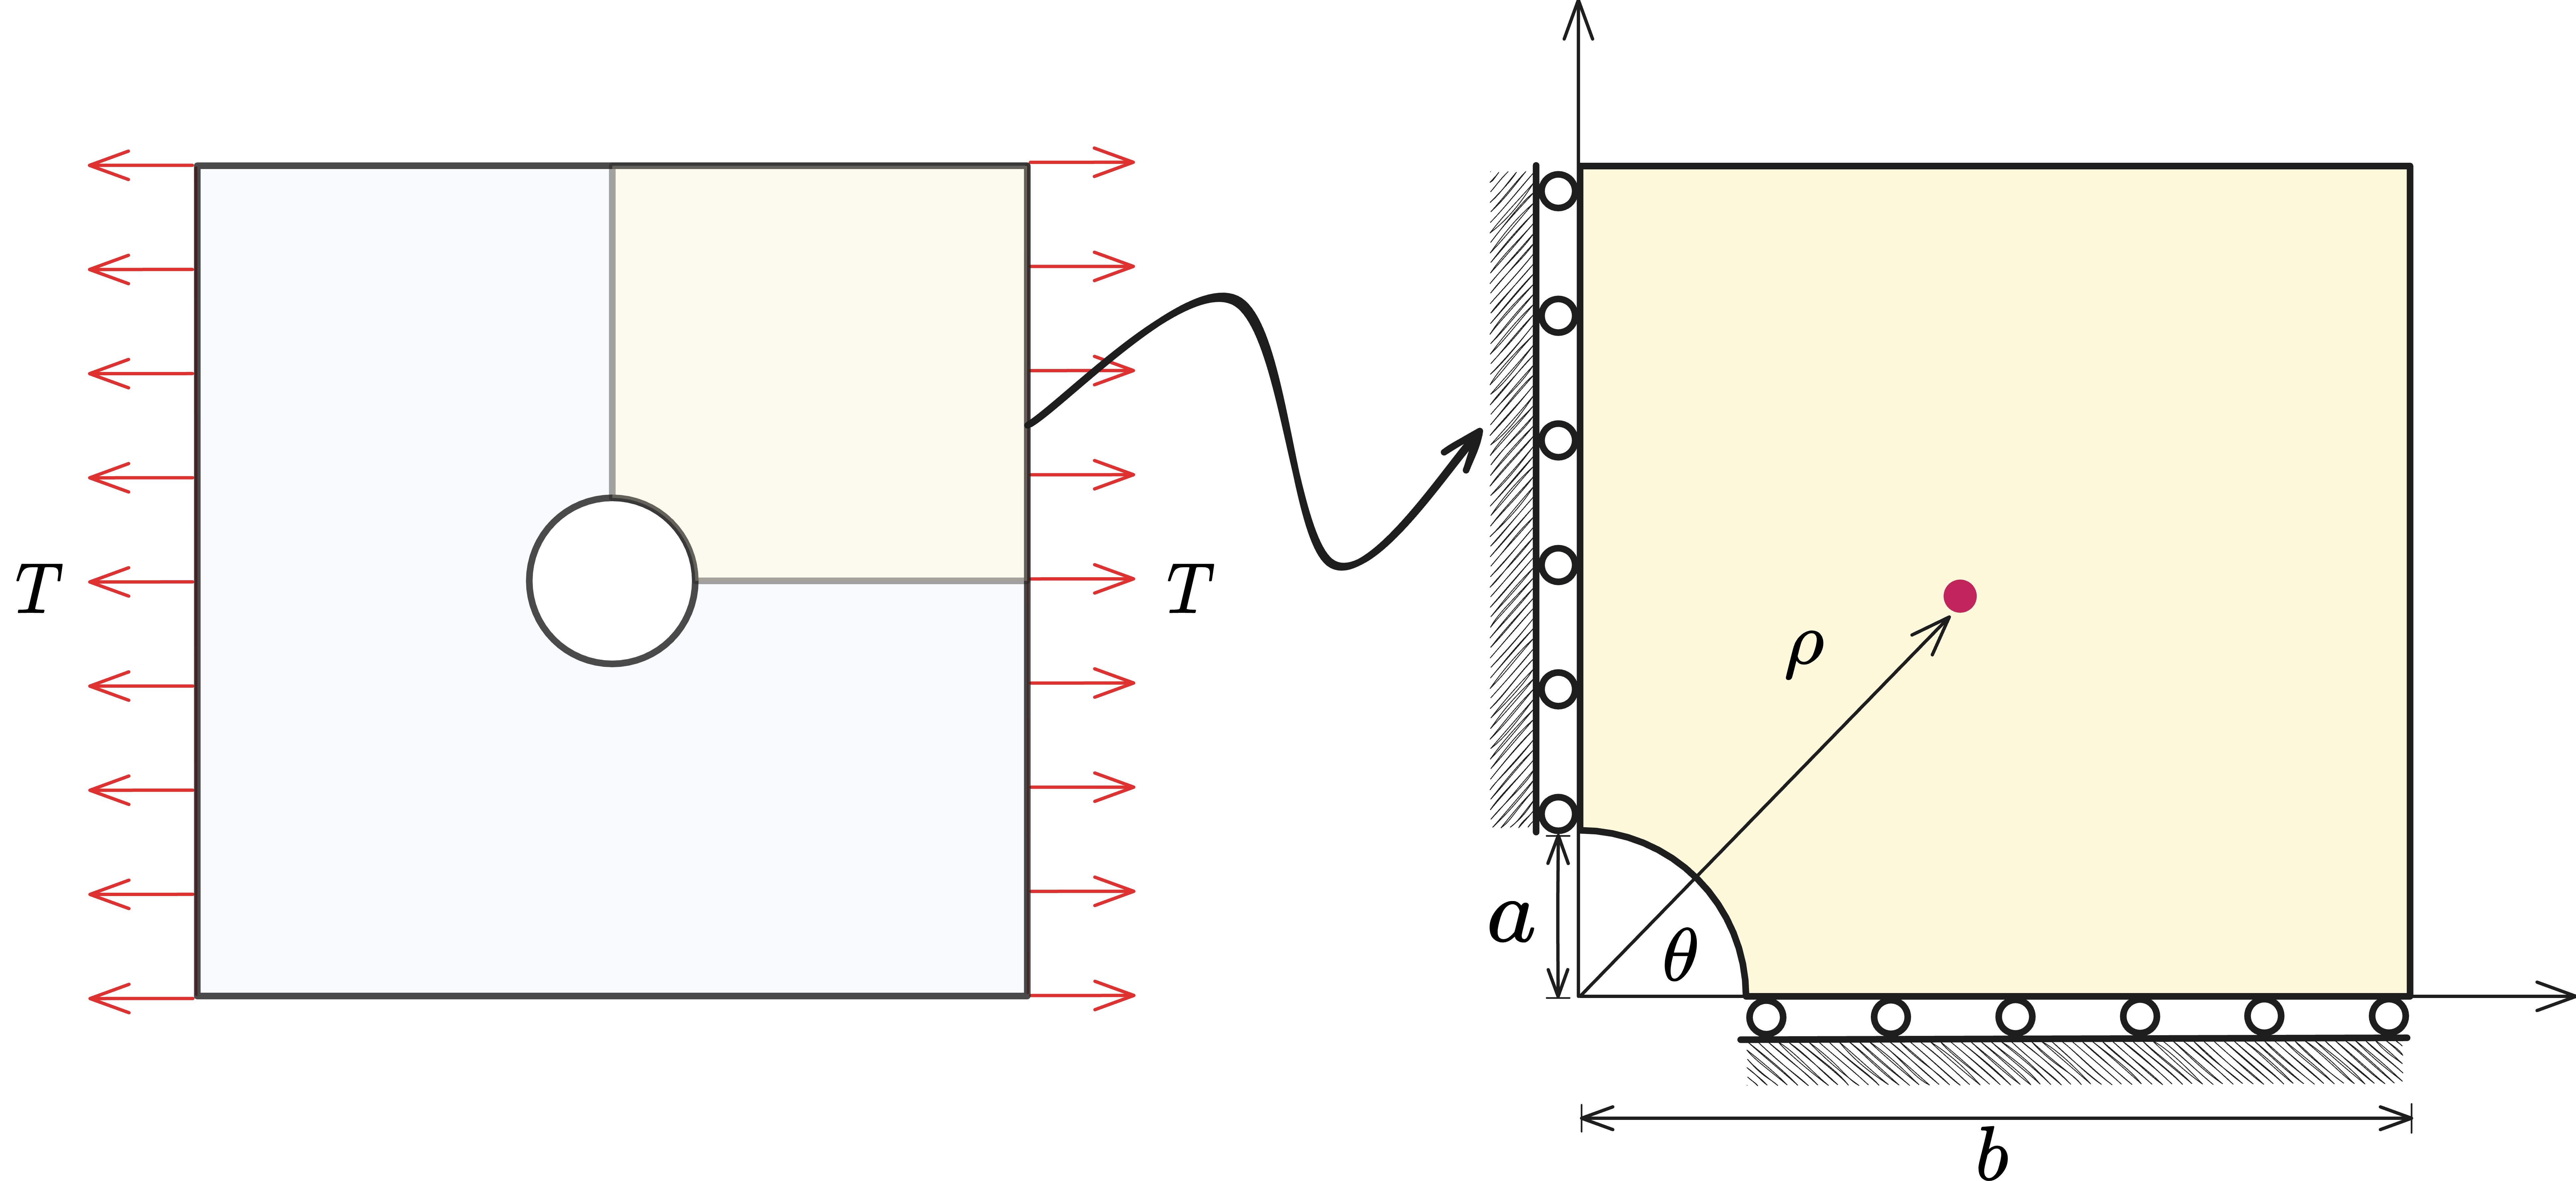
\includegraphics[width=\textwidth]{plate_with_hole_model.png}
\caption{Illustration of plate with hole problem}\label{fg:plate_with_hole_model}
\end{figure}

According to the symmetry property of this problem, only a quarter model with length $b=5$ is considered as shown in Figure \ref{fg:plate_with_hole_model}. The displacement is discretized by 3-node and 6-node triangular elements with $81$, $299$, $1089$, and $4225$ nodes. The corresponding linear and quadratic meshfree formulations are employed for pressure discretization, and the characterized support sizes are chosen as 1.5 and 2.5, respectively.
Figure \ref{fg:plate_with_hole_ns} studies the relationship between strain, pressure errors, and $n_p$ using the nodal distributions uniformly related to displacement nodes.
Unlike the quadrilateral element case in Section \ref{sec:cantilever}, the quadratic Tri6--RK shows worse results while the constraint ratio is out of the optimal range. And Tri3--RK exhibits less sensitivity in strain error than Tri6--RK, but its error is increasing while $n_p$ goes up. Both Tri3--RK and Tri6--RK with constraint ratios under the optimal range perform acceptably. 
The corresponding error convergence study is presented in Figure \ref{fg:plate_with_hole_convergence}, the traditional MINI element and the 6--node triangular displacement element with 3--node continuous triangular pressure element (T6C3) are employed for comparison. The results show that only Tri3--RK with $r=2$ shows a comparable result with the optimal one with $r=r_{opt}$. The other formulations with the traditional constraint ratio show lower accuracy and error convergence rates.

\begin{figure}[H]
\centering
\begin{tabular}{c@{\hspace{0pt}}c}
$\Vert \boldsymbol{u} - \boldsymbol{u}_h \Vert_V$ & $\Vert p - p_h \Vert_Q$ \\
\raisebox{-0.7\height}{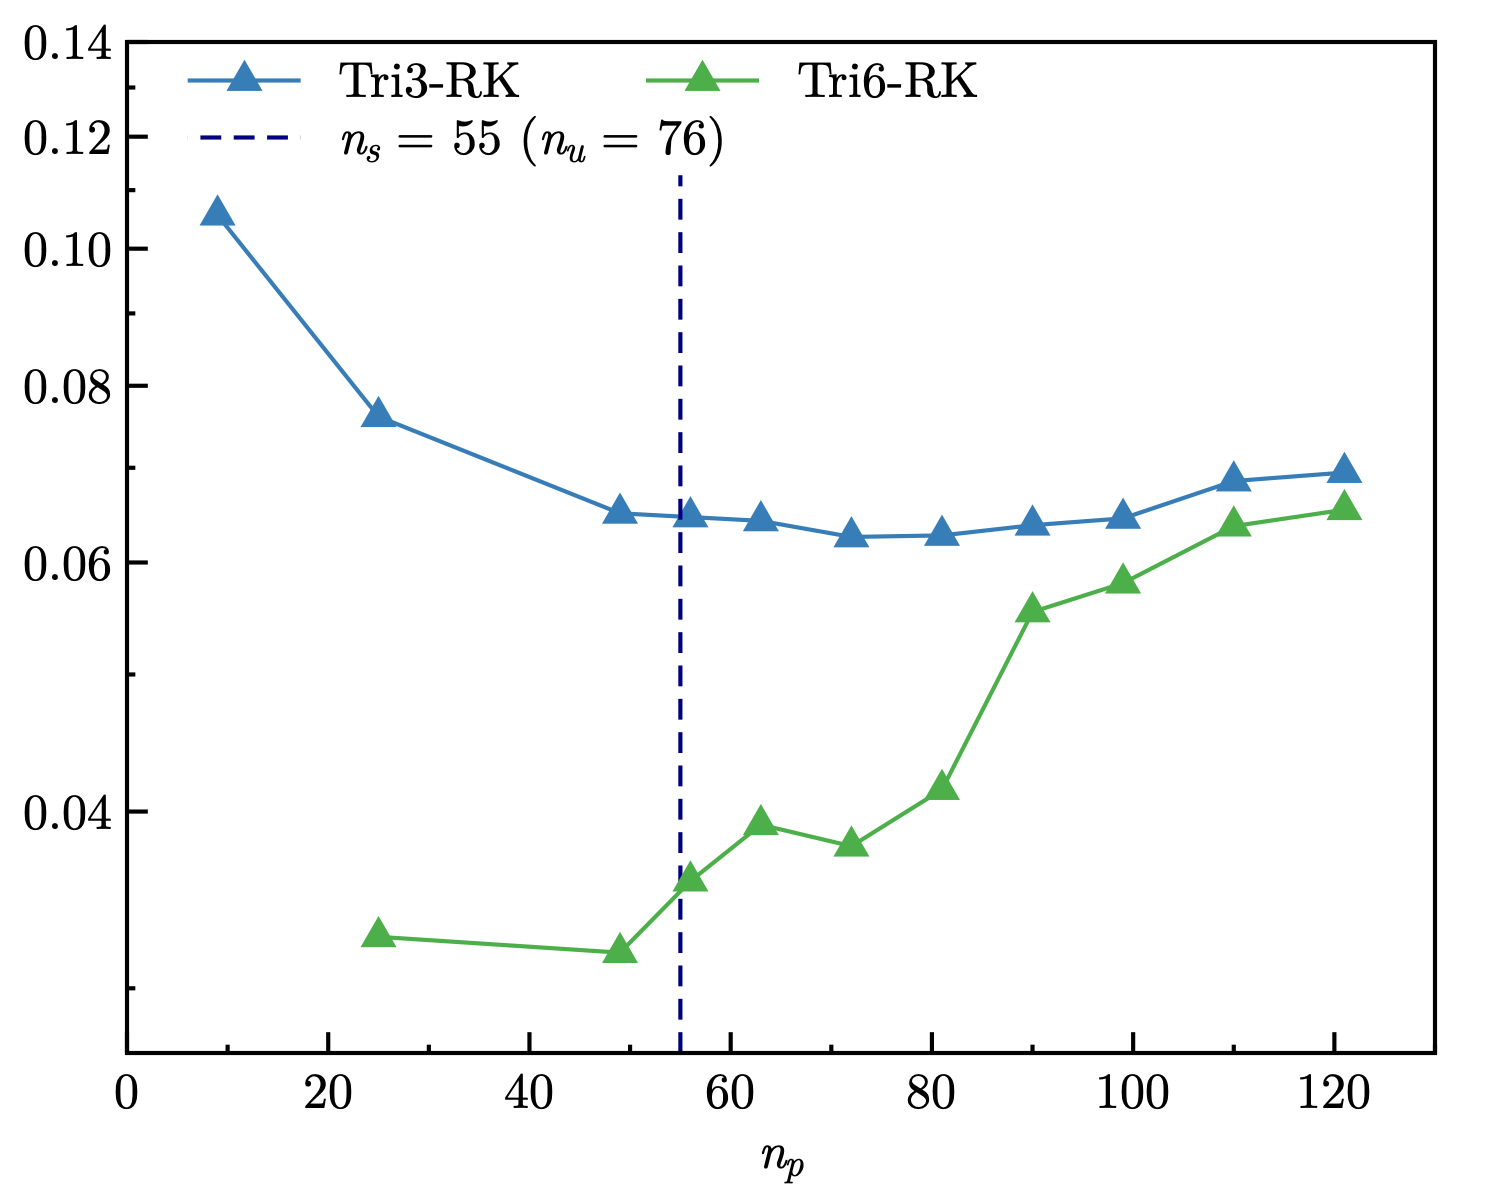
\includegraphics[width=0.48\textwidth]{plate_Hdev_4.png}}
& \raisebox{-0.7\height}{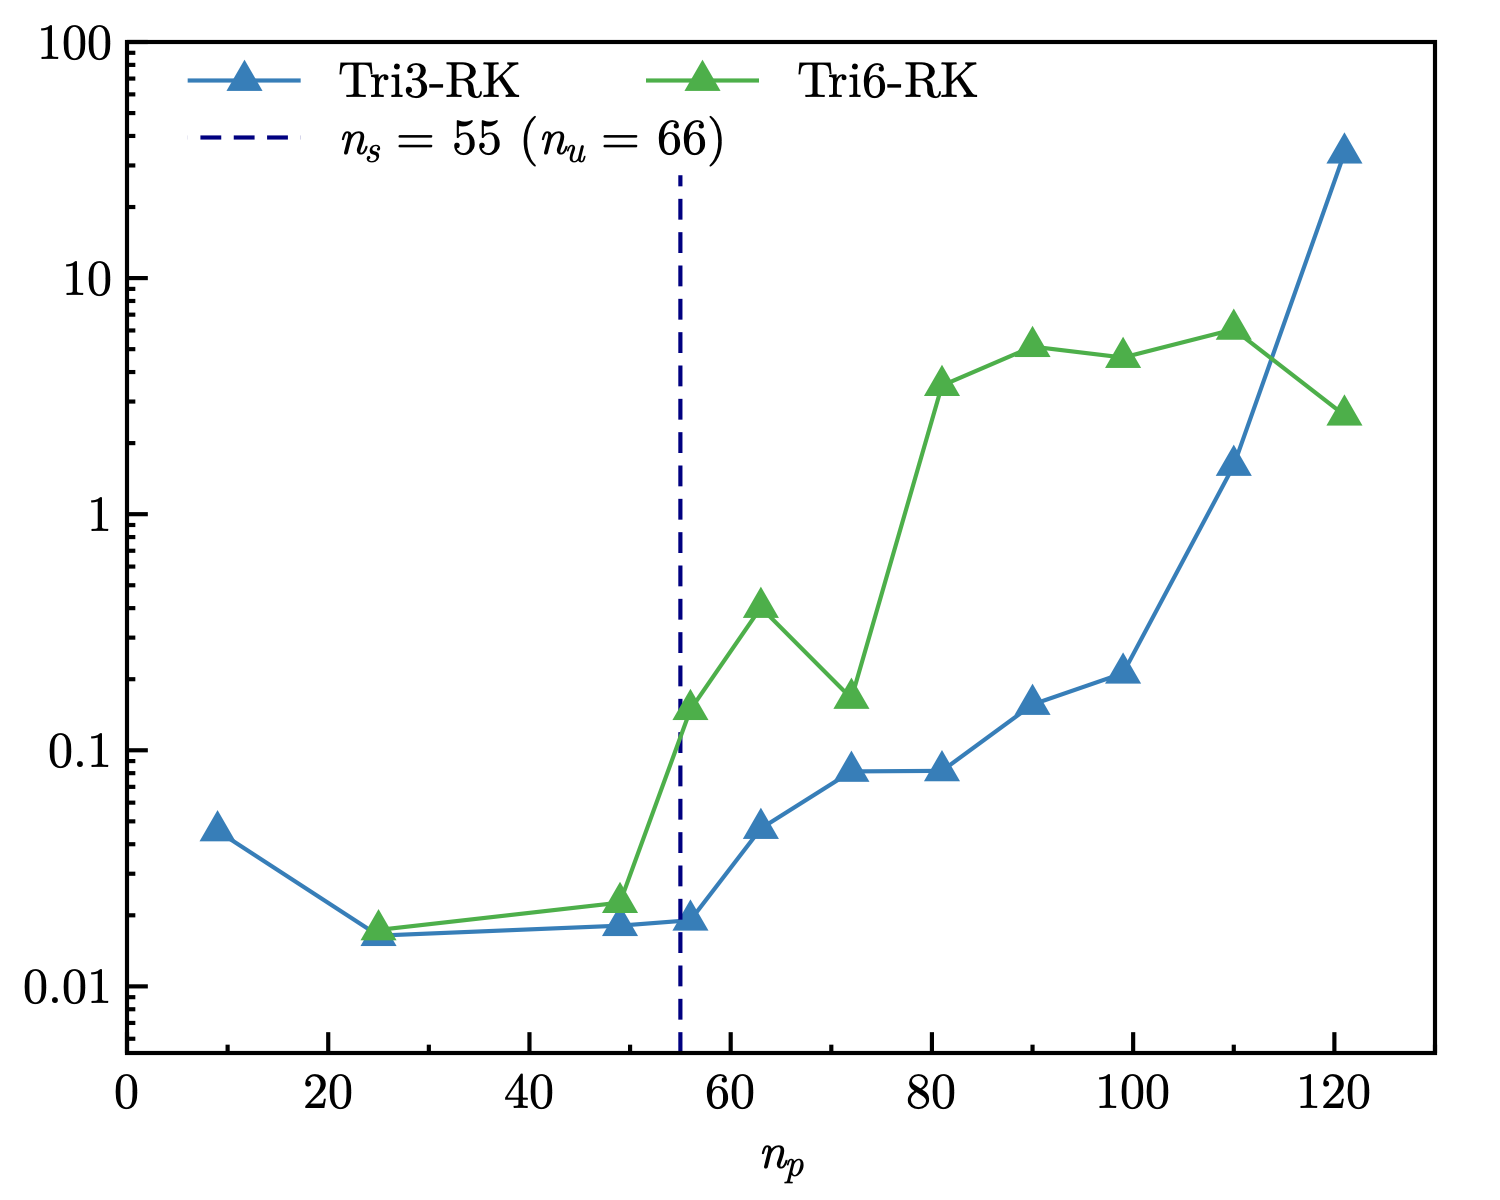
\includegraphics[width=0.48\textwidth]{plate_L2_p_4.png}} \\
\raisebox{-0.7\height}{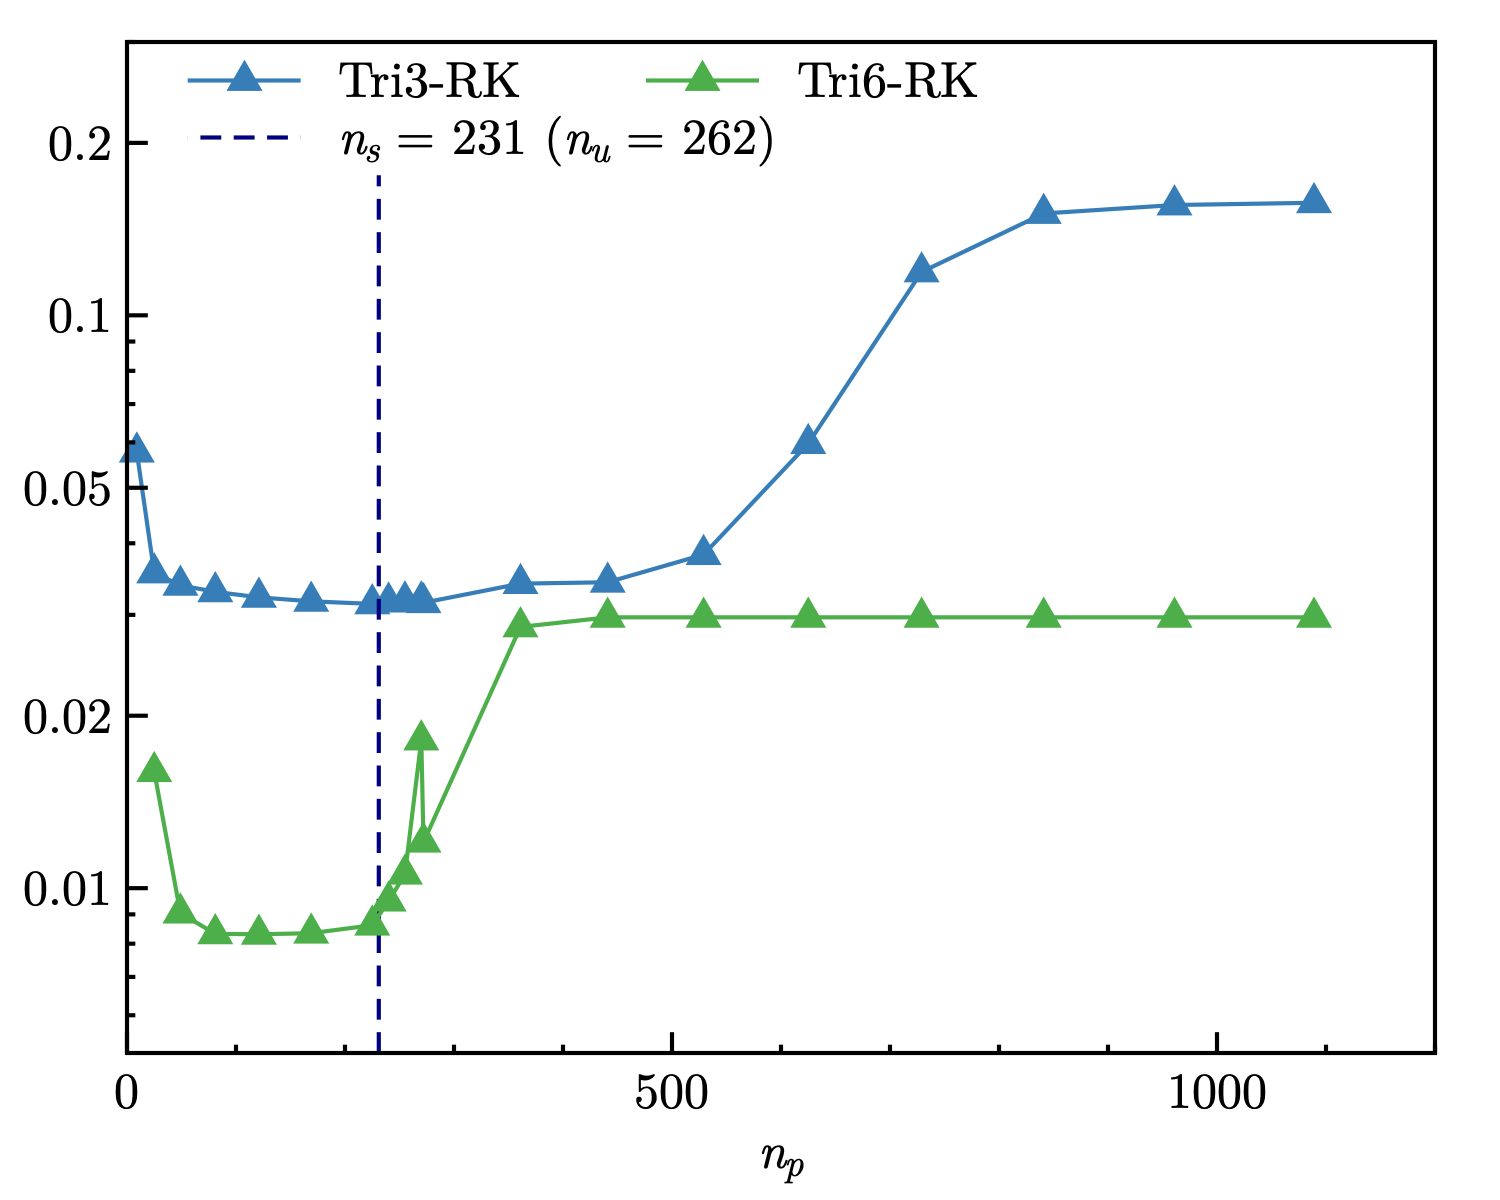
\includegraphics[width=0.48\textwidth]{plate_Hdev_8.png}}
& \raisebox{-0.7\height}{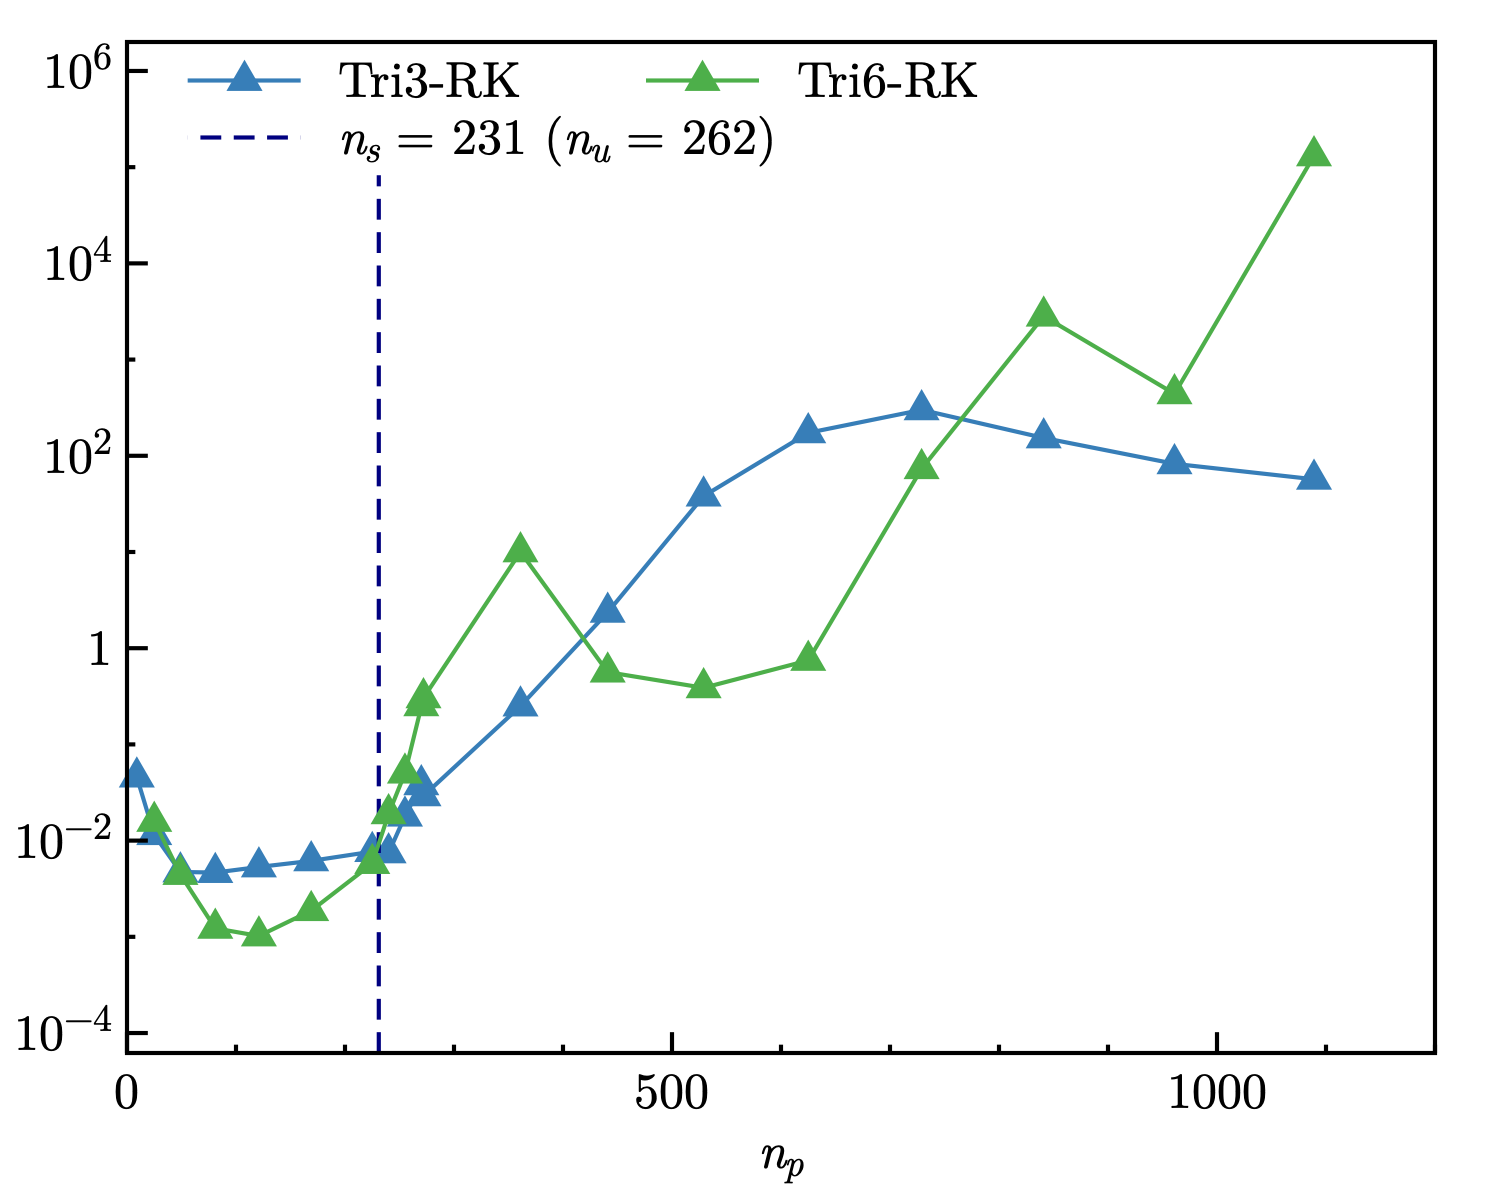
\includegraphics[width=0.48\textwidth]{plate_L2_p_8.png}} \\
\raisebox{-0.7\height}{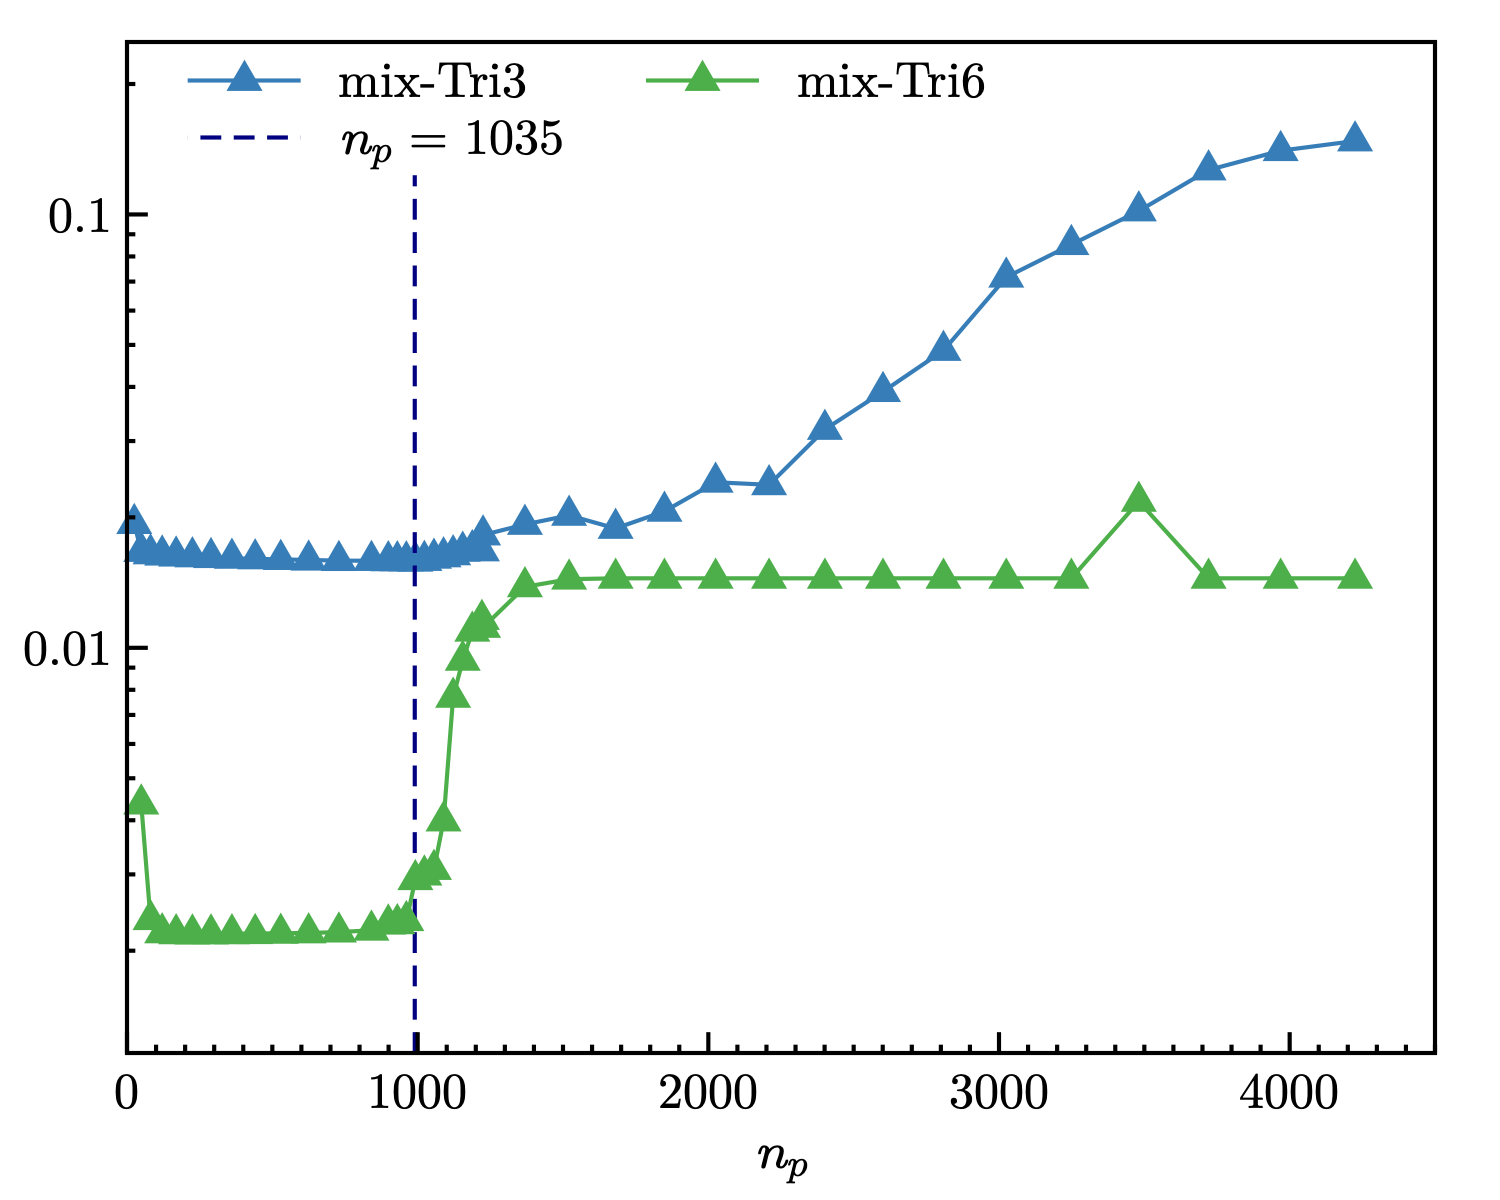
\includegraphics[width=0.48\textwidth]{plate_Hdev_16.png}}
& \raisebox{-0.7\height}{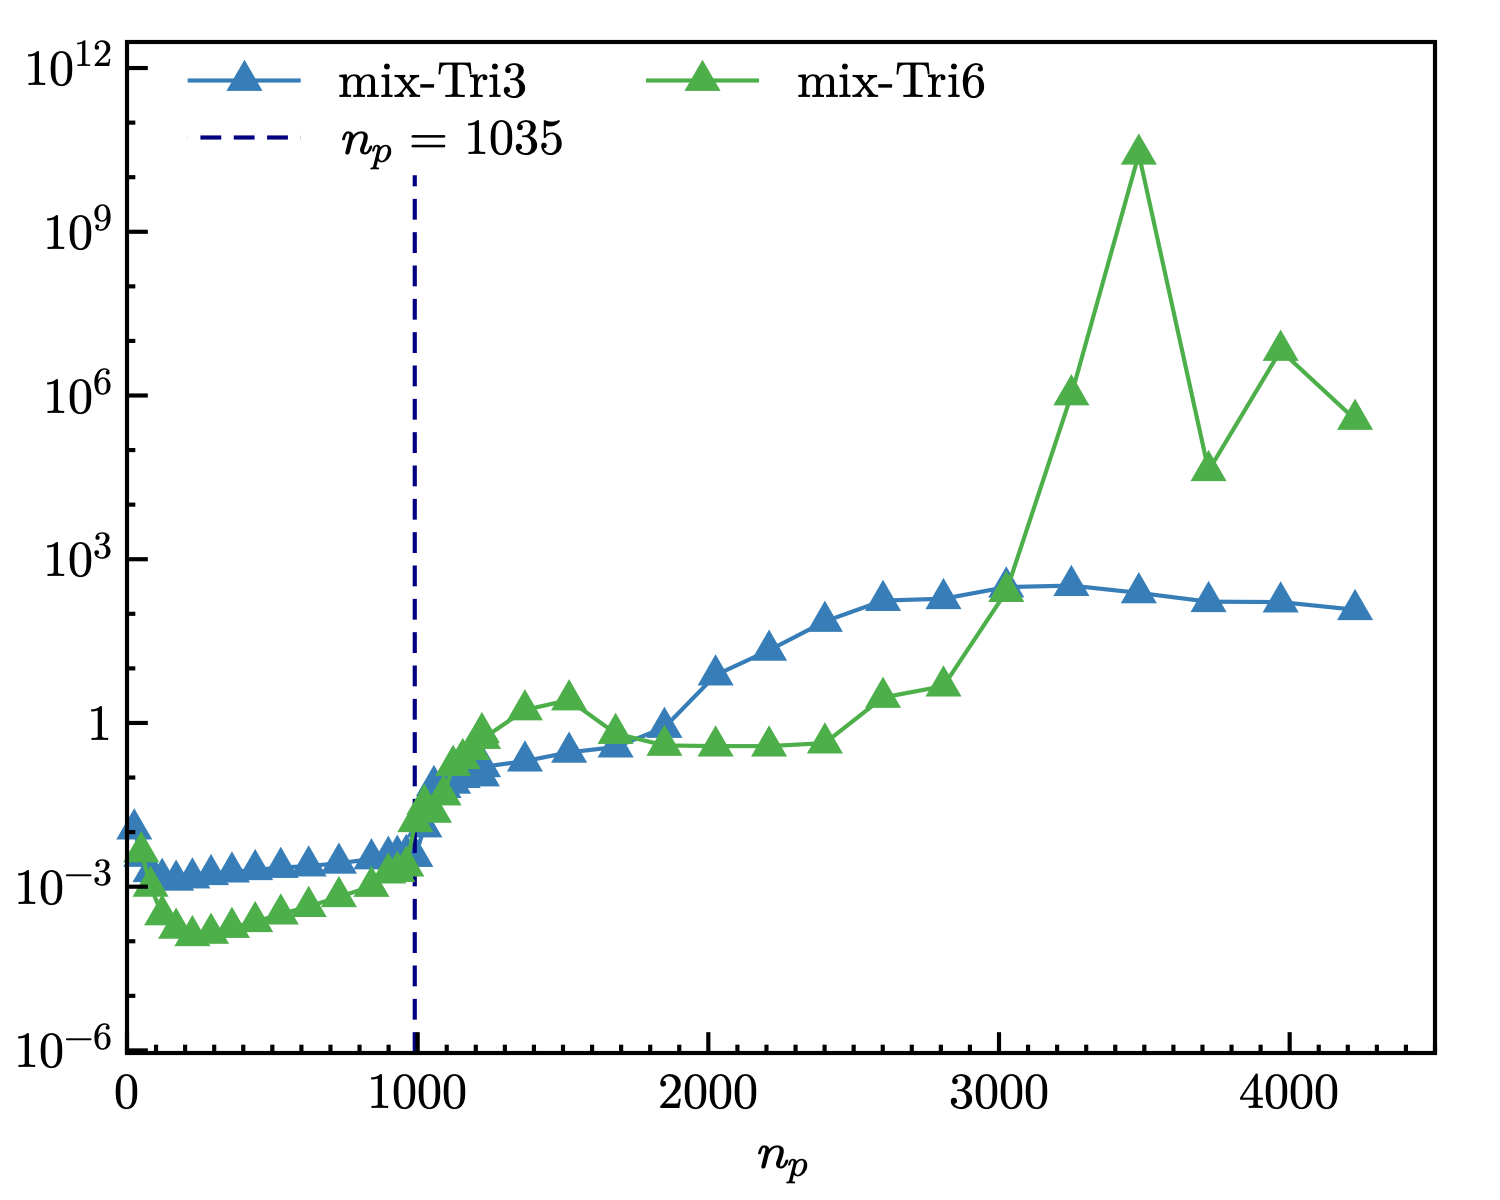
\includegraphics[width=0.48\textwidth]{plate_L2_p_16.png}} \\
\raisebox{-0.7\height}{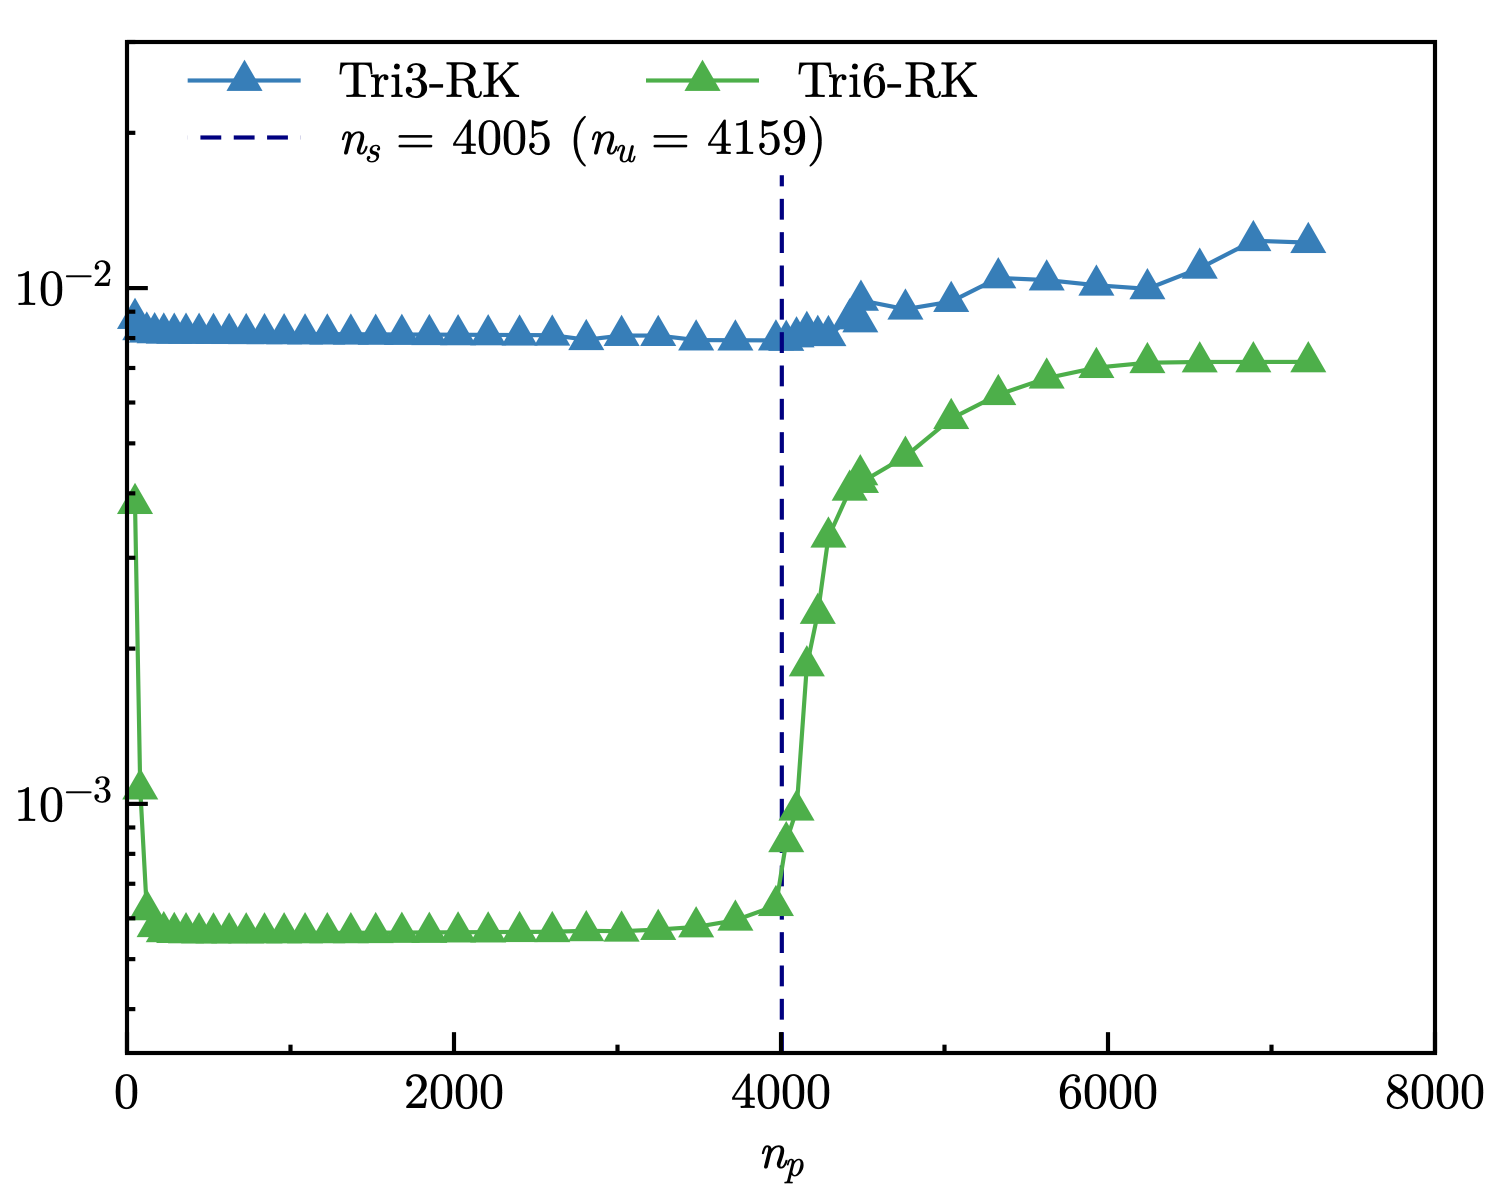
\includegraphics[width=0.48\textwidth]{plate_Hdev_32.png}}
& \raisebox{-0.7\height}{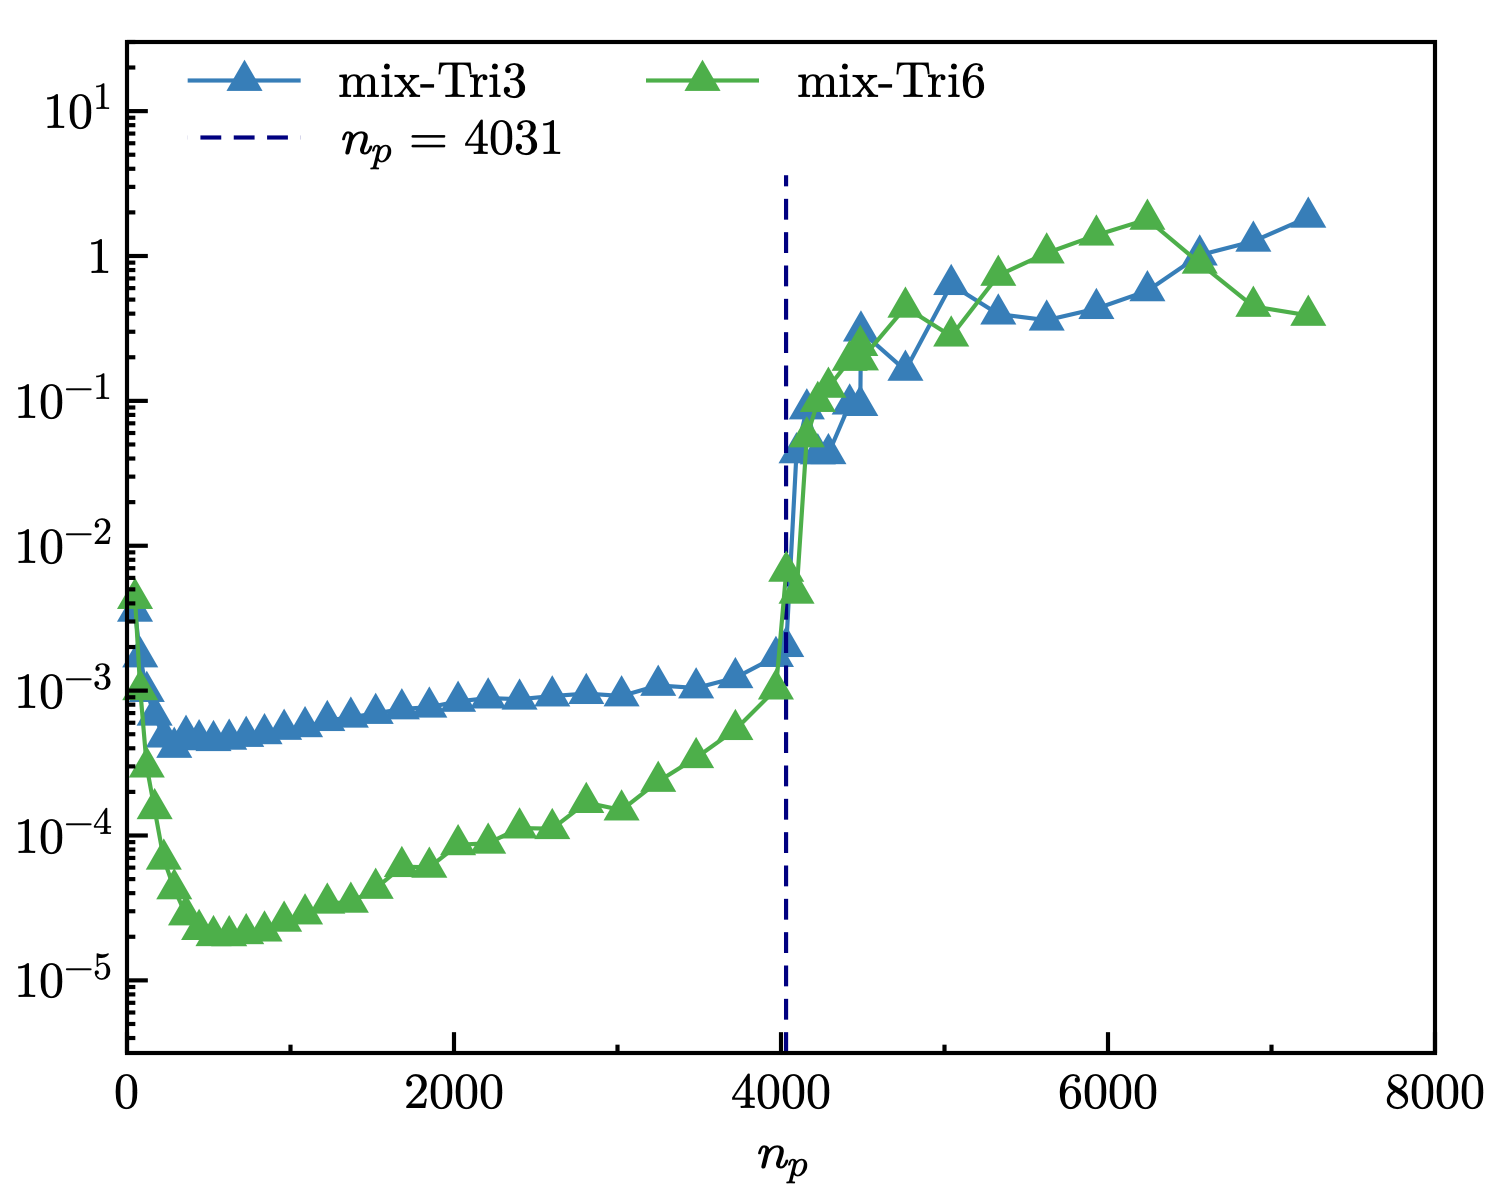
\includegraphics[width=0.48\textwidth]{plate_L2_p_32.png}} \\
\end{tabular}
\caption{Strain and pressure errors vs. $n_p$ for plate with hole problem}\label{fg:plate_with_hole_ns}
\end{figure}

\begin{figure}[H]
\centering
\begin{subcaptiongroup}
\centering
\parbox[b]{0.49\textwidth}{
    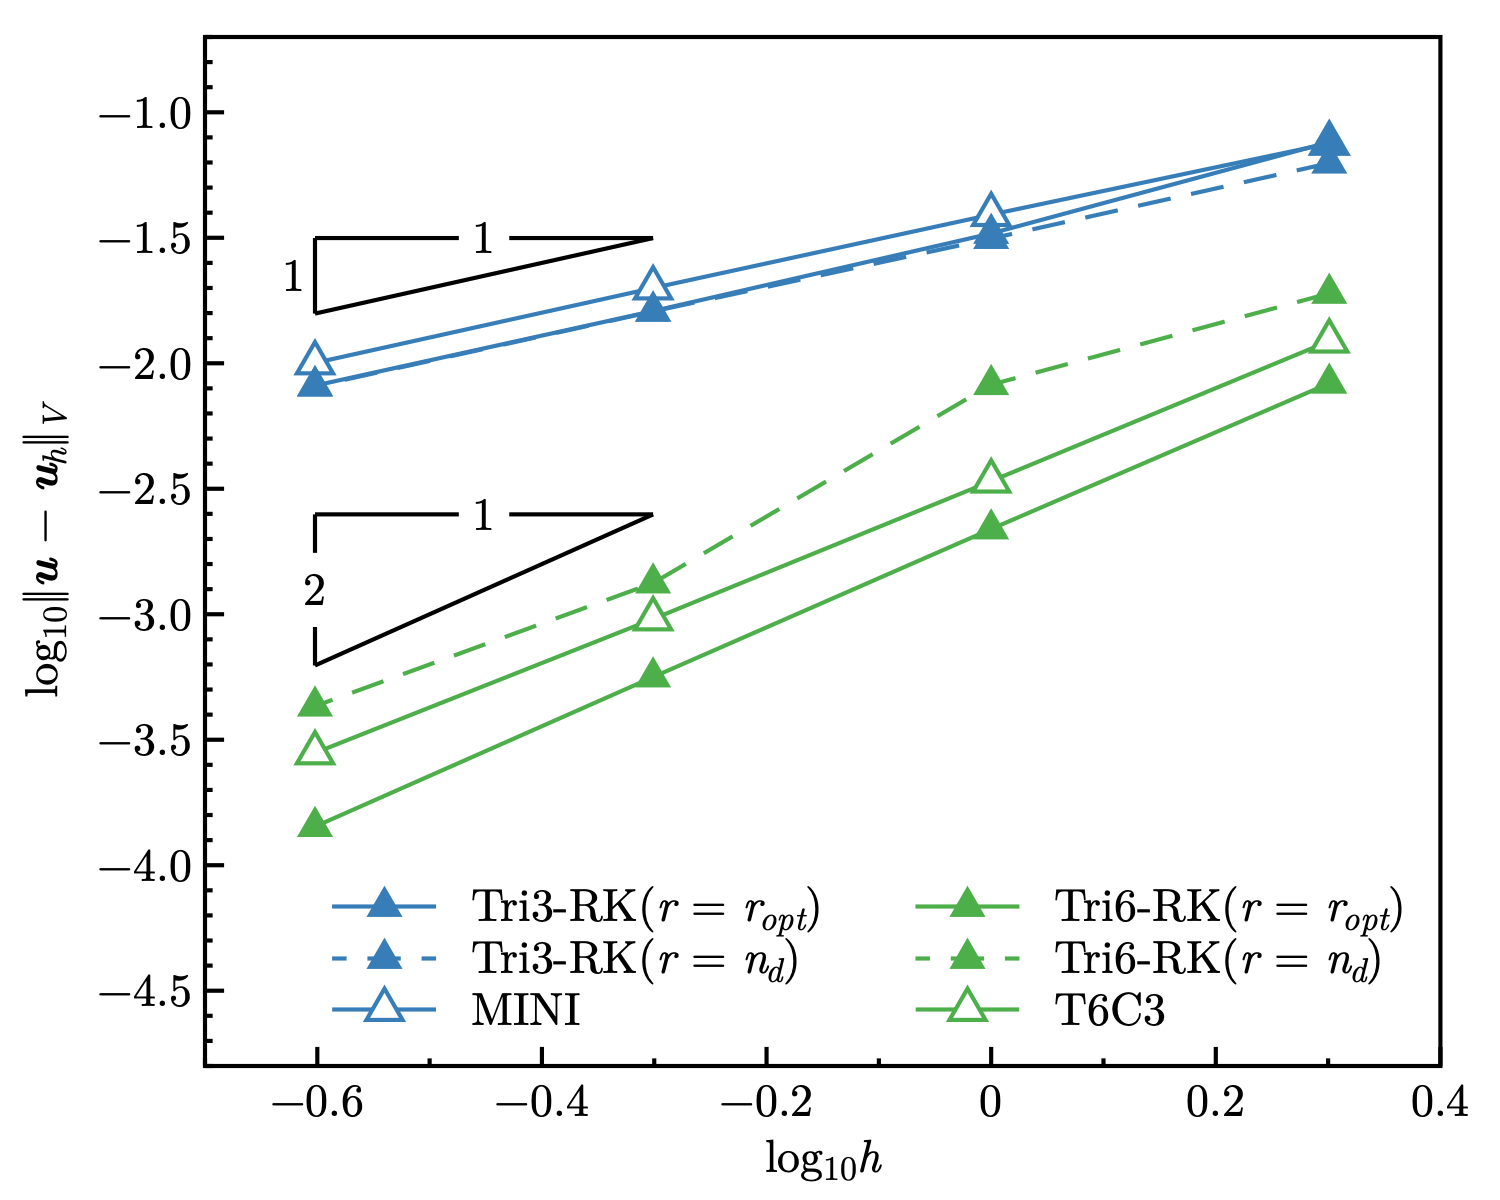
\includegraphics[width=0.49\textwidth]{plate_with_hole_Hdev_r1.png}
    \caption{Strain error}\label{fg:plate_with_hole_convergence_strain}
}
\parbox[b]{0.49\textwidth}{
    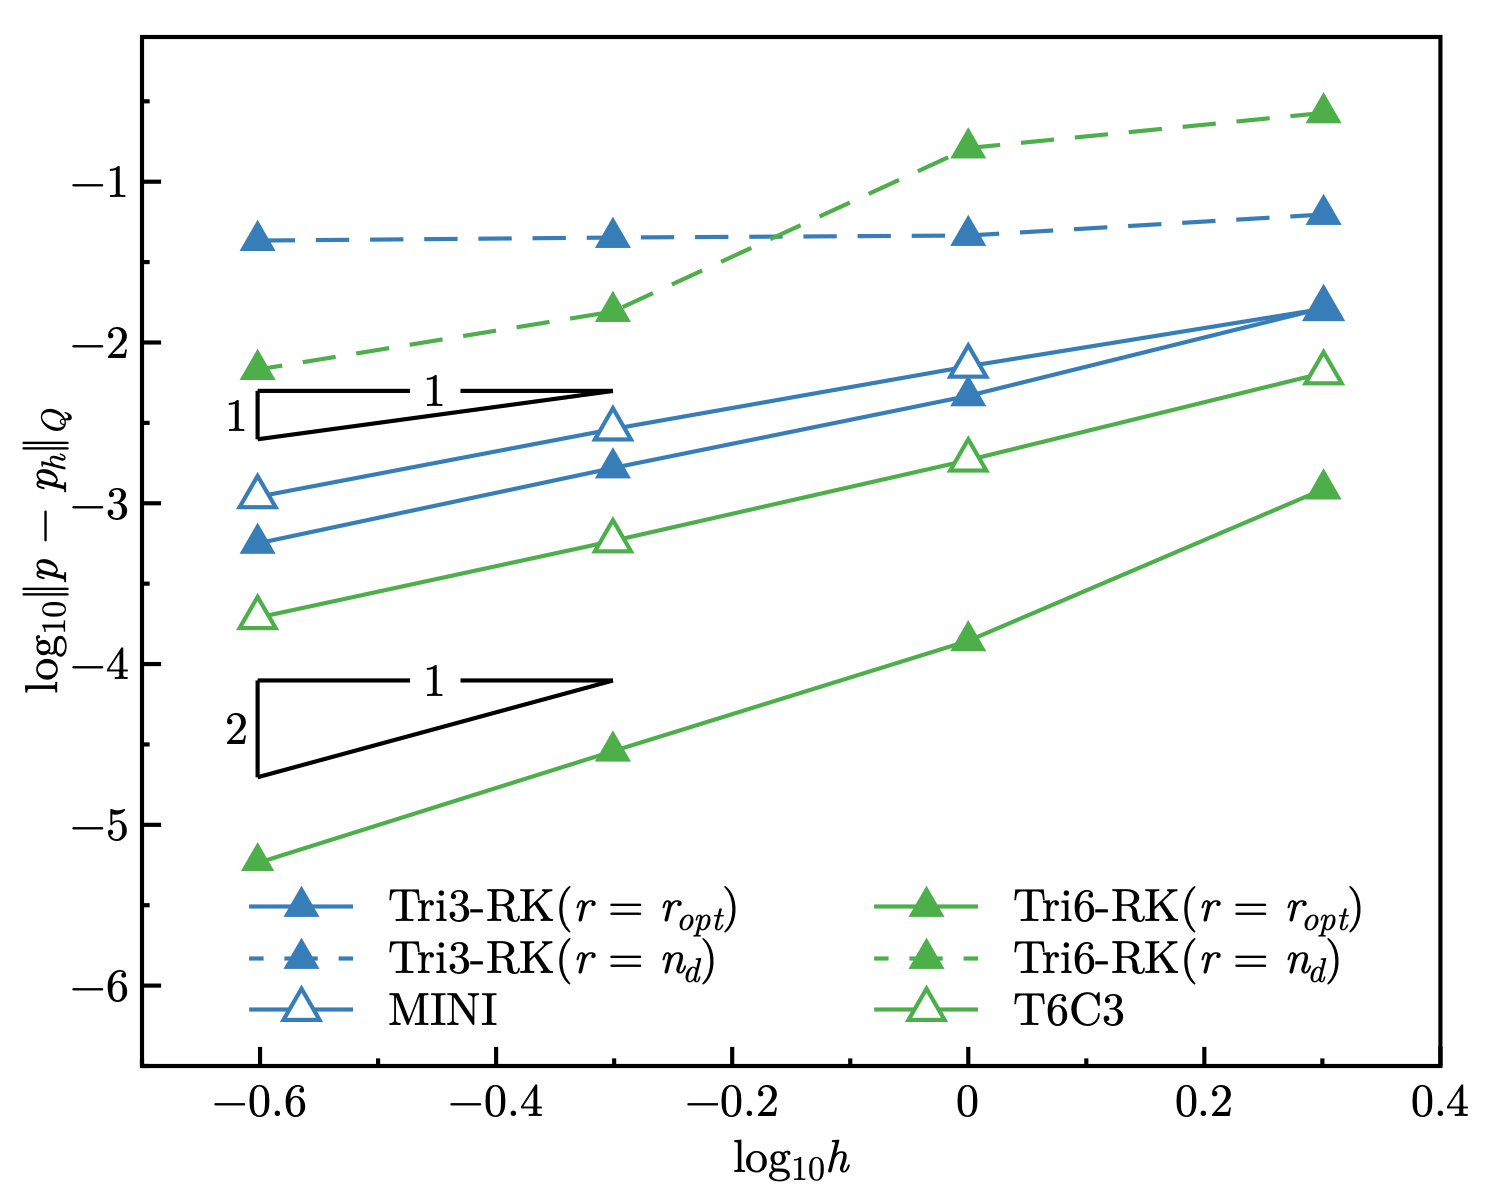
\includegraphics[width=0.49\textwidth]{plate_with_hole_L2_p_r1.png}
    \caption{Pressure error}\label{fg:plate_with_hole_convergence_pressure}
}
\end{subcaptiongroup}
\caption{Error convergence study for plate with a hole problem}\label{fg:plate_with_hole_convergence}
\end{figure}


% \subsection{Cook membrane problem}

The Cook membrane problem \cite{simo1990} is used herein for stability analysis of pressure. The geometry of this problem is shown in Figure \ref{fg:cook_illsutration}, in which the left hand side is fixed and the right hand side subjects a concentrated force $P=6.25$ in the $y$-direction. The material parameters are Young's modulus $E=70.0$ and Poisson's ratio $\nu=0.5-10^{-8}$.

\begin{figure}[H]
\centering
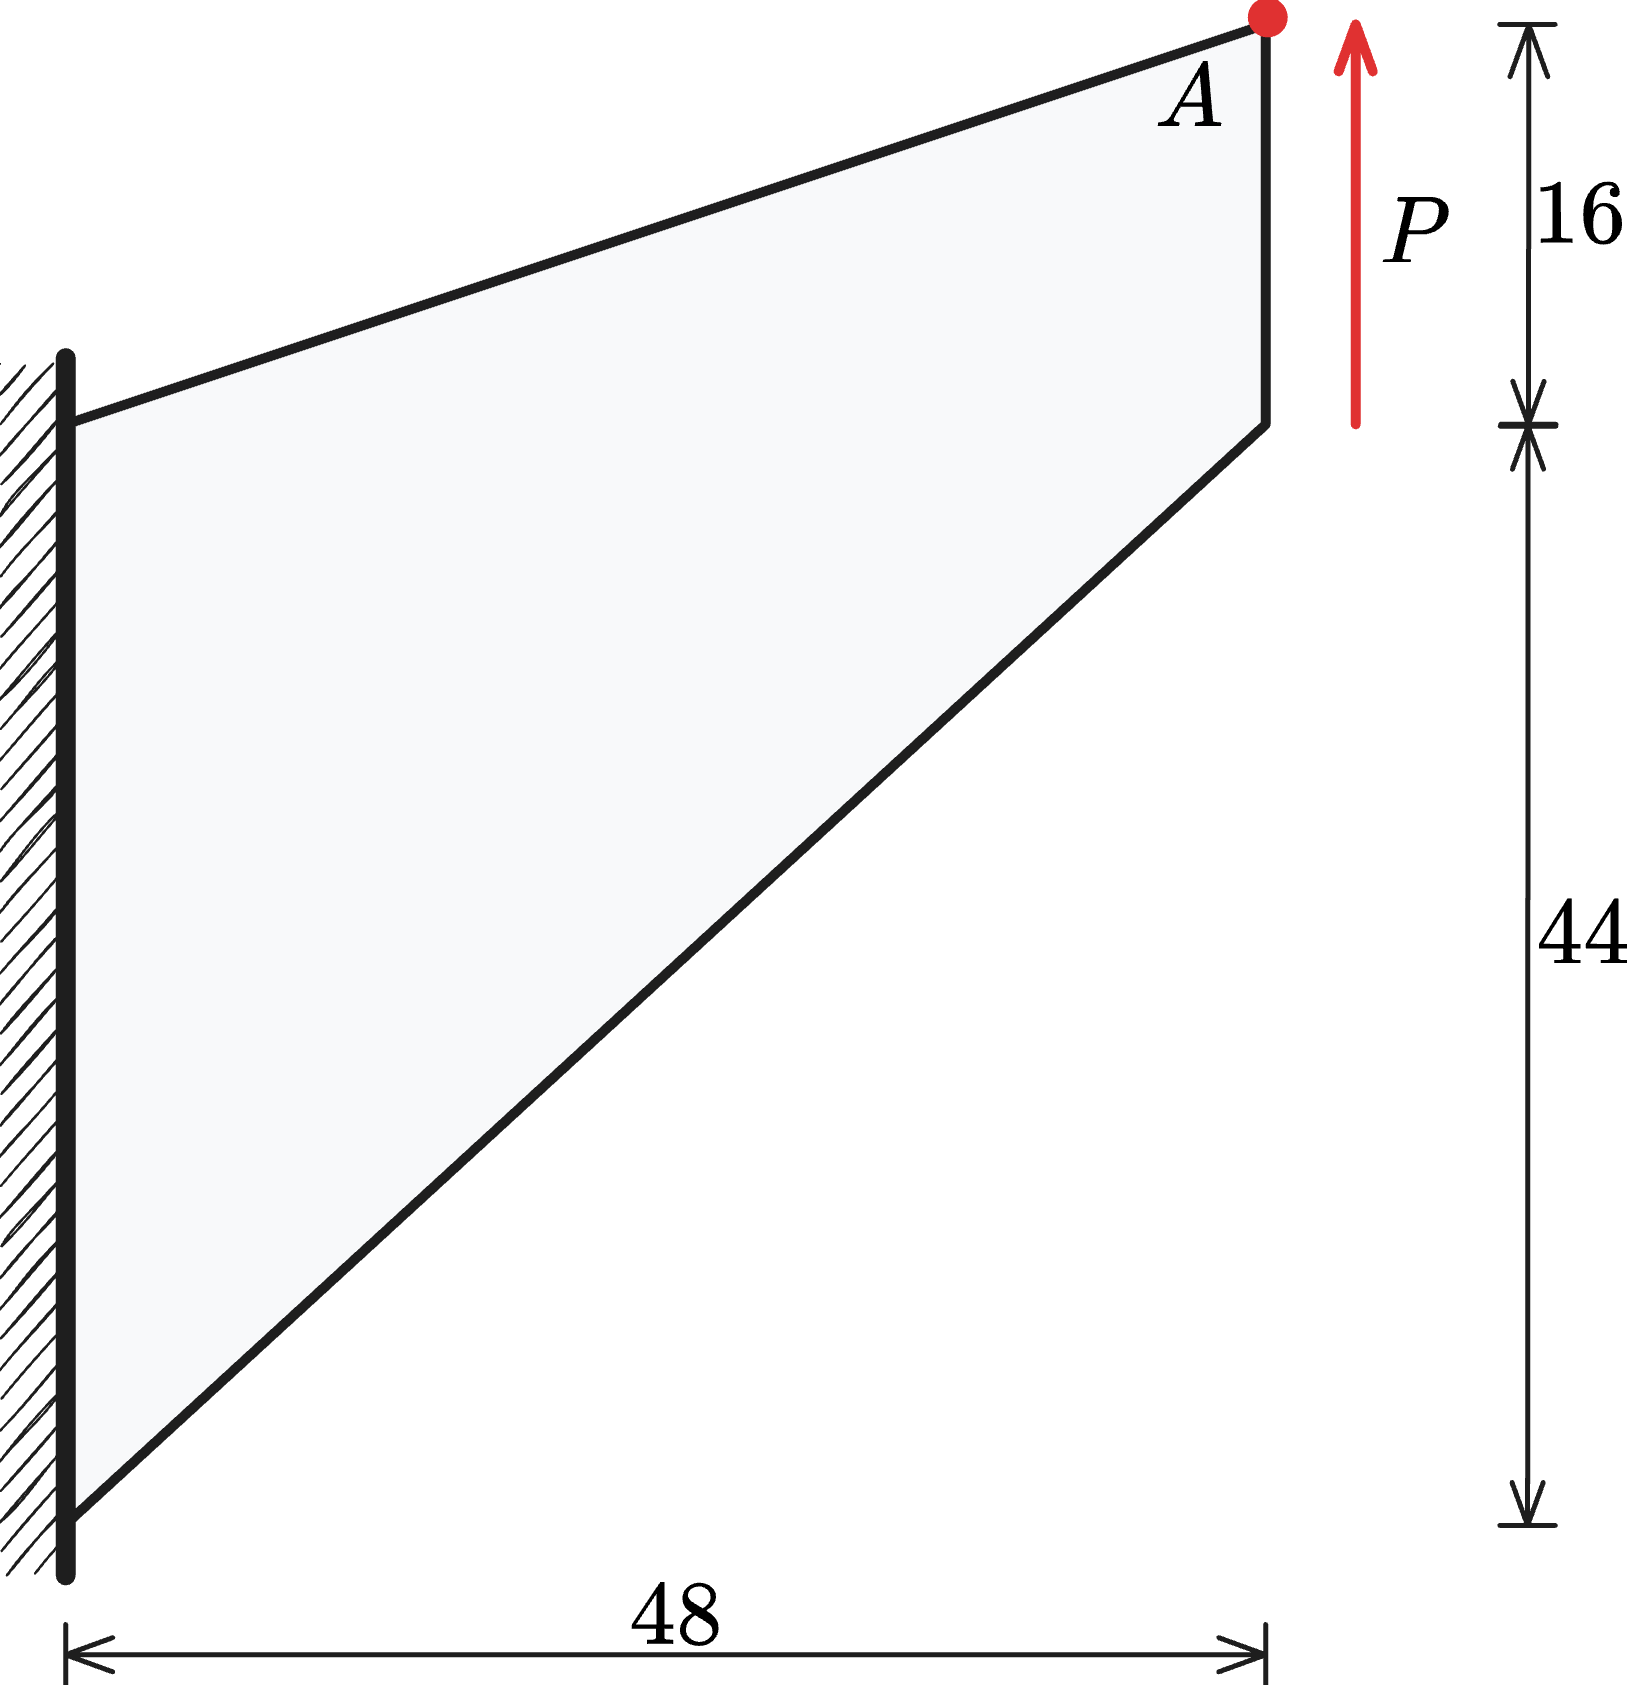
\includegraphics[width=0.5\textwidth]{png/cook_membrane_model.png}
\caption{Illustration of Cook membrane problem}\label{fg:cook_illsutration}
\end{figure}

In this test, we focus on the pressure stability of 2D mixed FE--meshfree formulations. Figures \ref{fg:cook_membrane_contour_tri3}--\ref{fg:cook_membrane_contour_quad8} show the pressure contour plots for non-uniform Tri3--RK, Tri6--RK, Quad4--RK, and Quad8--RK formulations with $r=n_d$ and $r=r_{opt}$, respectively. The reproducing kernel meshfree approximations are employed for pressure discretization with characterized support sizes of 1.5 for the linear basis function and 2.5 for the quadratic basis function. The results imply that the pressure contour plots with the optimal constraint ratio $r=r_{opt}$ show a more stable and smooth pressure distribution compared to those with the traditional constraint ratio $r=n_d$.

\begin{figure}[H]
\centering
\begin{tabular}{c@{\hspace{5pt}}c@{\hspace{5pt}}c@{\hspace{5pt}}c}
\includegraphics[width=0.33\textwidth]{png/cook_mix_tri3_mesh_2529.png}
& \includegraphics[width=0.28\textwidth]{png/cook_tri3_2529_2529.png}
& \includegraphics[width=0.28\textwidth]{png/cook_tri3_2529_658.png}
& \includegraphics[width=0.1\textwidth]{png/legend.png} \\
$n_u = 2529$ & $r = n_d$ & $r = r_{opt}$ &
\end{tabular}
\caption{Pressure contour plots for Cook membrane problem using Tri3--RK}\label{fg:cook_membrane_contour_tri3}
\end{figure}

\begin{figure}[H]
\centering
\begin{tabular}{c@{\hspace{5pt}}c@{\hspace{5pt}}c@{\hspace{5pt}}c}
\includegraphics[width=0.33\textwidth]{png/cook_tri6_2529_msh.png}
& \includegraphics[width=0.28\textwidth]{png/cook_tri6_2529_2529.png}
& \includegraphics[width=0.28\textwidth]{png/cook_tri6_2529_658.png}
& \includegraphics[width=0.1\textwidth]{png/legend.png} \\
$n_u = 2529$ & $r = n_d$ & $r = r_{opt}$ &
\end{tabular}
\caption{Comparison of pressure contour plots for Cook membrane problem using Tri6--RK}\label{fg:cook_membrane_contour_tri6}
\end{figure}

\begin{figure}[H]
\centering
\begin{tabular}{c@{\hspace{5pt}}c@{\hspace{5pt}}c@{\hspace{5pt}}c}
\includegraphics[width=0.33\textwidth]{png/cook_mix_quad_mesh_2485.png}
& \includegraphics[width=0.28\textwidth]{png/cook_quad4_2485_2485.png}
& \includegraphics[width=0.28\textwidth]{png/cook_quad4_2485_647.png}
& \includegraphics[width=0.1\textwidth]{png/legend.png} \\
$n_u = 2485$ & $r = n_d$ & $r = r_{opt}$ &
\end{tabular}
\caption{Comparison of pressure contour plots for Cook membrane problem using Quad4--RK}\label{fg:cook_membrane_contour_quad4}
\end{figure}

\begin{figure}[H]
\centering
\begin{tabular}{c@{\hspace{5pt}}c@{\hspace{5pt}}c@{\hspace{5pt}}c}
\includegraphics[width=0.33\textwidth]{png/cook_quad8_1889_msh.png}
& \includegraphics[width=0.28\textwidth]{png/cook_quad8_1889_1889.png}
& \includegraphics[width=0.28\textwidth]{png/cook_quad8_1889_647.png}
& \includegraphics[width=0.1\textwidth]{png/legend.png} \\
$n_u = 1889$ & $r = n_d$ & $r = r_{opt}$ &
\end{tabular}
\caption{Comparison of pressure contour plots for Cook membrane problem using Quad8--RK}\label{fg:cook_membrane_contour_quad8}
\end{figure}


% \subsection{Block under compression problem}
The incompressible block problem \cite{reese2000} shown in Figure \ref{fg:block_model} is considered for testing 3D mixed formulations. The block's dimensions are $2L\times 2L \times L$, $L=1$.
At the center of the top surface of the block is applied a pressure load $P$ with the area of $L\times L$.
Due to the symmetry of this problem, only a quarter model is considered.
The Young's modulus and Poisson's ratio are set as $E = 240.56839$ and $\nu = 0.5-10^{-8}$, respectively.

\begin{figure}[H]
\centering
\includegraphics[width=\textwidth]{png/block_model_r1.png}
% \includegraphics[width=\textwidth]{pdf/block.pdf}
\caption{Illustration of block under compression problem}\label{fg:block_model}
\end{figure}

The convergence properties of the mixed formulations are evaluated by comparing the compression level at point $A$ under various loading conditions $P/P_0$, where $P_0 = 4$.
As shown in Figure \ref{fg:block_convergence}, all the results exhibit good convergence behavior across different loading levels.
Figures \ref{fg:block_contour_tet4}, \ref{fg:block_contour_hex8} study the pressure stability of 3D mixed FE-meshfree formulations, Tet4--RK and Hex8--RK, with non-uniform nodal distribution, while the pressure is discretized by linear meshfree approximations with a characterized support size of 1.5. The corresponding results also show the well performance of the proposed optimal constraint ratio $r=r_{opt}$. The mixed formulations with the traditional constraint ratio $r=n_d$ show comparable displacement results, but exhibit significant pressure instability.

\begin{figure}[H]
 \centering
% \includegraphics[width=\textwidth]{png/block.png}
\includegraphics[width=\textwidth]{pdf/block_convergence.pdf}
\caption{Convergence comparison of compression level (\%) at point $A$ for block under compression problem}\label{fg:block_convergence}
\end{figure}

\begin{figure}[H]
\centering
\begin{tabular}{c@{\hspace{5pt}}c@{\hspace{5pt}}c@{\hspace{5pt}}c}
\includegraphics[width=0.3\textwidth]{png/block_tet4_729_msh.png}
& \includegraphics[width=0.3\textwidth]{png/block_tet4_729_729.png}
& \includegraphics[width=0.3\textwidth]{png/block_tet4_729_125.png}
& \includegraphics[width=0.1\textwidth]{png/block_legend.png} \\
$n_u = 729$ & $r = n_d$ & $r = r_{opt}$ &
\end{tabular}
\caption{Comparison of pressure contour plots for block under compression problem using Tet4--RK}\label{fg:block_contour_tet4}
\end{figure}

\begin{figure}[H]
\centering
\begin{tabular}{c@{\hspace{5pt}}c@{\hspace{5pt}}c@{\hspace{5pt}}c}
\includegraphics[width=0.3\textwidth]{png/block_hex8_729_msh.png}
& \includegraphics[width=0.3\textwidth]{png/block_hex8_729_729.png}
& \includegraphics[width=0.3\textwidth]{png/block_hex8_729_125.png}
& \includegraphics[width=0.1\textwidth]{png/block_legend.png} \\
$n_u = 729$ & $r = n_d$ & $r = r_{opt}$ &
\end{tabular}
\caption{Comparison of pressure contour plots for block under compression problem using Hex8--RK}\label{fg:block_contour_hex8}
\end{figure}



% \section{Conculsion}

This paper proposes a novel optimal constraint ratio derived from the inf--sup condition to address volumetric locking.
The optimal constraint ratio requires that, for a given number of displacement DOFs, the number of pressure DOFs should remains below a stabilized number determined by the proposed inf--sup value estimator.
For a well--posed nodal distribution, simply counting the displacement and pressure DOFs can determine whether the formulation satisfies the inf--sup condition.
Compared to the traditional constraint ratio, the proposed ratio is theoretically grounded in the inf--sup condition and thus is more precise.

To implement this constraint ratio, a mixed finite element (FE) and meshfree formulation is developed.
Displacements are discretized using 3--node and 6--node triangular elements, 4--node and 8--node quadrilateral elements in 2D, and 4--node tetrahedral and 8--node hexahedral elements in 3D.
Correspondingly, linear and quadratic reproducing kernel meshfree approximations are used for pressure discretization.
The reproducing kernel approximation equips globally smooth shape functions, allowing arbitrary pressure DOF placement without the limit of element.

Inf--sup tests for mixed FE--meshfree formulations with different constraint ratios verify the effectiveness of the proposed inf--sup value estimator.
For efficiency and ease of implementation, the final nodal distribution scheme selects every other displacement node as a pressure node,
ensuring the optimal constraint ratio and satisfying the inf--sup condition.

A series of 2D and 3D incompressible elasticity examples demonstrate the effectiveness of the proposed mixed formulation.
Results show that formulations with the optimal constraint ratio yield accurate displacement and pressure solutions.
When the constraint ratio exceeds the optimal value, errors rise sharply to unacceptable levels,
with the 8--node quadrilateral element being the only exception that maintains good displacement accuracy.
Error convergence studies and pressure contour plots further confirm that mixed formulations with the optimal constraint ratio achieve optimal convergence rates and effectively suppress pressure oscillations.


\section*{Acknowledgment}
The support of this work by the National Natural Science Foundation of China (12102138), the Natural Science Foundation of Fujian Province of China (2023J01108) and the Fundamental Research Funds
of Central Universities (ZQN-1014) is gratefully acknowledged.
\bibliography{references}
\appendix
% \section{Hilbert space}
% FIXME: the describtion should be fixed.
In this appendix, some functional analysis tools are introduced here. For a variable $v$, its norm regarding to $L^2$-norm is defined by:
\begin{equation}
    \Vert v \Vert_{L^2} := \left ( \int_{\Omega} \vert v \vert^2 d\Omega \right )^{1/2}
\end{equation}

\begin{equation}
    H(\mathrm{div}) := \{ \boldsymbol v \in \mathcal V \; \vert \; \nabla \cdot \boldsymbol v \in L^2\}
\end{equation}
\begin{equation}
    \Vert \boldsymbol v \Vert_{H(div)} := \left ( \Vert \boldsymbol v \Vert_{L^2} + \Vert \nabla \cdot \boldsymbol v \Vert_{L^2} \right )^{1/2}
\end{equation}

\section{Error estimator for mixed--formulation}\label{error}
In this appendix, the traditional error estimators for mixed-formulation are illustrated herein, the proof is referred to \cite{brenner2008}.
For incompressible elasticity problems, i.e. $\kappa\rightarrow\infty$, $c(q,p)=0$, the weak formula of Eq. \eqref{ritz_Galerkin} is rewritten as:
Find $\boldsymbol u_h \in V_h, p_h \in Q_h$,
\begin{equation}\label{weak_form_1}
\begin{aligned}
    a(\boldsymbol v_h,\boldsymbol u_h) + b(\boldsymbol v_h,p_h) &= f(\boldsymbol v_h), \quad &\forall \boldsymbol v_h \in V_h \\
    b(\boldsymbol u_h,q_h) &= 0, \quad &\forall q_h \in Q_h
\end{aligned}
\end{equation}
According to the definition of bilinear form $b$ in Eq. \eqref{form_b},
for a $\boldsymbol u_h \in \ker \mathcal P_h$, then the second equation of Eq. \eqref{weak_form_1} is naturally satisfied. Thus, 
the above weak formulation can be equivalently splited into the following two steps: Firstly, 
find $\boldsymbol u_h \in \ker \mathcal P_h$,
\begin{equation} \label{weak_form_2}
a(\boldsymbol v_h,\boldsymbol u_h) = f(\boldsymbol v_h), \quad \forall \boldsymbol v_h \in \ker \mathcal P_h
\end{equation}
After determine $\boldsymbol u_h$, then find $p_h \in Q_h$,
\begin{equation}\label{weak_form_3}
b(\boldsymbol v_h, p_h) = f(\boldsymbol v_h) - a(\boldsymbol v_h, \boldsymbol u_h), \quad \forall \boldsymbol v_h \in V_h
\end{equation}

To further analyze the error of mixed-formulation, the following properties of bilinear forms $a$ and $b$ should be defined \cite{brenner2008}:
\begin{itemize}
\item \textbf{Continuity:}    
\begin{align}
a(\boldsymbol v, \boldsymbol u) \le C_a \Vert \boldsymbol v \Vert_V \Vert \boldsymbol u \Vert_V, &\quad \forall \boldsymbol v, \boldsymbol u \in V \label{continuity_1} \\    
b(\boldsymbol v, q) \le C_b \Vert \boldsymbol v \Vert_V \Vert q \Vert_Q, &\quad \forall \boldsymbol v \in V, \; \forall q \in Q \label{continuity_2}
\end{align}
\item \textbf{Coercivity:}
\begin{equation}\label{coercivity}
% a(\boldsymbol v, \boldsymbol v) \ge \alpha \Vert \boldsymbol v \Vert^2_V, \quad \forall \boldsymbol v \in V
\Vert \boldsymbol v \Vert_V \le \frac{1}{\alpha} \sup_{\boldsymbol w \in V} \frac{\vert a(\boldsymbol v, \boldsymbol w) \vert}{\Vert \boldsymbol w \Vert_V}, \quad \forall \boldsymbol v \in V
\end{equation}
\item \textbf{Inf-sup condition:}
\begin{equation}\label{inf-sup}
\Vert q \Vert_Q \le \frac{1}{\beta} \sup_{\boldsymbol v \in V} \frac{\vert b(\boldsymbol v, q) \vert}{\Vert \boldsymbol v \Vert_V}, \quad \forall q \in Q
\end{equation}
\end{itemize}
where $C_a$ and $C_b$ are positive constants independent of mesh size $h$. 
$\alpha$ and $\beta$ are the coercivity and inf-sup constants, respectively, which will infulence the accuracy of mixed-formulation.

For the error of displacement, the Céa's Theorem used for the error analysis of traditional Galerkin formulation is not always valid for mixed-formulation.
This is because most of mixed-formulation can not ensure $\ker \mathcal P_h \subset \ker \mathcal P$ to maintance the orthogonality of bilinear form $a$ that is required in the proof of Céa's Theorem.
So we first introduce the following error estimator for displacement in the case of $\ker \mathcal P_h \not\subset \ker \mathcal P$.
For any $\boldsymbol v_h \in \ker \mathcal P_h$, considering the triangle inequality, the coercivity in Eq. \eqref{coercivity} and the continuity in Eq. \eqref{continuity_1}, we have:
\begin{equation}\label{u_estimator_1}
\begin{split}
\Vert \boldsymbol u- \boldsymbol u_{h}\Vert_{V} &\le \Vert \boldsymbol u-\boldsymbol v_{h}\Vert_{V} + \Vert \boldsymbol v_{h}-\boldsymbol u_{h}\Vert_{V} \\
&\le \Vert \boldsymbol u-\boldsymbol v_{h}\Vert_{V} + \frac{1}{\alpha} \sup_{\boldsymbol w_{h}\in \ker \mathcal P_{h}}\frac{\vert a(\boldsymbol v_{h}-\boldsymbol u_{h}, \boldsymbol w_{h})\vert}{\Vert \boldsymbol w_{h}\Vert_{V}} \\
&\le \Vert \boldsymbol u-\boldsymbol v_{h}\Vert_{V} + \frac{1}{\alpha} \sup_{\boldsymbol w_{h}\in \ker \mathcal P_{h}}\frac{\vert a(\boldsymbol v_{h}-\boldsymbol u, \boldsymbol w_{h})\vert + \vert a(\boldsymbol u-\boldsymbol u_{h}, \boldsymbol w_{h})\vert}{\Vert \boldsymbol w_{h}\Vert_{V}} \\
&\le (1+\frac{C}{\alpha})\Vert \boldsymbol u-\boldsymbol v_{h} \Vert_{V} + \frac{1}{\alpha}\sup_{\boldsymbol w_{h}\in \ker \mathcal P_{h}}\frac{\vert a(\boldsymbol u-\boldsymbol u_{h}, \boldsymbol w_{h})\vert}{\Vert \boldsymbol w_{h}\Vert_{V}}
\end{split} 
\end{equation}
According to Eqs. \eqref{weak_form_2}, \eqref{weak_form_3} and continuity in Eq. \eqref{continuity_2}, the second term on the right hand side of above equation can be rewritten as:
\begin{equation}\label{u_estimator_2}
\begin{split}
\sup_{\boldsymbol w_h \in \ker \mathcal P_h} \frac{\vert a(\boldsymbol u-\boldsymbol u_{h},\boldsymbol w_{h})\vert}{\Vert \boldsymbol w_h \Vert_V} &= 
\sup_{\boldsymbol w_h \in \ker \mathcal P_h} \frac{\vert a(\boldsymbol u,\boldsymbol w_{h}) - f(\boldsymbol w_{h})\vert}{\Vert \boldsymbol w_h \Vert_V} \\
&= \sup_{\boldsymbol w_h \in \ker \mathcal P_h} \frac{\vert b(\boldsymbol w_{h},p)\vert}{\Vert \boldsymbol w_h\Vert_V} \\
&= \sup_{\boldsymbol w_h \in \ker \mathcal P_h} \frac{\vert b(\boldsymbol w_{h},p-q_{h})\vert}{\Vert \boldsymbol w_h\Vert_V} \\
&\le C_b \Vert p - q_h \Vert_Q
\end{split}
\end{equation}
where $q_h$ is an arbitrary variable in $Q_h$.
Combining the Eqs. \eqref{u_estimator_1} and \eqref{u_estimator_2}, the following error estimator for displacement can be obtained:
\begin{equation}\label{u_estimator}
\Vert \boldsymbol u - \boldsymbol u_h \Vert_V \le (1+\frac{C_a}{\alpha}) \inf_{\boldsymbol v_h \in \ker \mathcal P_h} \Vert \boldsymbol u - \boldsymbol v_h \Vert_V + \frac{C_b}{\alpha} \inf_{q_h \in Q_h} \Vert p - q_h \Vert_Q
\end{equation}

Furthermore, for the error estimator of pressure, according to the first equation of Eq. \eqref{weak_form} and $V_h \subset V$, we have:
\begin{equation}\label{p_estimator_1}
b(\boldsymbol v_h, p) = f(\boldsymbol v_h) - a(\boldsymbol v_h, \boldsymbol u), \quad \forall \boldsymbol v_h \in V_h
\end{equation}
and then subtracting Eq. \eqref{p_estimator_1} from Eq. \eqref{weak_form_3} yields:
\begin{equation}\label{p_estimator_2}
b(\boldsymbol v_h, p - p_h) = -a(\boldsymbol v_h, \boldsymbol u - \boldsymbol u_h), \quad \forall \boldsymbol v_h \in V_h
\end{equation}
In this context, for any $q_h \in Q_h$, invoking the triangle inequality, Eqs. \eqref{inf-sup} and \eqref{continuity_2} leads to:
\begin{equation}\label{p_estimator_3}
\begin{split}
\Vert p-p_{h}\Vert_{Q} &\le \Vert p - q_{h} \Vert_{Q} + \Vert q_{h}-p_{h}\Vert_{Q} \\
&\le \Vert p-q_{h}\Vert_{Q} + \frac{1}{\beta}\sup_{\boldsymbol v\in V_{h}} \frac{\vert b(\boldsymbol v_{h},q_{h}-p_{h})\vert}{\Vert \boldsymbol v_{h}\Vert_{V}} \\
&\le \Vert p-q_{h}\Vert_{Q} + \frac{1}{\beta}\sup_{\boldsymbol v\in V_{h}} \frac{\vert a(\boldsymbol v_{h},\boldsymbol u-\boldsymbol u_{h})\vert + \vert b(\boldsymbol v_{h},p-q_{h})\vert}{\Vert \boldsymbol v_{h}\Vert_{V}} \\
&\le \frac{C_a}{\beta} \Vert \boldsymbol u-\boldsymbol u_{h} \Vert_{V} + (1+\frac{C_b}{\beta}) \Vert p - q_{h} \Vert_{Q}
\end{split}
\end{equation}
Consequently, the error estimator for pressure can be given by:
\begin{equation}\label{p_estimator}
\Vert p-p_{h}\Vert_{Q} \le 
\frac{C_a}{\beta} \Vert \boldsymbol u - \boldsymbol u_h \Vert_V + (1+\frac{C_b}{\beta}) \inf_{q_h \in Q_h} \Vert p - q_h \Vert_Q
\end{equation}

Obviously,  
the error estimators of Eqs. \eqref{u_estimator} and \eqref{p_estimator} are both related to the coercivity constant $\alpha$, inf-sup constant $\beta$ and the approximability of spaces $\ker \mathcal P_h$, $Q_h$, in which the approximability is usually meansured by the interpolation error of approximation method.
However, the approximability of space $\ker \mathcal P_h$ is not trivil to be evaluated directly.
To further evaluate the approximability of space $\ker \mathcal P_h$, let a variable $\boldsymbol w_h \in V_h \setminus \ker \mathcal P_h$ to satisfied the following relationship:

\begin{equation}
\inf_{\bar{\boldsymbol v}_h \in \ker \mathcal P_h} \Vert \boldsymbol u - (\bar{\boldsymbol v}_h+\boldsymbol w_h) \Vert_V = \inf_{\boldsymbol v_h \in V_h} \Vert \boldsymbol u - \boldsymbol v_h \Vert_V
\end{equation}
such that the approximability of space $\ker \mathcal P_h$ can be transformed to that of space $V_h$ that is easy to be measured.
If $\boldsymbol w_h = \boldsymbol 0$, $\ker \mathcal P_h$ has the identical approximability with $V_h$:
\begin{equation}\label{interp_error_0}
\inf_{\bar{\boldsymbol v}_h \in \ker \mathcal P_h} \Vert \boldsymbol u - \bar{\boldsymbol v}_h \Vert_V = \inf_{\boldsymbol v_h \in V_h} \Vert \boldsymbol u - \boldsymbol v_h \Vert_V
\end{equation}
If $\boldsymbol w_h \neq \boldsymbol 0$, leading a triangle inequality we have:
\begin{equation}\label{kerp_estimator_1}
\Vert \boldsymbol u - \bar{\boldsymbol v}_h \Vert_V \le \Vert \boldsymbol u - (\bar{\boldsymbol v}_h+\boldsymbol w_h) \Vert_V + \Vert \boldsymbol w_h \Vert_V
\end{equation}
where, reconsidering the Eq. \eqref{r1} in Lemma \ref{lma}, as $\boldsymbol w_h \in V_h \setminus \ker \mathcal P_h$ and $\boldsymbol w_h \neq \boldsymbol 0$, the following relation can be obtained:
\begin{equation}\label{kerp_estimator_2}
\Vert \boldsymbol w_h \Vert_V \le \frac{1}{\beta} \Vert \mathcal P_h \boldsymbol w_h \Vert_Q
\end{equation}
where, using Eqs. \eqref{norm_Q}, \eqref{forms_bc} and considering $\boldsymbol u \in \ker \mathcal P$, $\bar{\boldsymbol v}_h \in \ker \mathcal P_h$, the right hand side of above equation can further be transformed as follows:
\begin{equation}\label{kerp_estimator_3}
\begin{split}
\Vert \mathcal P_h \boldsymbol w_h \Vert_Q &= \sup_{q_h \in Q_h} \frac{\vert \frac{1}{\kappa}(\mathcal P_h \boldsymbol w_h, q_h)\vert}{\Vert q_h\Vert_Q} 
= \sup_{q_h \in Q_h} \frac{\vert b(\boldsymbol w_h, q_h)\vert}{\Vert q_h\Vert_Q} \\
&= \sup_{q_h \in Q_h} \frac{\vert b(\boldsymbol u-(\boldsymbol w_h+\bar{\boldsymbol v}_h), q_h)\vert}{\Vert q_h\Vert_Q} \\
&\le C_b \Vert \boldsymbol u - (\boldsymbol w_h + \bar{\boldsymbol v}_h) \Vert_V
\end{split}
\end{equation}
With the combination of Eqs. \eqref{kerp_estimator_1}, \eqref{kerp_estimator_2} and \eqref{kerp_estimator_3}, the approximability of $\ker \mathcal P_h$ for the case of $\boldsymbol w_h \ne \boldsymbol 0$ is given by:
\begin{equation}\label{kerp_estimator}
\inf_{\bar{\boldsymbol v}_h \in \ker \mathcal P_h}\Vert \boldsymbol u - \bar{\boldsymbol v}_h \Vert_V \le (1+\frac{C_b}{\beta}) \inf_{\boldsymbol v_h \in V_h} \Vert \boldsymbol u- \boldsymbol v_h \Vert_V
\end{equation}



\end{document}
